\documentclass{article}
\usepackage[utf8]{inputenc}
\usepackage{algorithm}
\usepackage{algorithmic}
\usepackage{amsfonts}
\usepackage{amsmath}
\usepackage{amssymb}
\usepackage{amsthm}
\usepackage{bm}
\usepackage{bbm}
\usepackage{booktabs}
\usepackage{dsfont}
\usepackage{enumitem}
\usepackage{extarrows}
\usepackage{float} 
\usepackage{graphicx}
\usepackage{hyperref}
\usepackage{inconsolata}
\usepackage{listings}
\usepackage{makecell}
\usepackage{mathrsfs}
\usepackage{multicol}
\usepackage{multirow}
\usepackage{setspace}
\usepackage{subfigure} 
\usepackage{threeparttable}
\usepackage{ulem}
\usepackage{tikz}
\usetikzlibrary{positioning, arrows.meta}
\setitemize[1]{itemsep=0.8pt,partopsep=0.8pt,parsep=\parskip,topsep=0.8pt}
\DeclareMathAlphabet{\mathpzc}{OT1}{pzc}{m}{it}
%% Number of equations.
\numberwithin{equation}{section}
%% New symbols.
\newcommand{\rmb}{\mathrm{b}}
\newcommand{\e}{\mathrm{e}}
\newcommand{\E}{\mathbb{E}}
\newcommand{\ind}{\perp\!\!\!\perp}
\newcommand{\bfw}{\mathbf{w}}
\newcommand{\bbN}{\mathbb{N}}
\newcommand{\bbP}{\mathbb{P}}
\newcommand{\bbQ}{\mathbb{Q}}
\newcommand{\bbR}{\mathbb{R}}
\newcommand{\bbZ}{\mathbb{Z}}
\newcommand{\scr}{\mathscr}
\renewcommand{\cal}{\mathcal}
\newcommand{\loc}{\mathrm{loc}}
\newcommand{\ol}{\overline}
\newcommand{\wh}{\widehat}
\newcommand{\wt}{\widetilde}
\DeclareMathOperator{\id}{Id}
\DeclareMathOperator{\gr}{Gr}
\DeclareMathOperator{\tr}{tr}
\DeclareMathOperator{\Le}{Le}
\DeclareMathOperator{\cov}{Cov}
\DeclareMathOperator{\var}{Var}
\DeclareMathOperator{\conv}{Conv}
\DeclareMathOperator{\supp}{supp}
\DeclareMathOperator{\diam}{diam}
\DeclareMathOperator{\esssup}{ess\,sup}
\DeclareMathOperator{\argmax}{argmax}
\DeclareMathOperator{\argmin}{argmin}
\renewcommand{\d}{\mathrm{d}}
\renewcommand{\Re}{\mathrm{Re}}
\renewcommand{\Im}{\mathrm{Im}}
\renewcommand{\i}{\mathrm{i}}
\renewcommand{\proofname}{\textit{Proof}}
\renewcommand*{\thesubfigure}{(\arabic{subfigure})}
\renewcommand{\baselinestretch}{1.18}

\theoremstyle{plain}
\newtheorem{theorem}{Theorem}[section]
\newtheorem{lemma}[theorem]{Lemma}
\newtheorem{proposition}[theorem]{Proposition}
\newtheorem{corollary}[theorem]{Corollary}
\newtheorem{example}[theorem]{Example}
\theoremstyle{definition}
\newtheorem{definition}[theorem]{Definition}
\newtheorem*{remark}{Remark}

\title{\bf Lecture Notes for Information Theory \\(ECE 587/STA 563)}
\usepackage{geometry}
\geometry{a4paper, scale=0.80}
\author{\textsc{Jyunyi Liao}}
\date{}
\begin{document}
\maketitle
\tableofcontents

\newpage
\section{Measure of Information}
Throughout this section, we assume that all random variables we study are discrete variables. We use capital letters like $X,Y,Z$ to denote random variables, and their probability mass functions $p_X(x),p_Y(y),p_Z(z)$. For simplicity, we drop the subscripts and use the shorthand $p(x)$, $p(y)$, $p(z)$ instead. We use calligraphy letters like $\mathcal{X},\mathcal{Y},\mathcal{Z}$ to denote the finite support of random variables. 
\subsection{Entropy and Conditional Entropy}
\begin{definition}[Entropy]\label{entropydef}
Let $X$ be a random variable supported on a finite state space $\mathcal{X}$, with probability mass function $p(x)$. The \textit{entropy} of $X$ is a function of the distribution $p(x)$:
\begin{align*}
	H(X):=\sum_{x\in\mathcal{X}}p(x)\log\frac{1}{p(x)}=-\E\left[\log p(X)\right].
\end{align*}
Likewise, for a collection $X_1,\cdots,X_n$ of random variables, the (joint) entropy of $X_1,\cdots,X_n$ is defined as the entropy of the random vector $(X_1,\cdots,X_n)$:
\begin{align*}
	H(X_1,\cdots,X_n)=\sum_{x_1\in\mathcal{X}_1,\cdots,x_n\in\mathcal{X}_n}p(x_1,\cdots,x_n)\log\frac{1}{p(x_1,\cdots,x_n)}.
\end{align*}
\end{definition}
\paragraph{Remark I.} The entropy provides a measure of uncertainty of random variables. We also frequently use the \textit{binary entropy function} $h:[0,1]\to\bbR_+$, which is defined as the entropy of a Bernoulli variable:
\begin{align*}
	H(\alpha)=H(\mathrm{Bernoulli}(\alpha))=-\alpha\log \alpha-(1-\alpha)\log(1-\alpha),\quad \alpha\in[0,1]
\end{align*}
with the convention $0\log 0=0$.

\paragraph{Remark II.} Given any base $b>0$, we define the entropy of $X$ under base $b$ to be
\begin{align*}
	H_b(X)=\sum_{x\in\mathcal{X}}p(x)\log_b\frac{1}{p(x)}=H(X)\log_b\e.
\end{align*}
Clearly we have $H(X)=H_\e(X)$. Another commonly used entropy is the bit entropy, in which the base $b=2$:
\begin{align*}
	H_2(X)=\sum_{x\in\mathcal{X}}p(x)\log_2\frac{1}{p(x)}=H(X)\log_2\e.
\end{align*}

\begin{proposition}
We have the following estimate for the entropy of a random variable $X$:
\begin{align*}
	0\leq H(X)\leq\log\vert\mathcal{X}\vert.
\end{align*}
\end{proposition}
\begin{proof}
The lower bound follows from the definition of entropy. For the upper bound, note that
\begin{align*}
	\sum_{x\in\mathcal{X}}p(x)\log\frac{1}{p(x)}&=\sum_{x\in\mathcal{X}}p(x)\log\frac{\vert\mathcal{X}\vert}{p(x)\vert\mathcal{X}\vert}=\log\vert\mathcal{X}\vert+\sum_{x\in\mathcal{X}}p(x)\log\frac{1}{p(x)\vert\mathcal{X}\vert}\\
	&\leq\log\vert\mathcal{X}\vert+\sum_{x\in\mathcal{X}}p(x)\left(\frac{1}{p(x)\vert\mathcal{X}\vert}-1\right)=\log\vert\mathcal{X}\vert.
\end{align*}
Then we complete the proof.
\end{proof}

\paragraph{Remark.} If $\vert\cal{X}\vert=\infty$, the entropy of a random variable can be $\infty$. For example, let $A=\sum_{n=2}^\infty\frac{1}{n(\log n)^2}$, which is less than infinity. Define random variable $X$ by
\begin{align*}
	\bbP(X=n)=\frac{1}{An(\log n)^2},\quad n=2,3,\cdots.
\end{align*}
Then
\begin{align*}
	H(X)\geq\int_2^{\infty}\frac{\log A}{x\log x}\,dx=\infty.
\end{align*}

We may also wonder the uncertainty of a random variable when given potentially relevant observation.
\begin{definition}[Conditional Entropy]
Let $X$ and $Y$ be two random variables in the same probability space. The entropy of $Y$ conditioned on the event $X=x$ is a function of the conditional distribution $p(y|x)$:
\begin{align*}
	H(Y|X=x):=\sum_{y\in\mathcal{Y}}p(y|x)\log\frac{1}{p(y|x)}=\E\left[\left.\log\frac{1}{p(Y|x)}\right|X=x\right].
\end{align*}
The conditional entropy of $Y$ given $X$ is a function of the joint distribution $p(x,y)$: 
\begin{align*}
	H(Y|X):=\sum_{x\in\mathcal{X},y\in\mathcal{Y}}p(x,y)\log\frac{1}{p(y|x)}=\E\left[\log\frac{1}{p(Y|X)}\right].
\end{align*}
\end{definition}
\paragraph{Remark.} Note that $H(Y|X)$ is a deterministic quantity rather than a random variable. In fact, we have
\begin{align*}
	H(Y|X)=\sum_{x\in\cal{X}}p(x)H(Y|X=x).
\end{align*}

Next, we study the relation between joint entropy and conditional entropy.
\begin{proposition}[Chain rule for entropy]
The joint entropy of $X$ and $Y$ has the following decomposition:
\begin{align}
	H(X,Y)=H(Y|X)+H(X).\label{bientropychain}
\end{align}
More generally,
\begin{align}
	H(X_1,X_2,\cdots,X_n)=H(X_1)+H(X_2|X_1)+H(X_3|X_2,X_1)+\cdots+H(X_n|X_{n-1},\cdots,X_1).\label{multientropychain}
\end{align}
\end{proposition}
\begin{proof}
We first verify the bivariate case (\ref{bientropychain}):
\begin{align*}
	H(Y|X)+H(X)&=\sum_{x\in\mathcal{X},y\in\mathcal{Y}}p(x,y)\log\frac{1}{p(y|x)}+\sum_{x\in\mathcal{X}}p(x)\log\frac{1}{p(x)}\\
	&=\sum_{x\in\mathcal{X},y\in\mathcal{Y}}p(x,y)\log\frac{1}{p(y|x)}+\sum_{x\in\mathcal{X},y\in\mathcal{Y}}p(x,y)\log\frac{1}{p(x)}\\
	&=\sum_{x\in\mathcal{X},y\in\mathcal{Y}}p(x,y)\log\frac{1}{p(x,y)}=H(X,Y).
\end{align*}
The general case (\ref{multientropychain}) follows from mathematical induction.
\end{proof}
\paragraph{Remark.} The equality (\ref{bientropychain}) also implies the chain rule for conditional entropy:
\begin{align*}
	H(X,Y|Z)=H(X|Y,Z)+H(Y|Z)
\end{align*}

\subsection{Mutual Information}
\begin{definition}[Mutual information]\label{mutualinfodef}
Let $X$ and $Y$ be two discrete random variables in the same probability space. The mutual information of $X$ and $Y$ is defined as
\begin{align*}
	I(X;Y)=\sum_{x\in\mathcal{X},y\in\mathcal{Y}}p(x,y)\log\frac{p(x,y)}{p(x)p(y)}.
\end{align*}
\end{definition}
\begin{proposition}[Properties of mutual information]\label{propmutualinfo}
	Let $X$ and $Y$ be two discrete random variables.
	\begin{itemize}
		\item[(i)] (Symmetry). $I(X;Y)=I(Y;X)$.
		\item[(ii)] (Reduction). $I(X;Y)=H(X)-H(X|Y)=H(Y)-H(Y|X)$.
		\item[(iii)] (Measure of dependency). $I(X;Y)\geq 0$, and the equality holds if and only if $X$ and $Y$ are independent.
	\end{itemize}
\end{proposition}
\begin{proof}
The assertion (i) follows from definition, and the second from direct calculation. Now we verify (iii):
\begin{align*}
	\sum_{x\in\mathcal{X},y\in\mathcal{Y}}p(x,y)\log\frac{p(x,y)}{p(x)p(y)}\geq\sum_{x\in\mathcal{X},y\in\mathcal{Y}}p(x,y)\left(1-\frac{p(x)p(y)}{p(x,y)}\right)=0.
\end{align*}
Clearly, the equality holds if and only if $p(x,y)=p(x)p(y)$ for every $x\in\mathcal{X}$ and $y\in\mathcal{Y}$.
\end{proof}
\paragraph{Remark.} Combining (ii) and (iii), we see that \textit{conditioning does not increase entropy}:
\begin{align*}
	H(X|Y)\leq H(X),\quad and\quad H(Y|X)\leq H(Y).
\end{align*}
Based on this property, we introduce an important property of entropy as the function of distribution.
\begin{theorem}[Concavity of entropy]\label{thm:1.5}
	Let $p$ and $q$ be two probability distributions that are supported in a common space $\mathcal{X}$. Then for all $0\leq\lambda\leq 1$, we have
	\begin{align}
		H(\lambda p+(1-\lambda)q)\geq\lambda H(p)+(1-\lambda)H(q).\label{entropyconcavity}
	\end{align}
\end{theorem}
\begin{proof}
Let $X_1\sim p$ and $X_2\sim q$ be two independent random variables, and let $Z\sim\mathrm{Bernoulli}(\lambda)$. Define
\begin{align*}
	X_\lambda=X_1Z+X_2(1-Z).
\end{align*}
Then $X_\lambda\sim \lambda p+(1-\lambda)q$, and
\begin{align*}
	H(X_\lambda)\geq H(X_\lambda|Z)=\lambda H(X_\lambda|Z=1)+(1-\lambda)H(X_\lambda|Z=0)=\lambda H(X_1)+(1-\lambda)H(X_2).
\end{align*}
This is in fact the equality (\ref{entropyconcavity}).
\end{proof}
\paragraph{Remark.} Using the concavity, we can interpret why a transfer of probability that makes the distribution more uniform increases the entropy. We consider the following transformation:
\begin{align*}
	(p_1,\cdots,p_i,\cdots,p_j,\cdots,p_m)\to\left(p_1,\cdots,\frac{p_i+p_j}{2},\cdots,\frac{p_i+p_j}{2},\cdots,p_m\right),\quad p_1+\cdots+p_m=1.
\end{align*}
Let $p=(p_1,\cdots,p_i,\cdots,p_j,\cdots,p_m)$, and let $q=(p_1,\cdots,p_j,\cdots,p_i,\cdots,p_m)$ be the probability vector with $i$-th and $j$-th elements exchanged. Then
\begin{align*}
	H\left(\frac{p+q}{2}\right)\geq\frac{1}{2}H(p)+\frac{1}{2}H(q)= H(p).
\end{align*}

\paragraph{Mutual information as a function of distribution.} If $p(x,y)$ is the joint probability mass function of random variables $X$ and $Y$. The mutual information $I(X;Y)$ is in fact a function of $p$ and does not depend on the probability space where $X$ and $Y$ are defined. We can write $I(X;Y)=I(p)$ with $(X,Y)\sim p$.

We consider the decomposition $p(x,y)=p(x)p(y|x)$, where $p(x)$ is the marginal distribution of $X$ and $p(y|x)$ is the conditional distribution of $Y$ given $x$. Then the mutual information between $X$ and $Y$ is a function of $p(x)$ and $p(y|x)$:
\begin{align*}
	I(p(x),p(y|x)):=\sum_{x\in\cal{X},y\in\cal{Y}}p(x)p(y|x)\log\frac{p(y|x)}{p(y)},\quad where\ \ p(y)=\sum_{x\in\cal{X}}p(x)p(y|x).
\end{align*}

\begin{proposition}[Marginal convexity of mutual information] Let $0\leq \lambda\leq 1$. Let $p(x)$ and $q(x)$ be two distributions of $X$, and let $p(y|x)$ and $q(y|x)$ be two conditional distributions of $Y$ given $X$. Then
\begin{align*}
	I(\lambda p(x)+(1-\lambda)q(x),p(y|x))\leq\lambda I(p(x),p(y|x))+(1-\lambda)I(q(x),p(y|x)),
\end{align*}
and
\begin{align*}
	I(p(x),\lambda p(y|x)+(1-\lambda)q(y|x))\leq\lambda I(p(x),p(y|x))+(1-\lambda)I(p(x),q(y|x)).
\end{align*}
\end{proposition}
\begin{proof}
Let $Z\sim\mathrm{Bernoulli}(\lambda)$, $X_1\sim p$, $X_2\sim q$, $X_\lambda=X_1Z+X_2(1-Z)$, and $Y|X_\lambda\sim p(y|x)$. Then
\begin{align*}
	I(\lambda p(x)+(1-\lambda)q(x),p(y|x))=I(X_\lambda;Y).
\end{align*}
Since conditioning does not increase entropy,
\begin{align*}
	I(X_\lambda;Y)\leq I(X_\lambda;Y,Z)&=I(X_\lambda;Y|Z)+I(X_\lambda;Z)\\
	&=\bbP(Z=1)I(X_\lambda;Y|Z=1)+\bbP(Z=0)I(X_\lambda;Y|Z=0)+0\\
	&=\lambda I(X_1;Y)+(1-\lambda)I(X_2;Y)\\
	&=\lambda I(p(x),p(y|x))+(1-\lambda)I(q(x),p(y|x)).
\end{align*}
This proves the first inequality. The second one follows in a similar approach.
\end{proof}

Similar to the conditional entropy, we can define the conditional mutual information.
\begin{definition}\label{condmutualinfodef}
Let $X,Y$ and $Z$ be discrete random variables in the same probability space. The conditional mutual information of $X$ and $Y$ given $Z$ is defined as
\begin{align*}
	I(X;Y|Z)=\sum_{x\in\cal{X},y\in\cal{Y},z\in\cal{Z}}p(x,y,z)\log\frac{p(x,y|z)}{p(x|z)p(y|z)}.
\end{align*}
\end{definition}
Similar to Proposition \ref{propmutualinfo}, conditional mutual information has the following properties.
\begin{proposition}[Properties of conditional mutual information]
	Let $X,Y$ and $Z$ be discrete random variables in the same probability space.
	\begin{itemize}
		\item[(i)] (Symmetry). $I(X;Y|Z)=I(Y;X|Z)$.
		\item[(ii)] (Reduction). $I(X;Y|Z)=H(X|Z)-H(X|Y,Z)=H(Y|Z)-H(Y|X,Z)$.
		\item[(iii)] (Measure of dependency). $I(X;Y|Z)\geq 0$, and the equality holds if and only if $X$ and $Y$ are conditionally independent on $Z$.
	\end{itemize}
\end{proposition}

By direct calculation and induction, we also have the following chain rule for mutual information.

\begin{proposition}[Chain rule for mutual information]
The mutual information $I(X;Y,Z)$ has the following decomposition:
\begin{align*}
	I(X;Y,Z)=I(X;Z)+I(X;Y|Z).
\end{align*}
More generally,
\begin{align*}
	I(X;Y_1,Y_2,\cdots,Y_n)=I(X;Y_1)+I(X;Y_2|Y_1)+I(X;Y_3|Y_2,Y_1)\cdots+I(X;Y_n|Y_{n-1},\cdots,Y_1).
\end{align*}
\end{proposition}

We can use this rule to derive the data processing inequality for Markov chains.
\begin{definition}[Markov chain]\label{markovchain}
Random variables $X,Y$ and $Z$ are said to form a Markov chain, written $X\to Y\to Z$, if $X$ and $Z$ are conditionally independent on $Y$:
\begin{align*}
	p(x,z|y)=p(x|y)p(z|y).
\end{align*}
Particularly, if $Z=g(Y)$ is a function of $Y$, then $X\to Y\to Z$.
\end{definition}
The following theorem asserts that no manipulation of $Y$ can increase the mutual information.
\begin{theorem}[Data processing inequality]\label{datapro}
If $X\to Y\to Z$, then
\begin{align*}
	I(X;Y)\geq I(X;Z).
\end{align*}
Particularly, for any function $g$ defined on $\mathcal{Y}$, we have
\begin{align*}
	I(X;Y)\geq I(X;g(Y)).
\end{align*}
\end{theorem}
\begin{proof}
By chain rule, we have that
\begin{align*}
	I(X;Y)+I(X;Z|Y)=I(X;Y,Z)=I(X;Z)+I(X;Y|Z).
\end{align*}
Since $X\ind Z\,|\,Y$, we have $I(X;Z|Y)=0$. Since $I(X;Y|Z)\geq 0$, the result follows.
\end{proof}
\paragraph{Remark.} By Proposition \ref{propmutualinfo}, we also have $H(X|Z)\geq H(X|Y)$ when $X\to Y\to Z$.

\paragraph{} Next, we introduce an alternative definition of mutual information.
\begin{definition}[Kullback-Leibler divergence/relative entropy]
Let $p$ and $q$ be two probability distributions such that $\mathcal{X}=\supp q\supset \supp p$. The Kullback-Leibler divergence of $q$ from $p$ is defined as
\begin{align*}
	D(p\Vert q):=\sum_{x\in\mathcal{X}}p(x)\log\frac{p(x)}{q(x)}=\E_{X\sim p}\left[\log\frac{p(X)}{q(X)}\right].
\end{align*}
This is also known as the relative entropy.
\end{definition}
\paragraph{Remark.} By definition, we have
\begin{align*}
D(p\Vert q)=\sum_{x\in\mathcal{X}}p(x)\log\frac{p(x)}{q(x)}\geq\sum_{x\in\cal{X}}p(x)\left(1-\frac{q(x)}{p(x)}\right)=0.
\end{align*}
Therefore, $D(p\Vert q)\geq 0$, and the equality holds if and only if $p=q$. Moreover, by definition, we have the following result:
\begin{align*}
	I(X;Y)=D(p_{X,Y}\Vert p_Xp_Y)=\E_{X\sim p_X}\left[D(p_{Y|X}\Vert p_Y)\right].
\end{align*}
In other words, the mutual information of $X$ and $Y$ is the relative entropy of their marginal product $p_Xp_Y$ from their joint distribution $p_{X,Y}$.

\paragraph{Application: Misclassification Rate.} To end this section, we introduce a useful application of mutual information. We discuss the estimation of a discrete random variable $X$ from an observation $Y$. To deal with this problem, we construct a function $\phi:\mathcal{Y}\to\mathcal{X}$. The probability of error of the estimator $\wh{X}=\phi(Y)$ is $$p_e=\bbP(\wh{X}\neq X).$$
The following Fano's inequality provide a lower bound of the error rate $p_e$.
\begin{theorem}[Fano's inequality]\label{fanoineq}
For any estimator $\wh{X}$ of $X$ such that $X\to Y\to\wh{X}$, we have
\begin{align*}
	H(X|Y)\leq h(p_e)+p_e\log\vert\cal{X}\vert.
\end{align*}
Particularly, we have
\begin{align*}
	p_e\geq\frac{H(X|Y)-\log 2}{\log\vert\mathcal{X}\vert}.
\end{align*}
\end{theorem} 
\begin{proof}
Let $B=\mathds{1}_{\left\{X=\wh{X}\right\}}$, which is a Bernoulli variable with parameter $p_e$. By the chain rule, the conditional entropy of $(B,X)$ given $\wh{X}$ is
\begin{align*}
	H(B|\wh{X})+H(X|B,\wh{X})=H(B,X|\wh{X})=H(X|\wh{X})+H(B|X,\wh{X}).
\end{align*}
Now we analyze the four terms in the equality.

\begin{itemize}
	\item[(i)] Since conditioning does not increase entropy, $H(B|\wh{X})\leq H(B)=h(p_e)$.
	\item[(ii)] The conditional entropy $H(X|B,\wh{X})$ has the following estimate:
	\begin{align*}
		H(X|B,\wh{X})&=\sum_{b\in\{0,1\}}\sum_{x\in\cal{X}}\sum_{\wh{x}\in\cal{X}}\bbP(B=b,X=x,\wh{X}=\wh{x})\log\frac{1}{\bbP(X=x|B=b,\wh{X}=\wh{x})}\\
		&=\sum_{x\in\cal{X}}\sum_{\wh{x}\in\cal{X}}\bbP(B=0,X=x,\wh{X}=\wh{x})\log\frac{1}{\bbP(X=x|B=0,\wh{X}=\wh{x})}\\
		&=\sum_{\wh{x}\in\cal{X}}\bbP(B=0,\wh{X}=\wh{x})\underbrace{\sum_{x\in\cal{X}}\bbP(X=x|B=0,\wh{X}=\wh{x})\log\frac{1}{\bbP(X=x|B=0,\wh{X}=\wh{x})}}_{\leq\log\vert\cal{X}\vert}\leq p_e\log\vert\cal{X}\vert.
	\end{align*}
	\item[(iii)] Since $X\to Y\to\wh{X}$, the data processing inequality implies $H(X|\wh{X})\geq H(X|Y)$.
	\item[(iv)] Since $B$ is a function of $X$ and $\wh{X}$, we have $H(B|X,\wh{X})=0$.
\end{itemize}
Combining these estimates, we obtain
\begin{align*}
	H(X|Y)\leq h(p_e)+p_e\log\vert\cal{X}\vert\leq \log 2 +p_e\log\vert\cal{X}\vert.
\end{align*}
Then we complete the proof.
\end{proof}

\subsection{Typical Sets and Asymptotic Equipartition Property}
In this section, we investigate a sequence of i.i.d. copies $X_1,X_2,\cdots$ of a random variable $X\sim p(x)$ with finite support $\mathcal{X}$. We write for a random vector of length $n$ and its realization
\begin{align*}
	X_{1:n}=(X_1,\cdots,X_n),\quad x_{1:n}=(x_1,\cdots,x_n).
\end{align*}
The joint distribution of $X_{1:n}$ is given by
\begin{align*}
	p(x_{1:n}) = \bbP\left(X_{1:n}=x_{1:n}\right)=p(x_1)p(x_2)\cdots p(x_n).
\end{align*}
In this section, we focus on finding a confidence set $A\subset\mathcal{X}^n$ that contains our observation $X_{1:n}$ with a high probability. Formally, we require $\bbP(X_{1:n}\in A)\geq 1-\delta$,
where $\delta>0$ is an arbitrarily given small quantity.

\paragraph{Typical Sets.}
Here is an idea of constructing high probability sets. Let $g:\mathcal{X}\to\bbR$ be a function such that $\E\vert g(X)\vert<\infty$. By the weak law of large numbers, for each $\epsilon>0$ and $\delta>0$, there exists $N_{\epsilon,\delta}>0$ such that
\begin{align*}
	\bbP\left(\biggl\vert\frac{1}{n}\sum_{i=1}^n g(X_i)-\E[g(X)]\biggr\vert\leq\epsilon\right)\geq 1-\epsilon,\quad\forall n\geq N_{\epsilon,\delta}.
\end{align*}
Consequently, almost all probability mass is concentrated on the following set $A$:
\begin{align*}
	A=\left\{x_{1:n}\in\cal{X}^n:\E\left[g(X)\right]-\epsilon\leq\frac{1}{n}\sum_{i=1}^n g(x_i)\leq\E\left[g(X)\right]+\epsilon\right\}.
\end{align*}
In the last display, the constraint can be equivalently expressed as
\begin{align*}
	2^{-n(\E\left[g(X)\right]+\epsilon)}\leq 2^{-\sum_{i=1}^n g(x_i)}\leq 2^{-n(\E\left[g(X)\right]-\epsilon)}.
\end{align*}
The construction of typical sets follows by plugging in $g(x)=\log_2\frac{1}{p(x)}$.
\begin{definition}
The $\epsilon$-typical set is defined by
\begin{align*}
	A^{(n)}_\epsilon=\left\{x_{1:n}\in\cal{X}^n:2^{-n(H_2(X)+\epsilon)}\leq p(x_{1:n})\leq 2^{-n(H_2(X)-\epsilon)}\right\},
\end{align*}
or equivalently, the set of all tuples $x_{1:n}\in\cal{X}^n$ obeying
\begin{align*}
	H_2(X)-\epsilon\leq-\frac{1}{n}\log_2 p(x_{1:n})\leq H_2(X)+\epsilon.
\end{align*}
Clearly, for each $\delta>0$, there exists a positive integer $N_{\epsilon,\delta}$ such that for all $n>N_{\epsilon,\delta}$, the typical $A_\epsilon^{(n)}$ contains $X_{1:n}$ with probability at least $1-\delta$. In other words,
\begin{align*}
	\lim_{n\to\infty}\bbP\left(X_{1:n}\in A_\epsilon^{(n)}\right)=1.
\end{align*}
\end{definition}

\paragraph{Size of Typical Sets.}
When $n$ increased, the number of possible realizations of $X_{1:n}$ would rise very quickly, which is $\vert\cal{X}\vert^n$. The idea of typical sets is to concentrate the probability mass of $X_{1:n}$ on a smaller set $A_\epsilon^{(n)}$:
\begin{align*}
	A_\epsilon^{(n)}=\left\{x_{1:n}\in\cal{X}^n:2^{-n(H_2(X)+\epsilon)}\leq p(x_{1:n})\leq 2^{-n(H_2(X)-\epsilon)}\right\}.
\end{align*}
In this set, all tuples have roughly the same probability mass. This is know as the \textit{Asymptotic Equipartition property} (AEP). Here is an intuition of this typical set:
\begin{itemize}
	\item For the low probability tuples $p(x_{1:n})< 2^{-n(H_2(X)+\epsilon)}$, they are too unlikely to matter;
	\item For the high probability tuples $p(x_{1:n})> 2^{-n(H_2(X)-\epsilon)}$, they are too few to matter;
	\item Therefore, we exclude those unimportant tuples and retain only the average probability tuples.
\end{itemize}

\paragraph{} We now study the size of the reduced set.
\begin{proposition}
Let $A^{(n)}_\epsilon$ be the $\epsilon$-typical set for $X_{1:n}$. For each $\delta>0$, there exists $N_{\epsilon,\delta}>0$ such that
\begin{align*}
	\bbP\left(X_{1:n}\in A_\epsilon^{(n)}\right)\geq 1-\delta,\quad \forall n\geq N_{\epsilon,\delta}.
\end{align*}
Furthermore, the upper bound of the typical set is given by
\begin{align*}
	\left\vert A_\epsilon^{(n)}\right\vert\leq 2^{n(H_2(X)+\epsilon)},\quad\forall n\geq 1;
\end{align*}
and the lower bound of the typical set is given by
\begin{align*}
	\left\vert A_\epsilon^{(n)}\right\vert\geq (1-\delta)2^{n(H_2(X)-\epsilon)},\quad\forall n\geq N_{\epsilon,\delta}.
\end{align*}
\end{proposition}
\begin{proof}
For the upper bound, note that
\begin{align*}
	1=\sum_{x_{1:n}\in\cal{X}^n}p(x_{1:n})\geq \sum_{x_{1:n}\in A_\epsilon^{(n)}}p(x_{1:n})\geq\left\vert A_\epsilon^{(n)}\right\vert 2^{-n(H_2(X)+\epsilon)}.
\end{align*}
For the lower bound, when $n\geq N_{\epsilon,\delta}$, we have
\begin{align*}
	1-\delta\leq\bbP\left(X_{1:n}\in A_\epsilon^{(n)}\right)= \sum_{x_{1:n}\in A_\epsilon^{(n)}}p(x_{1:n})\leq\left\vert A_\epsilon^{(n)}\right\vert 2^{-n(H_2(X)-\epsilon)}.
\end{align*}
Rearranging each inequality completes the proof.
\end{proof}
\paragraph{Application: data compression.} A \textit{source code} is a mapping $C$ from a sequence of symbols from an information source $\cal{X}$ to a sequence of alphabet symbols $\cal{D}$ (usually bits $\cal{D}=\{0,1\}$) such that the source symbols can be exactly recovered from the bit sequence \textit{(lossless source coding)} or recovered within some distortion \textit{(lossy source coding)}. This is one approach to data compression.

We will discuss lossless coding in Chapter 2. Let us first focus on lossy source coding. Suppose the input is a sequence of i.i.d. random variables $X_1,\cdots,X_n\sim p$, and we want to compress a sequence of length $n$ to a bit sequence. In other words, we want to find a source code $C:\cal{X}^n\to\{0,1\}^*$, where $\{0,1\}^*$ is the set of all bit sequences of finite length. The \textit{rate} $R$ of this code is the average length per symbol:
\begin{align*}
	R=\frac{1}{n}\sum_{x_{1:n}\in\cal{X}^n}p(x_{1:n})\times\text{length of}\ C(x_{1:n})
\end{align*}
For the compression efficiency, we wish to minimize the average length per symbol. Furthermore, we also want to recover the original sequence from the code. We consider the following encoding algorithm:
\begin{itemize}
\item For each sequence $x_{1:n}$ in the typical set $A_\epsilon^{(n)}$, since the size of $A_\epsilon^{(n)}$ is no more than $n(H_2(X)+\epsilon)$, the encoder assigns a unique bit sequence of length $\lceil n(H_2(X)+\epsilon)\rceil$; 
\item Otherwise, the encoder throws an arbitrary bit sequence of length $\lceil n(H_2(X)+\epsilon)\rceil$.
\end{itemize} 
For any probability of error $\delta>0$, when $n$ is sufficiently large, the input sequence falls in the typical set with probability at least $1-\delta$, and the encoder does not make an error. Furthermore, the rate of this code satisfies
\begin{align*}
	R=\frac{1}{n}\lceil n(H_2(X)+\epsilon)\rceil\leq H_2(X)+\epsilon+\frac{1}{n}\to H_2(X)+\epsilon,\quad as\ \ n\to\infty.
\end{align*}

\begin{theorem}[Shannon's source encoding theorem] The minimum rate $R$ at which an information source can be compressed with negligible probability of error is the entropy rate $H_2(X)$ (in bits per symbol) of the source. This statement involves two aspects:
\begin{itemize}
\item[(i)] (Achievability) For each $\epsilon>0$, there exists a source code with rate $R$ no greater than $H_2(X)+\epsilon$ and negligible probability of error as the block length $n\to\infty$.
\item[(ii)] (Converse) Any source code with rate $R<H_2(X)$ has probability error bounded away from $0$ as $n\to\infty$.
\end{itemize}
\end{theorem}
\begin{proof}
The achievability part is established by our preceding discussion. To prove the converse part, we use the following technical result:
\begin{lemma}\label{ub1.18}
Let $X_1,\cdots,X_n$ be i.i.d. variables drawn from $X\sim p$. For $0<\delta<1$, define
\begin{align*}
	S_\delta(n)=\inf\left\{\vert A\vert:A\in\cal{X}^n\ and\ p(A)\geq 1-\delta\right\},
\end{align*}
where we also write $p$ for the joint distribution of $(X_1,X_2,\cdots,X_n)$ for simplicity. Then
\begin{align*}
	\lim_{n\to\infty}\frac{\log S_\delta(n)}{n}=H(X).
\end{align*}
\end{lemma}
For any $0<\delta<1$, to ensure that the probability of error no greater than $\delta$, we require the source code to be one-to-one on a subset $A_n\subset\cal{X}^n$ with probability at least $1-\delta$. If the code has rate $R<H_2(X)$, then
\begin{align*}
	\lim_{n\to\infty}\frac{\log_2\vert A_n\vert}{n}=R<H_2(X),
\end{align*}
which contradicts Lemma \ref{ub1.18}! Then we complete the proof.
\end{proof}

\paragraph{Remark.} Since the number $0<\delta<1$ is arbitrarily chosen, we in fact prove that the probability of error for a source code with rate $R<H_2(X)$ converges to $1$ as $n\to\infty$.

\begin{proof}[Proof of Lemma \ref{ub1.18}]

\end{proof}

\newpage
\subsection{Jointly Typical Sets}
In this section, we discuss the construction of typical sets for multiple random variables.
\begin{definition}[Jointly typical sets]
Let $p(x,y)$ be the joint distribution of random variables $X$ and $Y$. The $\epsilon$-typical set $A_\epsilon^{(n)}$ with respect to the joint distribution $p(x,y)$ is defined by
\begin{align*}
	A^{(n)}_\epsilon=\bigl\{(x_{1:n},y_{1:n})\in\cal{X}^n\times\cal{Y}^n:\ &2^{-n(H_2(X)+\epsilon)}\leq p(x_{1:n})\leq 2^{-n(H_2(X)-\epsilon)},\\
	&2^{-n(H_2(Y)+\epsilon)}\leq p(y_{1:n})\leq 2^{-n(H_2(Y)-\epsilon)},\\
	&2^{-n(H_2(X,Y)+\epsilon)}\leq p(x_{1:n},y_{1:n})\leq 2^{-n(H_2(X,Y)-\epsilon)}
	\bigr\}.
\end{align*}
\end{definition}

\begin{theorem}[Properties of jointly typical sets]
Let $(X_{1:n},Y_{1:n})$ be a sequence of length $n$ drawn i.i.d. according to $(X,Y)\sim p(x,y)$. Let $A_n^{(\epsilon)}$ be the joint typical set with respect to $p(x,y)$. Then
\begin{itemize}
\item[(i)] High probability: $$\lim_{n\to\infty}\bbP\left((X_{1:n},Y_{1:n})\in A_\epsilon^{(n)}\right)=1.$$
\item[(ii)] Estimate of size: for all $n\in\bbN$,
\begin{align*}
	\left\vert A_\epsilon^{(n)}\right\vert\leq 2^{n(H(X,Y)+\epsilon)};
\end{align*}
Furthermore, given any $\delta>0$, for sufficiently large $n$, 
\begin{align*}
	\left\vert A_\epsilon^{(n)}\right\vert\geq (1-\delta)2^{n(H(X,Y)-\epsilon)};
\end{align*}
\item[(iii)] Joint asymptotic equipartition property: If $(\wt{X}_{1:n},\wt{Y}_{1:n})\sim p(x_{1:n})p(y_{1:n})$, i.e. $\wt{X}_{1:n},\wt{Y}_{1:n}$ are independent with the same marginals as $p(x^n,y^n)$, then
\begin{align*}
	\bbP\left((\wt{X}_{1:n},\wt{Y}_{1:n})\in A_\epsilon^{(n)}\right)\leq 2^{-n(I(X;Y)-3\epsilon)}.
\end{align*}
Furthermore, given any $\delta>0$, for sufficiently large $n$,
\begin{align*}
	\bbP\left((\wt{X}_{1:n},\wt{Y}_{1:n})\in A_\epsilon^{(n)}\right)\geq (1-\delta)2^{-n(I(X;Y)+3\epsilon)}.
\end{align*}
\end{itemize}
\end{theorem}
\begin{proof}
By the weak law of large numbers,
\begin{align*}
	&\lim_{n\to\infty}\bbP\left(\left\vert\frac{1}{n}\log_2 \frac{1}{p(X_{1:n})}-H_2(X)\right\vert>\epsilon\right)=0,\quad \lim_{n\to\infty}\bbP\left(\left\vert\frac{1}{n}\log_2 \frac{1}{p(Y_{1:n})}-H_2(Y)\right\vert>\epsilon\right)=0,\\		&\lim_{n\to\infty}\bbP\left(\left\vert\frac{1}{n}\log_2 \frac{1}{p(X_{1:n},Y_{1:n})}-H_2(X,Y)\right\vert>\epsilon\right)=0.
\end{align*}
Since the event $(X_{1:n},Y_{1:n})\in A_\epsilon^{(n)}$ is the complement of the union of the three events quantified above, the result (i) follows. To show the first part of (ii), just note that
\begin{align*}
	1\geq \sum_{x_{1:n},y_{1:n}\in A_\epsilon^{(n)}}p(x_{1:n},y_{1:n})\geq \sum_{x_{1:n},y_{1:n}\in A_\epsilon^{(n)}}2^{-n(H_2(X,Y)+\epsilon)}=\left\vert A_\epsilon^{(n)}\right\vert 2^{-n(H_2(X,Y)+\epsilon)}.
\end{align*}
It remains to show (iii). Since $p(x_{1:n})\leq 2^{-n(H_2(X)-\epsilon)}$ and $p(y_{1:n})\leq 2^{-n(H_2(Y)-\epsilon)}$ for all $(x_{1:n},y_{1:n})\in A_\epsilon^{(n)}$,
\begin{align*}
\bbP\left((\wt{X}_{1:n},\wt{Y}_{1:n})\in A_\epsilon^{(n)}\right)=\sum_{x_{1:n},y_{1:n}\in A_\epsilon^{(n)}}p(x_{1:n})p(y_{1:n})&\leq\left\vert A_\epsilon^{(n)}\right\vert 2^{-n(H_2(X)+H_2(Y)-2\epsilon)}\leq 2^{-n(I(X;Y)-3\epsilon)}.
\end{align*}
The other part of (ii) and (iii) are similar.
\end{proof}

\subsection{Entropy Rates}
In this section, we study a discrete-time stochastic process $X=(X_t)_{t\in\bbN}$, where each $X_t$ is a random variable in a finite range $\cal{X}$. These random variables do not need to be i.i.d..
\begin{definition}
Let $X=(X_t)_{t\in\bbN}$ be a stochastic process.
\begin{itemize}
\item[(i)] Average entropy per symbol
\begin{align*}
H(X)=\lim_{n\to\infty}\frac{H(X_{1:n})}{n}
\end{align*}
\item[(ii)] The k-th order entropy
\begin{align*}
	H^k(X)=H(X_k|X_{k-1},\cdots,X_1)
\end{align*}
\item[(iii)] Rate of information innovation
\begin{align*}
	H^\infty(X)=\lim_{k\to\infty}H^k(X)=\lim_{k\to\infty} H(X_k|X_{k-1},\cdots,X_1)
\end{align*}
\end{itemize}
\end{definition}
\paragraph{Remark.} If $X=(X_t)_{t\in\bbN}$ is an i.i.d. sequence, we have
\begin{align*}
	H(X)=H^\infty(X)=H(X_1).
\end{align*}

\paragraph{Stationarity.} Recall that a stochastic process $X=(X_t)_{t\in\bbN}$ is said to be \textit{(strongly) stationary} if
\begin{align*}
	\bbP\left(X_1=x_1,\cdots,X_n=x_n\right)=\bbP\left(X_{k+1}=x_1,\cdots,X_{n+k}=x_n\right)
\end{align*}
for every $n\in\bbN$, every lapse $k\in\bbN$ and all $x_1,\cdots,x_n\in\cal{X}$. 

\begin{theorem}
For a stationary process $X=(X_t)_{t\in\bbN}$,
\begin{align*}
	H(X)=H^\infty(X).
\end{align*}
\end{theorem}
\begin{proof}
We first prove the existence of rate of information innovation. By stationarity,
\begin{align*}
	H^n(X)=H(X_n|X_{n-1},\cdots,X_2,X_1)\leq H(X_n|X_{n-1},\cdots,X_2) = H(X_{n-1}|X_{n-2},\cdots,X_1)
\end{align*}
Therefore, $H(X_n|X_{n-1},\cdots,X_1)$ is decreasing in $n$. Since conditional entropy is nonnegative, the monotone sequence converges: $H^n\searrow H^\infty$. Next, by the chain rule of entropy,
\begin{align*}
	\frac{1}{n}H(X_1,\cdots,X_n)=\frac{1}{n}\sum_{i=1}^n H(X_i|X_{i-1},\cdots,X_1).
\end{align*}
The right-hand side of the last display, which is a Cesàro mean, has the same limit as $H(X_n|X_{n-1},\cdots,X_1)$, which is $H^\infty(X)$. Since the limit of the left-hand side is the average entropy per symbol, the result follows.
\end{proof}

\paragraph{Kolmogorov extension.} If $(X_t)_{t\in\bbN}$ is a stationary process, then all finite-dimensional marginal distributions of this process are determined. By Kolmogorov extension theorem, we can extend the index of this process to the integer set $\bbZ$ and obtain a stationary process $(X_t)_{t\in\bbZ}$. We write for the past history
\begin{align*}
	X_{\leq 0}=(X_t)_{t\in-\bbN_0}=(X_0,X_{-1},X_{-2},\cdots).
\end{align*}
Furthermore, we can define the conditional p.m.f. of $X_1$ given $X_{\leq 0}$:
\begin{align*}
	p(x_1|X_{\leq 0})=\E\left[\mathds{1}_{\{X_1=x_1\}}|X_{\leq 0}\right]&=\lim_{n\to\infty}\left[\mathds{1}_{\{X_1=x_1\}}|X_0,X_{-1},\cdots,X_{-n}\right]\\
	&=\lim_{n\to\infty}p(x_1|X_0,X_{-1},\cdots,X_{-n}).
\end{align*}
Here the convergence holds both in $L^1$ and almost surely, since the sequence we take limit of is a uniformly integrable martingale. Furthermore, by Lebesgue's dominated convergence theorem,
\begin{align*}
	\E\left[-\log p(X_1|X_{\leq 0})\right]=\lim_{n\to\infty}H^k(X)=H^\infty(X).
\end{align*}

\paragraph{Ergodicity.} Let $(\Omega,\mathscr{F},P)$ be a measure space. A measurable mapping $T:(\Omega,\mathscr{F})\to(\Omega,\mathscr{F})$ is said to be \textit{ergodic}, if every set $A\in\scr{F}$ such that $TA=A\ a.e.$ satisfies $P(A)=0$ or $P(A)=1$. We let $T$ play a role of time shift. The stochastic process $X=(X_t)_{t\in\bbN}$ is said to be an \textit{ergodic} process, where $X_t(\omega)=X_0(T^t\omega)$ for all $t\in\bbN$ and $X_0:\Omega\to\cal{X}$ is a random variable.

According to \textit{Birkhoff's ergodic theorem}, the strong law of large numbers holds for a stationary ergodic process $X=(X_t)_{t\in\bbN}$:
\begin{align*}
	\ol{X}_n:=\frac{1}{n}\sum_{k=1}^n X_k \to \mu=\E X_1,\quad a.s..
\end{align*}
\begin{lemma}\label{smblemma1}
For the process $(X_t)_{t\in\bbZ}$, define the \textit{k-th order Markov approximation by}
\begin{align*}
	p^k(X_{1:n})=p(X_{1:k})\prod_{j=k+1}^np(X_j|X_{j-1},\cdots,X_{j-k}).
\end{align*}
If $(X_t)_{t\in\bbZ}$ is a stationary ergodic process,
\begin{align*}
	\frac{1}{n}\log\frac{1}{p^k(X_{1:n})}\to H^k(X)\ a.s.,\quad and\quad \frac{1}{n}\log\frac{1}{p(X_{1:n}|X_{\leq 0})}\to H^\infty(X)\ a.s..
\end{align*}
\end{lemma}
\begin{proof}
Since $(X_t)_{t\in\bbZ}$ is an ergodic process, so is the process $Y_t=f(X_{\leq t})$, where $f$ is any measurable function. Then both $\log p(X_n|X_{n-1},\cdots,X_{n-k})$ and $\log p(X_n|X_{\leq n-1})$ are stationary ergodic processes on $n\in\bbN$. By Birkhoff's ergodic theorem, we have
\begin{align*}
	&\frac{1}{n}\log\frac{1}{p^k(X_{1:n})}=\frac{1}{n}\log\frac{1}{ p(X_{1:k})}+\frac{1}{n}\sum_{j=k+1}^n\log\frac{1}{ p(X_j|X_{j-1},\cdots,X_{j-k})}\to 0+H^k(X),\ a.s.,\\
	&\frac{1}{n}\log\frac{1}{p(X_{1:n}|X_{\leq 0})}=\frac{1}{n}\sum_{j=1}^n\log\frac{1}{p(X_j|X_{\leq j-1})}\to H^\infty(X),\ a.s..
\end{align*}
Then we complete the proof.
\end{proof}
\begin{lemma}[Sandwich]\label{smblemma2}
Let $(X_t)_{t\in\bbZ}$ be a stationary ergodic process. Then
\begin{align*}
	\limsup_{n\to\infty}\frac{1}{n}\log\frac{p^k(X_{1:n})}{p(X_{1:n})}\leq 0\ a.s.,\quad \limsup_{n\to\infty}\frac{1}{n}\log\frac{p(X_{1:n})}{p(X_{1:n}|X_{\leq 0})}\leq 0\ a.s..
\end{align*}
\end{lemma}
\begin{proof}
Let $A$ be the support set of $p(x_{1:n})$. Then
\begin{align*}
	\E\left[\frac{p^k(X_{1:n})}{p(X_{1:n})}\right]=\sum_{x_{1:n}\in A}\frac{p^k(x_{1:n})}{p(x_{1:n})}p(x_{1:n})=\sum_{x_{1:n}\in A}p^k(x_{1:n})\leq\sum_{x_{1:n}\in\cal{X}^n}p^k(x_{1:n})=1.
\end{align*}
By Markov's inequality, we have
\begin{align*}
	\bbP\left(\frac{1}{n}\log\frac{p^k(X_{1:n})}{p(X_{1:n})}\geq\frac{2\log n}{n}\right)=\bbP\left(\frac{p^k(X_{1:n})}{p(X_{1:n})}\geq n^2\right)\leq\frac{1}{n^2}
\end{align*}
By Borel-Cantelli Lemma, since $\sum_{n=1}^\infty n^{-2}<\infty$, the events
\begin{align*}
	\left\{\frac{1}{n}\log\frac{p^k(X_{1:n})}{p(X_{1:n})}\geq\frac{2\log n}{n},\quad n\in\bbN\right\}
\end{align*}
happens finitely many times with probability $1$, which proves the first result. On the other hand, let $B(X_{\leq 0})$ be the support set of $p(x_{1:n}|X_{\leq 0})$. Then
\begin{align*}
	\E\left[\frac{p(X_{1:n})}{p(X_{1:n}|X_{\leq 0})}\right]=\E\left[\E\left[\frac{p(X_{1:n})}{p(X_{1:n}|X_{\leq 0})}\bigg|X_{\leq 0}\right]\right]=\E\left[\sum_{x_{1:n}\in B(X_{\leq 0})}p(X_{1:n})\right]\leq 1.
\end{align*}
The second result then follows from a similar procedure.
\end{proof}

Now we point out that, the Asymptotic Equilibrium property holds not only for i.i.d. sequences, but also for stationary ergodic processes.
\begin{theorem}[Shannon-McMillan-Breiman]\label{smbaep}
Let $(X_t)_{t\in\bbZ}$ be a stationary ergodic process. Then
\begin{align*}
	\lim_{n\to\infty}\frac{1}{n}\log\frac{1}{p(X_{1:n})}=H^\infty(X).
\end{align*}
\end{theorem}
\begin{proof}
By Lemmas \ref{smblemma1} and \ref{smblemma2}, almost surely,
\begin{align*}
	&\limsup_{n\to\infty}\frac{1}{n}\log\frac{1}{p(X_{1:n})}\leq\liminf_{n\to\infty}\frac{1}{n}\log\frac{1}{p^k(X_{1:n})}=H^k(X),\\
	&\liminf_{n\to\infty}\frac{1}{n}\log\frac{1}{p(X_{1:n})}\geq \limsup_{n\to\infty}\frac{1}{n}\log\frac{1}{p(X_{1:n}|X_{\leq 0})}=H^\infty(X).
\end{align*}
Therefore, for all $k\in\bbN$, we have
\begin{align*}
	H^\infty(X)\leq\liminf_{n\to\infty}\frac{1}{n}\log\frac{1}{p(X_{1:n})}\leq\limsup_{n\to\infty}\frac{1}{n}\log\frac{1}{p(X_{1:n})}\leq H^k(X).
\end{align*}
Since $X$ is stationary, $H^k(X)\searrow H^\infty(X)$ as $k\to\infty$. Hence $\frac{1}{n}\log\frac{1}{p(X_{1:n})}\overset{a.s.}{\to}H^\infty(X)$.
\end{proof}
\paragraph{Remark.} An example for stationary ergodic process is the irreducible and aperiodic Markov chain.
\newpage
\section{Lossless Compression}
In this section, we study the problem of lossless coding. To begin with, we have a source alphabet $\cal{X}$ and a $D$-ary alphabet $\{0,1,\cdots,D-1\}$. Our key goal is to transform a string of $\cal{X}$ to a string of $\cal{D}$.
\begin{itemize}
\item A \textit{source code} is a mapping $C:\cal{X}\to\cal{D}^*$, where $\cal{D}$ is a $D$-ary alphabet $\{0,1,\cdots,D-1\}$, and
\begin{align*}
	\cal{D}^*=\bigcup_{n=1}^\infty\cal{D}^n.
\end{align*}
The elements of $C(\cal{X})$ are called \textit{codewords}. For every symbol $x\in\cal{X}$, we denote by $\ell(x)$ the length of the codeword $C(x)$ associated with $x$.
\item A source code $C:\cal{X}\to\cal{D}^*$ is said to be \textit{nonsingular} if it is injective.
\item The \textit{extension} $C^*:\cal{X}^*\to\cal{D}^*$ of a source code $C$ is the mapping from finite length strings of $\cal{X}$ to finite length strings of $\cal{D}$:
\begin{align*}
	C^*(x_1x_2\cdots x_n)=C(x_1)C(x_2)\cdots C(x_n).
\end{align*}
\item A source code $C:\cal{X}\to\cal{D}^*$ is said to be \textit{uniquely decodable} if its extension $C^*$ is injective.
\item A source code $C:\cal{X}\to\cal{D}^*$ is said to be \textit{instantaneous} (or \textit{prefix-free}) if no codeword of $C$ is prefixed by any other codeword.
\item We have the inclusions: $nonsingular\ codes\ \supset\ uniquely\ decodable\ codes\ \supset\ instantaneous\ codes$.
\end{itemize}
In general, some nice properties of a code are wanted:
\begin{itemize}
	\item it is uniquely decodable;
	\item it is prefix free, so one can decode a string instantaneously while reading;
	\item it is efficient, i.e. given the distribution $p$ of letters $\cal{X}$ in a string, we would like to minimize the average codeword length:
	\begin{align*}
		\E\left[\ell(X)\right]=\sum_{x\in\cal{X}}p(x)\ell(x).
	\end{align*}
\end{itemize}

\subsection{Kraft-McMillan Inequality}
\paragraph{Tree representation.} A $D$-ary code $C:\cal{X}\to\cal{D}$ can be represented as a $D$-ary tree that consists of a root with branches, nodes and leaves. The root and every node has exactly $D$ children, with each branch labeled by a letter in $\cal{D}$. Starting from the root, each vertex is uniquely associated with a string $d\in\cal{D}^*$, specified by the path from the root to itself. Some examples of binary trees are given below.
\begin{figure}[H]
\includegraphics[width=\linewidth]{codingtree.png}
\end{figure}

We can determine whether a code is instantaneous right away by looking at its tree.
\begin{proposition}
A code $C:\cal{X}\to\cal{D}^*$ is instantaneous if and only if all its codeword are leaves.
\end{proposition}
\begin{proof}
If $C:\cal{X}\to\cal{D}^*$ is an instantaneous code, then each of its codeword has no descendant in the tree, which is a leaf; conversely, if each codeword of $C$ is a leaf in the tree, it has no ancestor which is also a codeword, and $C$ is instantaneous.
\end{proof}

Using the tree representation, we can show a property which characterizes the instantaneous codes.
\begin{theorem}[Kraft's inequality]\label{kraft}
Let $\ell:\cal{X}\to\bbN$ be a length function. Then $\ell$ is the length function of an instantaneous code if and only if it satisfies \textit{Kraft's inequality}:
\begin{align}
	\sum_{x\in\cal{X}}D^{-\ell(x)}\leq 1.\label{kraftinequality}
\end{align}
\end{theorem}
\begin{proof}
We first prove necessity. Let $\ell$ is the length function of an instantaneous code $C$, and let $L$ be the depth of the tree. Then every codeword $C(x)$ at depth $\ell(x)$ prunes away $D^{L-\ell(x)}$ leaves from the complete tree of depth $L$. Since there are no more than $D^L$ leaves in the complete tree, we have
\begin{align*}
	\sum_{x\in\cal{X}}D^{L-\ell(x)}\leq D^L\quad\Rightarrow\quad \sum_{x\in\cal{X}}D^{-\ell(x)}\leq 1.
\end{align*} 
Now we prove the sufficiency. To this end, we prove the following argument: at every step $k\in\bbN$, after all codewords of length $\ell(x)<k$ have been assigned, there is enough room left at the depth $k$ for the codewords of length $\ell(x)=k$. More explicitly, we want to show
\begin{align*}
	D^k-\sum_{x\in\cal{X}:\ell(x)<k} D^{k-\ell(x)}\geq\left\vert C^{-1}(\cal{D}^k)\right\vert,\quad\forall 1\leq k\leq L.
\end{align*}
Note that
\begin{align*}
	\left\vert C^{-1}(\cal{D}^k)\right\vert=\sum_{x\in\cal{X}:\ell(x)=k}D^{k-\ell(x)}.
\end{align*}
Then our conclusion holds if $$\sum_{x\in\cal{X}:\ell(x)\leq k}D^{-\ell(x)}\leq 1,\quad\forall k\in\bbN.$$ Clearly this is valid by Kraft's inequality (\ref{kraftinequality}).
\end{proof}

The Kraft's inequality is also a necessary condition for a code to be uniquely decodable.
\begin{theorem}[McMillan]
Every uniquely decodable code $C:\cal{X}\to\cal{D}^*$ satisfies Kraft's inequality (\ref{kraftinequality}).
\end{theorem}
\begin{proof}
Let $C:\cal{X}\to\cal{D}^*$ be a uniquely decodable code, and let $L=\max_{x\in\cal{X}}\ell(x)$, where $\ell$ is the length function of $C$. Then for a source string $x_{1:n}$, the length of the extended codeword $C^*(x_{1:n})$ is given by
\begin{align*}
	\ell^*(x_{1:n})=\sum_{i=1}^n\ell(x_i)\leq nL.
\end{align*}
Let $N_k$ be the number of source strings of length $n$ with $\ell^*(x_{1:n})= k$. Since $C$ is uniquely decodable, the source strings with codewords of length $k$ are no more than $D$-ary strings of length $k$, i.e. $N_k\leq D^k$. Then
\begin{align*}
	\sum_{x_{1:n}\in\cal{X}^n}D^{-\ell^*(x_{1:n})}=\sum_{k=1}^{nL} N_kD^{-k}\leq\sum_{k=1}^{nL} D^kD^{-k}\leq nL.
\end{align*}
On the other hand,
\begin{align*}
	\sum_{x_{1:n}\in\cal{X}^n}D^{-\ell^*(x_{1:n})}&=\sum_{x_1\in\cal{X}}\sum_{x_2\in\cal{X}}\cdots \sum_{x_n\in\cal{X}}D^{-\ell(x_1)}D^{-\ell(x_2)}\cdots D^{-\ell(x_n)}\\
	&=\sum_{x_1\in\cal{X}}D^{-\ell(x_1)}\sum_{x_2\in\cal{X}}D^{-\ell(x_2)}\cdots \sum_{x_n\in\cal{X}}D^{-\ell(x_n)}=\left(\sum_{x\in\cal{X}}D^{-\ell(x)}\right)^n.
\end{align*}
Therefore,  we have
\begin{align*}
\sum_{x\in\cal{X}}D^{-\ell(x)}\leq\inf_{n\in\bbN}\sqrt[n]{nL}=1.
\end{align*}
Then we complete the proof.
\end{proof}
\paragraph{Remark.} To summarize, the Kraft's inequality (\ref{kraftinequality}) is a
\begin{itemize}
	\item sufficient condition for the existence of an instantaneous code;
	\item necessary condition for a code to be uniquelt decodable.
\end{itemize}

\subsection{Fundamental Limits of Compression}
In this section, we study the limits of lossless compression. Given a source distribution $p$ on $\cal{X}$, we want to minimize the average codeword length of our code. By Kraft-McMillan inequality, the search for optimal code can be expressed as the following optimization problem:
\begin{align*}
	\min_{l:\cal{X}\to\bbN}\sum_{x\in\cal{X}}p(x)\ell(x)\quad subject\ to\ \ \sum_{x\in\cal{X}}D^{-\ell(x)}\leq 1.
\end{align*}
Following is a fundamental result of lossless compression.
\begin{theorem}
For any source distribution $X\sim p$ on $\cal{X}$, the expected length $\E[\ell(X)]$ of an optimal uniquely decodable $D$-ary code satisfies
\begin{align}
	\frac{H(X)}{\log D}\leq\E\left[\ell(X)\right]<\frac{H(X)}{\log D}+1.\label{fundacomp}
\end{align}
\end{theorem}
\begin{proof}
\textsc{Upper bound.} By Theorem \ref{kraft}, it suffices to construct a length function $\ell:\cal{X}\to\bbN$ that satisfies both the Kraft's inequality and the second (strict) inequality given in (\ref{fundacomp}). Consider Shannon's length function:
\begin{align}
	\ell(x)=\left\lceil\log_D\frac{1}{p(x)}\right\rceil,\quad x\in\cal{X},\label{decodableopt}
\end{align}
Since
\begin{align*}
	\sum_{x\in\cal{X}}D^{-\ell(x)}\leq\sum_{x\in\cal{X}}D^{\log_D p(x)}=\sum_{x\in\cal{X}}p(x)=1,
\end{align*}
there exists an instantaneous code $C:\cal{X}\to\cal{D}^*$ whose length function is $\ell$. On the other hand,
\begin{align*}
	\E[\ell(X)]=\sum_{x\in\cal{X}}p(x)\ell(x)<\sum_{x\in\cal{X}}p(x)\left(\log_D\frac{1}{p(x)}+1\right)=\frac{H(X)}{\log D}+1.
\end{align*}
Hence the upper bound holds.

\textsc{Lower bound.} We consider the following relaxed optimization problem:
\begin{align*}
	\min_{l:\cal{X}\to\bbR}\sum_{x\in\cal{X}}p(x)\ell(x)\quad subject\ to\ \ \sum_{x\in\cal{X}}D^{-\ell(x)}\leq 1.
\end{align*}
Note that the range of $\ell$ is $\bbR_+$. The Lagrange function is
\begin{align*}
	L(l,\lambda)=\sum_{x\in\cal{X}}p(x)\ell(x)+\lambda\left(\sum_{x\in\cal{X}}D^{-\ell(x)}- 1\right),
\end{align*}
with KKT conditions
\begin{align*}
\begin{cases}
\frac{\partial L}{\partial l(x)}=p(x)-\lambda D^{-l(x)}\log D=0,\\
\lambda\geq 0,\ \sum_{x\in\cal{X}}D^{-\ell(x)}- 1\leq 0,\\
\lambda\left(\sum_{x\in\cal{X}}D^{-\ell(x)}- 1\right)=0.
\end{cases}
\end{align*}
The optimal solution is given by
\begin{align*}
	\lambda=\frac{1}{\log D},\quad l(x)=\log_D\frac{\lambda\log D}{p(x)}=\log_D\frac{1}{p(x)},\ x\in\cal{X},
\end{align*}
and the optimal value is
\begin{align}
	\sum_{x\in\cal{X}}p(x)\ell(x)=\sum_{x\in\cal{X}}p(x)\log_D\frac{1}{p(x)}=\frac{H(X)}{\log D}.\label{slackedopt}
\end{align}
Since our problem is relaxed, the primal problem (\ref{decodableopt}) has optimal value no less than (\ref{slackedopt}). Hence the lower bound holds for all uniquely decodable codes.
\end{proof}
\paragraph{Remark.} In fact, we proved the existence of an \textit{instantaneous} code with
\begin{align*}
	\E\left[\ell(X)\right]<\frac{H(X)}{\log D}+1.
\end{align*}
\paragraph{Coding over blocks.} Using integer codeword lengths may lead to waste of memory. To overcome this effect, we consider coding over blocks of input symbols. If the input data $X_1,X_2,\cdots$ is an i.i.d. sequence of symbols, we partition it into blocks of size $n$ and create a new source $\wt{X}_1,\wt{X}_2,\cdots$, where
\begin{align*}
	\wt{X}_1=(X_1,\cdots,X_n),\ \wt{X}_2=(X_{n+1},\cdots,X_{2n}),\ \cdots,\ \wt{X}_k=(X_{(k-1)n+1},\cdots,X_{kn}),\ \cdots.
\end{align*}
Consequently, every vector $\wt{X}_k$ can be viewed as a symbol from the alphabet $\wt{\cal{X}}=\cal{X}^n$, and we can find an optimal code $\wt{C}:\wt{X}\to\cal{D}$, whose length function $\ell$ satisfies
\begin{align*}
	\frac{H(\wt{X})}{\log D}\leq\E\left[\ell(\wt{X})\right]\leq\frac{H(\wt{X})}{\log D}+1.
\end{align*}
Note that $H(\wt{X})=nH(X)$, the average codeword length per symbol (in $\cal{X}$) satisfies
\begin{align*}
	\frac{H(X)}{\log D}\leq\frac{1}{n}\E\left[\ell(\wt{X})\right]<\frac{H(X)}{\log D}+\frac{1}{n}.
\end{align*}
As the block size $n$ increases, the integer effect becomes negligible. However, we also introduce delay in our system and increase the complexity of our code.

\subsection{Shannon-Fano-Elias Coding}
In this section, we introduce a specific coding approach that is near-optimal.
\paragraph{Midpoints of CDF.} Without loss of generality, we assume that the source alphabet is $\cal{X}=\{1,2,\cdots,m\}$, and $p(1)\geq p(2)\geq\cdots\geq p(m)$. The cumulative distribution function of $p$ is
\begin{align*}
	F(r)=\sum_{j=1}^m \mathds{1}_{\{j\leq r\}}p(j),\quad r\in\bbR.
\end{align*}
We define $\ol{F}(x)$ to be the midpoint of the interval $[F(x-1),F(x))$:
\begin{align*}
	\ol{F}(x)=\sum_{j=1}^{x-1}p(j)+\frac{p(x)}{2},\quad x=1,\cdots,m.
\end{align*}
Then $\ol{F}(x)$ is a real number in $(0,1)$ that uniquely identifies $x\in\cal{X}$.

\paragraph{$D$-ary expansion and truncation.} The $D$-ary expansion of a real number $\ol{F}(x)\in(0,1)$ is given by
\begin{align*}
	\ol{F}(x)=(0.z_1z_2\cdots)_D=\sum_{k=1}^\infty z_kD^{-k}=z_1D^{-1}+z_2D^{-2}+\cdots,\quad z_1,z_2,\cdots\in\{0,1,\cdots,D-1\}.
\end{align*}
Given a positive integer $\ell\in\bbN$, one have the $\ell$-truncation of the $D$-ary expansion of $\ol{F}(x)$:
\begin{align*}
	C(x)=(0.z_1z_2\cdots z_\ell)_D=\sum_{k=1}^\ell z_kD^{-k}
\end{align*}
To ensure that the codeword of $x$ is unique, we let $\ol{F}(x)-C(x)<\frac{p(x)}{2}$, so that
\begin{align*}
	C(x-1)\leq\ol{F}(x-1)<F(x-1)< C(x).
\end{align*}
To this end, we set
\begin{align*}
	\ell=\left\lceil\log_D\frac{1}{p(x)}\right\rceil+1,
\end{align*}
then
\begin{align*}
	\ol{F}(x)-C(x) < D^{-\ell} \leq D^{-\log_D\frac{1}{p(x)}-1}\leq\frac{p(x)}{D}\leq\frac{p(x)}{2}.
\end{align*}

\paragraph{Construction of the Shannon-Fano-Elias code.} For each $x\in\cal{X}$:
\begin{itemize}
\item Let $z$ be the $D$-ary expansion of $x$;
\item Choose the length of the codeword of $x$:
\begin{align*}
\ell(x)=\left\lceil\log_D\frac{1}{p(x)}\right\rceil+1;
\end{align*}
\item Choose the codeword of $x$ to be the first most significant $D$-ary digits:
\begin{align*}
	z=0.\underbrace{z_1z_2\cdots z_{\ell(x)}}_{C(x)}z_{\ell(x)+1}\cdots.
\end{align*}
\end{itemize}

\paragraph{An example of binary Shannon-Fano-Elias code.} Here we let $\cal{X}=\{1,2,3,4,5\}$, and $D=2$.

\begin{figure}[H]
	\includegraphics[width=\linewidth]{midpointscdf.png}
\end{figure}

\begin{table}[H]
\centering
\begin{tabular}{c|c|c|c|c|c|c}
	\hline
	~ & ~ & ~ & ~ & ~ & ~ & ~\\[-2ex]
	$x$ & $p(x)$ & $F(x)$ & $\ol{F}(x)$ & $\ol{F}(x)$ in binary & $\ell(x)=\left\lceil\log_2\frac{1}{p(x)}\right\rceil+1$ & codeword\\[1ex]
	\hline
	~ & ~ & ~ & ~ & ~ & ~ & ~\\[-2.5ex]
	1 & 0.25 & 0.25 & 0.125 & 0.001 & 3 & 001\\
	~ & ~ & ~ & ~ & ~ & ~ & ~\\[-2.5ex]
	2 & 0.25 & 0.5 & 0.375 & 0.011 & 3 & 011\\
	~ & ~ & ~ & ~ & ~ & ~ & ~\\[-2.5ex]
	3 & 0.2 & 0.7 & 0.6 & 0.10011 & 4 & 1001\\
	~ & ~ & ~ & ~ & ~ & ~ & ~\\[-2.5ex]
	4 & 0.15 & 0.85 & 0.775 & 0.1100011& 4 & 1100\\
	~ & ~ & ~ & ~ & ~ & ~ & ~\\[-2.5ex]
	5 & 0.15 & 1.0 & 0.925 & 0.1110110 & 4 & 1110\\
	\hline
\end{tabular}
\end{table}
\paragraph{Shannon-Fano-Elias code is instantaneous.} If the codeword $C(x)=(0.z_1\cdots z_{\ell(x)})_D$ is a prefix of another codeword, this codeword lies in the half-open interval $$\left[(0.z_1\cdots z_{\ell(x)})_D,(0.z_1\cdots z_{\ell(x)})_D+\frac{1}{D^{l(x)}}\right).$$
However, a contradiction rises because
\begin{align*}
	C(x+1)-C(x)>F(x)-\ol{F}(x)=\frac{p(x)}{2}\geq D^{-l(x)}.
\end{align*}
\paragraph{Average codeword length.} The average codeword length of Shannon-Fano-Elias code is given by
\begin{align*}
	\E[\ell(X)]=\sum_{x\in\cal{X}}p(x)\left(\left\lceil\log_D\frac{1}{p(x)}\right\rceil+1\right),
\end{align*}
which satisfies
\begin{align*}
	\frac{H(X)}{\log D}+1\leq\E\left[\ell(X)\right]<\frac{H(X)}{\log D}+2.
\end{align*}
It is revealed that the Shannon code is sub-optimal.

\newpage
\subsection{Shannon Code}
\paragraph{Improvement of Shannon-Fano-Elias code: Shannon code.} We consider
\begin{align*}
	F(x)=\sum_{j=1}^{x-1} p(x),\quad \ell(x)=\left\lceil\log\frac{1}{p(x)}\right\rceil.
\end{align*}
We choose the codeword $c(x)$ to be the $\ell(x)$-truncation of the $D$-ary expansion of $F(x)$. 

\paragraph{Shannon code is instantaneous.} For every symbol $i$, the number $F_i=\sum_{k=0}^{i-1}p_i$ has the binary expansion
	\begin{align*}
		F_i=(0.z_1z_2\cdots)_2=\sum_{k=1}^\infty z_k2^{-k},\quad z_1,z_2\cdots\in\{0,1\}.
	\end{align*}
	The round off to $\ell_i$ is obtained by truncating the bits after $\ell_i$:
	\begin{align*}
		c_i=(0.z_1z_2\cdots z_{\ell_i})_2=\sum_{k=1}^{\ell_i} z_k2^{-k}.
	\end{align*}
	Fix $i\in\{1,\cdots,m-1\}$. Since $\ell_i=\left\lceil\log_2\frac{1}{p_i}\right\rceil\geq\log_2\frac{1}{p_i}$, we have
	\begin{align*}
		F_{i+1}-F_i=p_i=2^{\log_2 p_i}\geq 2^{-\ell_i}.
	\end{align*}
	For any $j>i$, we have $F_j-F_i\geq 2^{-\ell_i}$. If $c_j$ is prefixed by $c_i$, then $F_j$ and $F_i$ share the first $\ell_i$ bits, which implies $F_j-F_i<2^{-\ell_i}$, a contradiction! Hence the Shannon code is prefix-free.
	
\paragraph{Average length of Shannon code.} The average length of this code $L=\sum_{i=1}^m p_i\ell_i$ satisfies
	\begin{align*}
		H(X)=\sum_{i=1}^m p_i\log_2\frac{1}{p_i}\leq\sum_{i=1}^m p_i\left\lceil\log_2\frac{1}{p_i}\right\rceil<\sum_{i=1}^m p_i\left(\log_2\frac{1}{p_i}+1\right)=H(X)+1.
	\end{align*}
	Hence $H(X)\leq L<H(X)+1$.
	
\paragraph{Example.} We construct the Shannon code for the probability distribution $(0.5, 0.25, 0.125, 0.125)$ for example. The code is shown below.
	\begin{table}[H]
		\centering
		\begin{tabular}{c|c|c|c|c}
			\hline
			~ & ~ & ~ & ~ & ~\\[-2ex]
			$i$ & $p_i$ & $F(x)$ & $\ell_i=\left\lceil\log_2\frac{1}{p_i}\right\rceil$ & Codeword \\[1ex]
			\hline
			~ & ~ & ~ & ~ & ~\\[-2.5ex]
			1 & 0.5 & $0=(0.0)_2$ & 1 & 0 \\
			~ & ~ & ~ & ~ & ~\\[-2.5ex]
			2 & 0.25 & $0.5=(0.1)_2$ & 2 & 10 \\
			~ & ~ & ~ & ~ & ~\\[-2.5ex]
			3 & 0.125 & $0.75=(0.11)_2$ & 3 & 110\\
			~ & ~ & ~ & ~ & ~\\[-2.5ex]
			4 & 0.125 & $0.875=(0.1110)_2$ & 3 & 111\\
			\hline
		\end{tabular}\qquad
	\end{table}
\newpage
\subsection{Huffman Coding}
The search for binary optimal code was discovered by David Huffman (1952).
\paragraph{Construction of Huffman tree.} The construction procedure is greedy.
\begin{itemize}
	\item Take the two least probable symbols, which will be assigned the longest codewords having equal lengths and differing only at the last digit;
	\item Merge these two symbols into a new symbol with combined probability mass and repeat.
\end{itemize}

\begin{figure}[H]
	\includegraphics[width=\linewidth]{huffmantree.png}
\end{figure}

\paragraph{Optimality of Huffman code.} Let $\cal{X}=\{1,2,\cdots,m\}$. Without loss of generality, assume probabilities are in descending order $p(1)\geq p(2)\geq \cdots\geq p(m)$. We prove the optimality of Huffman code through three step.
\begin{lemma}\label{huffman1}
In an optimal code, shorter codewords are assigned larger probabilities, i.e.
$p(i)>p(j)$ implies $\ell(i)\leq\ell(j)$.
\end{lemma}
\begin{proof}
Argue by contradiction. If there exists $i,j\in\cal{X}$ with $\ell(i)\leq\ell(j)$ and $p(i)>p(j)$, then we can exchange these codewords
and reduce the expected length. Hence the code is not optimal.
\end{proof}

\begin{lemma}\label{huffman2}
There exists an optimal code for which the codewords assigned to the smallest
probabilities are siblings, i.e., they have the same length and differ only in the last symbol.
\end{lemma}
\begin{proof}
Consider any optimal code. By Lemma \ref{huffman1}, the codeword $C(m)$ has the longest length. Assume for the sake of contradiction, its sibling is not a codeword. Then the expected length can be decreased by moving $C(m)$ to its parent. Thus, the code is not optimal and a contradiction is reached.

Now, we know the sibling of $C(m)$ is a codeword. If it is $C(m-1)$, we are done. If it is some $C(i)$ for $i\neq m-1$ and the code is optimal, by Lemma \ref{huffman1}, we have $p(i) = p(m-1)$. Therefore, $C(i)$ and $C(m-1)$ can be exchanged without changing expected length.
\end{proof}

\begin{theorem}[Optimality of Huffman coding]
Huffman’s coding algorithm produces an optimal code tree.
\end{theorem}
\begin{proof}
Let $\ell$ be the length function of the optimal code. By Lemmas \ref{huffman1} and \ref{huffman2}, $C(m)$ and $C(m-1)$ are siblings and the longest codewords. Then we merge the two symbols and let $\wt{p}_1\geq\cdots\geq\wt{p}_{m-1}$ denote the reordered probabilities after merging $p(m)$ and $p(m-1)$, and denote by $\wt{C}_1,\cdots,\wt{C}_{m-1}$ the corresponding codewords. The reduced length function $\wt{\ell}$ satisfies
\begin{align*}
	\E\left[\ell(X)\right]=\E\left[\wt{\ell}(\wt{X})\right]+\bbP\left(\ell(X)\neq\wt{\ell}(\wt{X})\right)=\E\left[\wt{\ell}(\wt{X})\right]+p(m-1)+p(m).
\end{align*}
Hence $\ell$ is the length function of an optimal code if and only if $\wt{\ell}$ is the length function of an optimal code for the reduced alphabet. The problem then is reduced to finding an optimal code tree for $\wt{p}_1\geq\cdots\geq\wt{p}_{m-1}$. Repeat the merging 	procedure above for $m$ times, and the result follows.
\end{proof}
\subsection{Coding with Unknown Distributions}
Given a distribution $X\sim p$, it is possible to construct a code that achieves the optimal expected length. However, we do not know what to do when the distribution $p$ is unknown. In this section, we suppose that $X$ is drawn from some distribution $p_\theta$ parameterized by an unknown parameter $\theta\in\Theta$.

\begin{definition}[Redundancy] The redundancy of coding a distribution $p$ with respect to the optimal code for a distribution $q$, i.e. $\ell(x)=-\log q(x)$, is given by
\begin{align*}
	R(p,q)=\sum_{x\in\cal{X}}p(x)\ell(x)-H(p)=\sum_{x\in\cal{X}}p(x)\log\frac{p(x)}{q(x)}=D(p||q).
\end{align*}
Given a family of distributions $\{p_\theta\}_{\theta\in\Theta}$, the minimax redundancy is
\begin{align*}
	R^*=\min_{q}\max_{\theta\in\Theta}R(p_\theta,q).
\end{align*}
\end{definition}
\paragraph{Remark.} Intuitively, the distribution $q$ leading to a code that minimizes the maximum redundancy is the distribution at the center of the ``information ball'' of radius $R^*$. Therefore, by constructing an optimal code based on $q$, we can reduce the redundancy in the worst case.

\begin{lemma}\label{lemma:2.9}
We impose a prior distribution $\pi$ on $\Theta$. Then
\begin{align*}
	\max_{\theta\in\Theta}R(p_\theta,q)=\max_{\pi}\sum_{\theta\in\Theta}\pi(\theta)R(p_\theta,q).
\end{align*}
\end{lemma}
\begin{proof}
On the one hand,
\begin{align*}
	\max_{\theta\in\Theta}R(p_\theta,q)=\max_{\theta_0\in\Theta}\sum_{\theta\in\Theta}\delta_{\theta_0}(\theta)R(p_\theta,q)\leq\max_{\pi}\sum_{\theta\in\Theta}\pi(\theta)R(p_\theta,q).
\end{align*}
On the other hand, if $\theta^*\in\Theta$ maximizes $R(p_\theta,q)$, one have
\begin{align*}
	\sum_{\theta\in\Theta}\pi(\theta)R(p_\theta,q)\leq \sum_{\theta\in\Theta}\pi(\theta)R(p_{\theta^*},q)=R(p_{\theta^*},q)=\max_{\theta\in\Theta}R(p_\theta,q),\quad\forall\pi\in\Delta(\Theta).
\end{align*}
Then we complete the proof.
\end{proof}

We also introduce another technical theorem.
\begin{theorem}[Minimax theorem]\label{thm:2.10}
If $f:\cal{X}\times\cal{Y}\to\bbR$ is a continuous function that is convex in the first variable and concave in the second variable.  If both $\cal{X}$ and $\cal{Y}$ are convex compact sets, then
\begin{align*}
	\min_{x\in\cal{X}}\max_{y\in\cal{Y}}f(x,y)=\max_{y\in\cal{Y}}\min_{x\in\cal{X}}f(x,y).
\end{align*} 
\end{theorem}
\paragraph{Remark.} To develop the following theorem, we use the joint convexity of Kullback-Leibler divergence:
\begin{align*}
	D((1-\lambda)p_0 +\lambda p_1||(1-\lambda)q_0 +\lambda q_1)\leq(1-\lambda)D(p_0||q_0)+\lambda D(p_1||q_1).
\end{align*}
\begin{theorem}
The minimax redundancy is the maximum mutual information between $\theta$ and $X$:
\begin{align*}
	R^*=\max_{\pi}I(\theta;X),
\end{align*}
where $\pi(\theta)$ is the prior distribution of the parameter $\theta$, and $X|\theta\sim p_\theta(x)$.
\end{theorem}
\begin{proof}
Using Lemma \ref{lemma:2.9} and Theorem \ref{thm:2.10}, we reformulate the optimization problem:
\begin{align}
	R^*=\min_{q}\max_{\theta\in\Theta}R(p_\theta,q)=\min_{q}\max_{\pi}\sum_{\theta\in\Theta}\pi(\theta)R(p_\theta,q)=\max_{\pi}\min_{q}\sum_{\theta\in\Theta}\pi(\theta)R(p_\theta,q).\label{minimaxredpi}
\end{align}
We write
\begin{align*}
	q_\pi(x)=\sum_{\theta\in\Theta}\pi(\theta)p_\theta(x).
\end{align*}
Then
\begin{align*}
	\sum_{\theta\in\Theta}\pi(\theta)R(p_\theta,q)&=\sum_{\theta\in\Theta}\pi(\theta)D(p_\theta||q)-D(q_\pi||q)+D(q_\pi||q)\\
	&=\sum_{\theta\in\Theta}\sum_{x\in\cal{X}}\pi(\theta)p_\theta(x)\log\frac{p_\theta(x)}{q(x)}-\sum_{x\in\cal{X}}\sum_{\theta\in\Theta}\pi(\theta)p_\theta(x)\log\frac{q_\pi(x)}{q(x)}+D(q_\pi||q)\\
	&=\sum_{\theta\in\Theta}\sum_{x\in\cal{X}}\pi(\theta)p_\theta(x)\log\frac{p_\theta(x)}{q_\pi(x)}+D(q_\pi||q)
\end{align*}
Since the first term does not depends on $q$, the last display reaches its minimum if and only if $q=q_\pi$:
\begin{align*}
	\min_{q}\sum_{\theta\in\Theta}\pi(\theta)R(p_\theta,q)&=\sum_{\theta\in\Theta}\sum_{x\in\cal{X}}\pi(\theta)p_\theta(x)\log\frac{p_\theta(x)}{q_\pi(x)}\\
	&=\sum_{\theta\in\Theta}\sum_{x\in\cal{X}}\pi(\theta)p_\theta(x)\log\frac{\pi(\theta)p_\theta(x)}{\pi(\theta)q_\pi(x)}=I(\theta;X),
\end{align*}
where $\pi(\theta)p_\theta(x)$ is the joint distribution of $\theta$ and $X$, and $q_\pi(x)$ is the marginal distribution of $X$. Plugging in this expression to (\ref{minimaxredpi}) completes the proof.
\end{proof}
\newpage
\section{Channel Coding}
\paragraph{Motivation.} In a communication situation, we often have two primary goals:
\begin{itemize}
\item\textit{Reliability.} The received message should be equal to the transmitted message in most cases. In other words, we wish to reduce the error probability:
\begin{align*}
	P_e=\bbP\left(received\ message\,\neq\, transmitted\ message\right).
\end{align*}
\item\textit{Efficiency.} The message should be transmitted as quickly as possible. In other words, we wish to send as much information as possible in a unit time:
\begin{align*}
	R=\textit{average number of information bits transmitted per unit time}.
\end{align*}
\end{itemize}

However, these two goals often conflict with each other. We use the Binary Symmetric Channel (BSC) to interpret this. Suppose that we want to send a bit $W\in\{0,1\}$. A binary symmetric channel has a binary input $X\in\{0,1\}$ and a binary output $Y\in\{0,1\}$. While sending a bit, it flips the bit with probability $\alpha$:
\begin{figure}[H]
	\centering
	\includegraphics[width=0.2\linewidth]{bsc.png}
\end{figure}
To reduce the error probability, we use the channel multiple times. Assume that each use of the channel consumes a unit time, and the channel is memoryless, i.e., given the input, the outputs of the channel are conditionally independent. We encode the bit using a repetition code:
\begin{align*}
	W=0\ \ \Rightarrow\ \  X_{1:n}=\underbrace{00\cdots 0}_{n},\qquad  W=1\ \  \Rightarrow\ \ X_{1:n}=\underbrace{11\cdots 1}_{n}.
\end{align*}
Given the output $Y_{1:n}$, we decode the bit using the maximum likelihood rule:
\begin{align*}
	\wh{W}=\begin{cases}
		0, & \textit{if\ there\ are\ more\ 0's\ observed\ in\ $Y_{1:n}$\ than\ 1's},\\
		1, & otherwise.
	\end{cases}
\end{align*}
As the uses $n$ of channel increases, the error probability decreases, but the bit the channel transmitted every unit time $R=1/n$ also decreases. Hence a tradeoff between reliability and efficiency is required.
\subsection{Set-up of Channel Encoding}
In this section, we study the problem of channel coding. Consider the communication over a random channel:

\vspace{0.3cm}

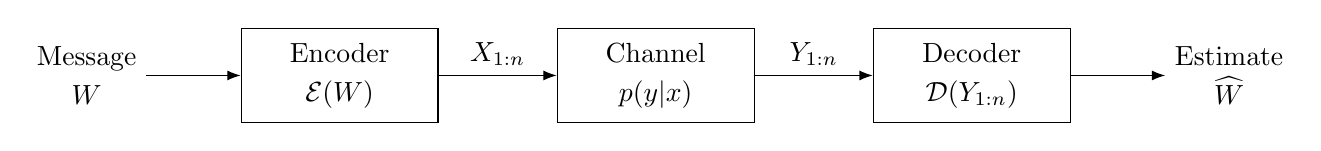
\begin{tikzpicture}[auto, node distance=1.5cm, >=Latex]
	
	% Define nodes
	\node [align=center](message) {Message \\ $W$};
	\node [draw, rectangle, right=1.2cm of message, minimum width=2.5cm, minimum height=1.2cm, align=center] (encoder) {Encoder \\ $\mathcal{E}(W)$};
	\node [draw, rectangle, right=1.5cm of encoder, minimum width=2.5cm, minimum height=1.2cm, align=center] (channel) {Channel \\ $p(y|x)$};
	\node [draw, rectangle, right=1.5cm of channel, minimum width=2.5cm, minimum height=1.2cm, align=center] (decoder) {Decoder \\ $\mathcal{D}(Y_{1:n})$};
	\node [right=1.2cm of decoder, align=center] (estimate) {Estimate \\ $\widehat{W}$};
	
	% Arrows between blocks with labels
	\draw[->] (message) -- (encoder);
	\draw[->] (encoder) -- (channel) node[midway, above] {$X_{1:n}$};
	\draw[->] (channel) -- (decoder) node[midway, above] {$Y_{1:n}$};
	\draw[->] (decoder) -- (estimate);
\end{tikzpicture}
\vspace{0.3cm}

\begin{itemize}
	\item The message $W\in\{1,\cdots,M\}$ is one of the possible $M$ numbers that we want to send. We always assume $W$ to be uniformly distributed over all possibilities.
	\item An $(M,n)$-coding scheme is an encoder $\cal{E}:\{1,\cdots,M\}\to\cal{X}^n$ that maps the message $M$ to an $n$-length string of channel inputs $X^n$;
	\item The channel specifies the probabilistic transformation from inputs to outputs:
	\begin{align*}
		p(y_{1:n}|x_{1:n})=\bbP\left(Y_1=y_1,\cdots,Y_n=y_n|X_1=x_1,\cdots,X_n=x_n\right).
	\end{align*}
We are particularly interested in the \textit{discrete memoryless channel (DMC)}, which is specified by 
\begin{itemize}
\item[(i)] an input alphabet $\cal{X}$, 
\item[(ii)] an output alphabet $\cal{Y}$, and 
\item[(iii)] a conditional probability distribution $p_{Y|X}(y|x)$ such that the outputs between channel uses are conditionally independent given the inputs:
\begin{align*}
	p(y_{1:n}|x_{1:n})=p_{Y|X}(y_1|x_1)\cdots p_{Y|X}(y_n|x_n).
\end{align*}
\end{itemize}
\item A decoder $\cal{D}:\cal{Y}^n\to\{1,\cdots,M\}$ maps an $n$-length string of channel outputs $Y_{1:n}$ to an estimate $\wh{W}$ of the transmitted message.
\end{itemize}
Now recall our two primary goals in communication:
\begin{itemize}
\item \textit{Reliability.} Assuming that the message $W$ is uniformly distributed over all possibilities, the \textit{conditional error probability} and the \textit{average error probability} are
\begin{align*}
	P_e^{(n)}(w)=\bbP(\wh{W}\neq w|W=w),\qquad P_e^{(n)}=\bbP(\wh{W}\neq W)=\frac{1}{M}\sum_{w=1}^M P_e^{(n)}(W).
\end{align*}
The maximum error probability is
\begin{align*}
	P_{\mathrm{e,max}}^{(n)}(w)=\max_{w\in\{1,\cdots,M\}}P_e^{(n)}(w)=\max_{w\in\{1,\cdots,M\}}\bbP(\wh{W}\neq w|W=w).
\end{align*}
\item \textit{Efficiency.} The \textit{rate} $R$ of an $(M,n)$ encoding scheme is
\begin{align*}
	R=\frac{\log_2 M}{n}\quad bits/transmission.
\end{align*}
Alternatively, the number of messages for a given rate $R$ and block-length $n$ is given by $M=2^{nR}$. To specify a rate $R$ code, we write $(2^{nR},n)$ instead of $(M, n)$. Particularly, are interested in the case that the error probability becomes negligible as the coding length $n$ goes infinity.
\end{itemize}


\begin{definition}[Operational Capacity]
A rate $R$ is achievable for given discrete memoryless channel $p(y|x)$, if there exists a sequence of $(\lceil 2^{nR}\rceil, n)$ coding schemes such that maximum error probability
\begin{align*}
	\lim_{n\to\infty}P_{\mathrm{e,max}}^{(n)}=0.
\end{align*}
The operational capacity $C_{\mathrm{op}}$ is the supremum over all achievable rates:
\begin{align*}
	C_{\mathrm{op}}=\sup\left\{R: R\ is\ achievable\right\}.
\end{align*}
\end{definition}

\begin{definition}[Information Capacity]
The information capacity of a discrete memoryless channel is
\begin{align*}
	C=\sup_{p_X}I(X;Y)=\sup_{p_X}\sum_{x\in\cal{X},y\in\cal{Y}}p_X(x)p_{Y|X}(y|x)\log_2\frac{p_{Y|X}(y|x)}{\sum_{x^\prime\in\cal{X}}p_{Y|X}(y|x^\prime)p_X(x^\prime)}
\end{align*}
\end{definition}
\paragraph{Remark.} Since the map $p_X,p_{Y|X}\mapsto I(X,Y)$ is concave about $p_X$, we can always find a maximizer $p_X^*$ that reaches the supremum: $C=\max_{p_X}I(X;Y)$.

\subsection{Shannon's Channel Coding Theorem: Achievability}
In the next two sections, we will establish Shannon's channel coding theorem.
\begin{theorem}[Shannon's channel coding theorem]\label{SCCT}
The operational capacity of a discrete memoryless channel is
equal to the information capacity:
\begin{align*}
	C_{\mathrm{op}}=\sup_{p_X}I(X;Y).
\end{align*}
\end{theorem}
\paragraph{Remark.} In fact, the channel coding theorem consists of two statements:
\begin{itemize}
	\item\textit{Achievability.} Every rate $R<C$ is achievable, i.e. there exists a sequence of $(2^{nR},n)$ coding schemes such that the maximum error probability $P_{\mathrm{e,max}}^{(n)}\to 0$ as $n\to\infty$:
	\begin{align*}
		R<C\quad\Rightarrow\quad R\ is\ achievable.
	\end{align*}
	\item\textit{Converse.} Any sequence of $(2^{nR},n)$ coding schemes with the maximum error probability $P_{\mathrm{e,max}}^{(n)}\to 0$ as $n\to\infty$ must satisfy $R\leq C$.
	\begin{align*}
		R\ is\ achievable\quad\Rightarrow\quad R\leq C.
	\end{align*}
\end{itemize}

\paragraph{} In this section, we are going to establish the achievability part of channel encoding theorem.

\paragraph{Construction of encoder $\cal{E}$.} A $(2^{nR},n)$ encoder $\cal{E}$ can be represented by a codebook:
\begin{align}
	\cal{E}=\begin{pmatrix}
		x_{1:n}(1) \\ x_{1:n}(2) \\ \vdots \\ x_{1:n}(2^{nR})
	\end{pmatrix} = \begin{pmatrix}
	x_1(1) & x_1(2) & \cdots & x_n(1) \\ x_1(2) & x_2(2) & \cdots & x_n(2) \\ \vdots & \vdots & \ddots & \vdots \\ x_1(2^{nR}) & x_2(2^{nR}) & \cdots & x_n(2^{nR})
\end{pmatrix}\in\cal{X}^{2^{nR}\times n}.\label{codebook}
\end{align}
To transmit a message $w$, the encoder assigns
\begin{align*}
	\cal{E}(w)=x_{1:n}(w),\quad w\in\left\{1,2,\cdots,2^{nR}\right\}.
\end{align*}
We consider the construction of random encoder. To proceed, we first choose a input distribution $p_X$. We let each entry in the codebook $\cal{E}$ to be drawn from i.i.d. $p_X$. The probability of generating any particular random codebook (\ref{codebook}) is then given by
\begin{align*}
	p(\cal{E})=\prod_w^{2^{nR}}\prod_{i=1}^n p_X(x_n(w)).
\end{align*}
With the codebook $\cal{E}$ specified, the conditional distribution of input string $X_{1:n}$ is the
\begin{align*}
	p_{X_{1:n}|\cal{E}}(x_{1:n})=\frac{1}{2^{nR}}\sum_{w=1}^{2^{nR}}\mathds{1}_{\left\{x_{1:n}=\cal{E}(w)\right\}},\quad x_{1:n}\in\cal{X}^n,
\end{align*}
and
\begin{align*}
	p_{Y_{1:n}|\cal{E}}(y_{1:n})=\frac{1}{2^{nR}}\sum_{w=1}^{2^{nR}}p_{Y_{1:n}|X_{1:n}}(y_{1:n}|\cal{E}(w)),\quad y_{1:n}\in\cal{Y}^n.
\end{align*}
To find the unconditional distribution, note that each row of the codebook has the same distribution:
\begin{align*}
	p_{X_{1:n}}(x_{1:n})&=\prod_{i=1}^n p_X(x_i);\\
	p_{Y_{1:n}}(y_{1:n})&=\sum_{x_{1:n}\in\cal{X}^n}p_{X_{1:n}}(x_{1:n})p_{Y_{1:n}|X_{1:n}}(y_{1:n}|x_{1:n})\\
	&=\sum_{x_1\in\cal{X}}\sum_{x_2\in\cal{X}}\cdots\sum_{x_n\in\cal{X}}\prod_{i=1}^np_{X}(x_i)p_{Y|X}(y_i|x_i)\\
	&=\prod_{i=1}^n\underbrace{\left(\sum_{x_i\in\cal{X}}p_X(x_i)p_{Y|X}(y_i|x_i)\right)}_{p_Y(y_i)}=\prod_{i=1}^n p_Y(y_i).
\end{align*}
Since the channel is memoryless, the \textit{information density} of $(X_{1:n},Y_{1:n})$ can be factorized:
\begin{align*}
	i(x_{1:n};y_{1:n})&=\log_2\frac{p_{X_{1:n},Y_{1:n}}(x_{1:n},y_{1:n})}{p_{X_{1:n}}(x_{1:n})p_{Y_{1:n}}(y_{1:n})}=\log_2\frac{p_{Y_{1:n}|X_{1:n}}(y_{1:n}|x_{1:n})}{p_{Y_{1:n}}(y_{1:n})}\\
	&=\sum_{k=1}^n\log_2\frac{p_{Y|X}(y_k|x_k)}{p_Y(y_k)}=\sum_{k=1}^n i(x_k;y_k).
\end{align*}
These distributions arise from the randomness in both the codebook and the message. 
\paragraph{Construction of decoder $\cal{D}$.} To finish the construction of a coding scheme, we need to find an optimal decoder. To minimize the probability of error, we use a \textit{maximum a posteriori} (MAP) decoder:
\begin{align*}
	\cal{D}^*(y_{1:n})&=\underset{w\in\{1,\cdots,2^{nR}\}}{\argmax} p_{W|Y_{1:n}}(w|y_{1:n})\\
	&=\underset{w\in\{1,\cdots,2^{nR}\}}{\argmax} p_W(w)p_{Y_{1:n}|W}(y_{1:n}|w).
\end{align*}
Since the message $W$ is uniform, the MAP decoder is equivalent to the maximum likelihood decoder:
\begin{align*}
	\cal{D}^*(y_{1:n})=\underset{w\in\{1,\cdots,2^{nR}\}}{\argmax} p_{Y_{1:n}|W}(y_{1:n}|w).
\end{align*}
Using the information density, we have
\begin{align*}
	\cal{D}^*(y_{1:n})&=\underset{w\in\{1,\cdots,2^{nR}\}}{\argmax} p_{Y_{1:n}|X_{1:n}}(y_{1:n}|x_{1:n}(w))\\
	&=\underset{w\in\{1,\cdots,2^{nR}\}}{\argmax} \frac{p_{Y_{1:n}|X_{1:n}}(y_{1:n}|x_{1:n}(w))}{p_{Y_{1:n}}(y_{1:n})}
	\\
	&=\underset{w\in\{1,\cdots,2^{nR}\}}{\argmax}i(x_{1:n}(w);y_{1:n}).
\end{align*}
To simplify the analysis, we study a sub-optimal thresholding decoder: For a given threshold $T_n$, we define the decoding rule as follows:
\begin{align*}
	\cal{D}(y_{1:n})=\begin{cases}
		\wh{w}, &if\ i(x_{1:n}(\wh{w});y_{1:n})>T_n\ and\ i(x_{1:n}(w);y_{1:n})\leq T_n\ for\ all\ w\neq\wh{w},\\
		0, &otherwise.
	\end{cases}
\end{align*}
\paragraph{Decoding error is uniform.} We now analyze the decoding error of our coding scheme. By uniformity of our construction of codebook and the message $W$,
\begin{align*}
	\bbP(\wh{W}\neq W)&=\sum_{\cal{E}}p(\cal{E})\,\bbP(\wh{W}\neq W|\cal{E})\\
	&=\sum_{\cal{E}}p(\cal{E})\sum_{w=1}^{2^{nR}}\frac{1}{2^{nR}}\bbP(\wh{W}\neq W|\cal{E},W=w)\\
	&=\frac{1}{2^{nR}}\sum_{w=1}^{2^{nR}}\sum_{\cal{E}}p(\cal{E})\bbP(\wh{W}\neq W|\cal{E},W=w)\\
	&=\frac{1}{2^{nR}}\sum_{w=1}^{2^{nR}}\sum_{\cal{E}}p(\cal{E})\bbP(\wh{W}\neq W|\cal{E},W=1)\\
	&=\sum_{\cal{E}}p(\cal{E})\bbP(\wh{W}\neq W|\cal{E},W=1)\\
	&=\bbP(\wh{W}\neq W|W=1)
\end{align*}
Therefore, it suffices to control the decoding error conditioned on the event $W=1$.

\begin{proof}[Proof of Theorem \ref{SCCT} (Achievability).]
Define events $A$ and $B$ as follows:
\begin{align*}
	A_n=\left\{i(X_{1:n}(1);Y_{1:n})>T_n\right\},\quad B_n=\bigcap_{w=2}^{2^{nR}}\left\{i(X_{1:n}(w);Y_{1:n})\leq T_n\right\}.
\end{align*}
Consider the following bound: $$P(\wh{W}\neq W|W=1)=P(A_n^c\cup B_n^c)\leq\bbP(A_n^c)+\bbP(B_n^c).$$
\textbf{Analysis of $\bbP(A_n^c)$.}  By construction, the input $X_{1:n}(1)$ and output $Y_{1:n}$ satisfies 
$$(X_k(1),Y_k)\overset{\mathrm{i.i.d.}}{\sim} p_Xp_{Y|X}.$$
Meanwhile,
\begin{align*}
	\E\left[i(X_k(1),Y_k)\right]=\E\left[\log_2\frac{p_{Y|X}(Y_k|X_k(1))}{p_Y(Y_k)}\right]=I(X;Y),\quad where\ \ (X,Y)\sim p_Xp_{Y|X}.
\end{align*}
By strong law of large numbers,
\begin{align*}
	\frac{i(X_{1:n}(1);Y_{1:n})}{n}=\frac{1}{n}\sum_{k=1}^n i(X_k(1),Y_k)\overset{a.s.}{\to} I(X;Y)\ \ as\ \ n\to\infty.
\end{align*}
Fix any $\epsilon>0$, and set $T_n=n(I(X;Y)-\epsilon)$. Hence
\begin{align*}
	\limsup_{n\to\infty}\bbP(A_n^c)&=\limsup_{n\to\infty}\bbP\left(\frac{i(X_{1:n}(1);Y_{1:n})}{n}\leq I(X;Y)-\epsilon\right)\\
	&\leq\bbP\left(\bigcap_{N=1}^\infty\bigcup_{n=N}^\infty\left\{\frac{i(X_{1:n}(1);Y_{1:n})}{n}\leq I(X;Y)-\epsilon\right\}\right)\\
	&=\bbP\left(\limsup_{n\to\infty}\frac{i(X_{1:n}(1);Y_{1:n})}{n}\leq I(X;Y)-\epsilon\right)=0.
\end{align*}
\paragraph{Analysis of $\bbP(B_n^c)$.} By construction, for all $w\neq 1$, $X_{1:n}(w)$ is independent of $X_{1:n}(1)$.  Since the output $Y_{1:n}$ is generated from $X_{1:n}(1)$ and $p_{Y|X}$, it is independent of $X_{1:n}(w)$:
$$(X_k(w),Y_k)\overset{\mathrm{i.i.d.}}{\sim} p_Xp_Y.$$
Using the Chernoff bound, we have
\begin{align*}
	\bbP\left(i(X_{1:n}(w),Y_{1:n})>T_n\right)&\leq 2^{-T_n}\E\left[2^{i(X_{1:n}(w);Y_{1:n})}\right]\\
	&=2^{-T_n}\E\left[\frac{p_{X_{1:n},Y_{1:n}}(X_{1:n}(w),Y_{1:n})}{p_{X_{1:n}}(X_{1:n}(w))p_{Y_{1:n}}(Y_{1:n})}\right]\\
	&=2^{-T_n}\sum_{x_{1:n}\in\cal{X}^n}\sum_{y_{1:n}\in\cal{Y}^n}p_{X_{1:n}}(x_{1:n})p_{Y_{1:n}}(y_{1:n})\frac{p_{X_{1:n},Y_{1:n}}(x_{1:n},y_{1:n})}{p_{X_{1:n}}(x_{1:n})p_{Y_{1:n}}(y_{1:n})}\\
	&=2^{-T_n}.
\end{align*}
We then employ a union bound:
\begin{align*}
	\bbP(B_n^c)&=\bbP\left(\bigcup_{w=2}^{2^{nR}}\left\{i(X_{1:n}(w),Y_{1:n})>T_n\right\}\right)\\
	&\leq\sum_{w=2}^{2^{nR}}\bbP\left(i(X_{1:n}(w),Y_{1:n})>T_n\right)\\
	&\leq2^{nR-T_n}\\
	&=2^{n(R-I(X;Y)+\epsilon)}.
\end{align*}
\paragraph{Choice of $\epsilon$ and $p_X$.} Since $R<C=\sup_{p_X} I(X;Y)$, we choose $\epsilon=\frac{1}{3}(C-R)$, and choose $p_X$ such that
\begin{align*}
	I(X;Y)&\geq R+2\epsilon\\
	&=C-\frac{1}{3}(C-R).
\end{align*} 
Then we have
\begin{align*}
	\lim_{n\to\infty}\bbP(\wh{W}\neq W|W=1)&\leq\lim_{n\to\infty}\bbP(A^c_n)+\lim_{n\to\infty}\bbP(B^c_n)\\
	&\leq\lim_{n\to\infty} 2^{-n\epsilon}=0.
\end{align*}
Based on our previous discussion, the result follows.

\paragraph{Strengthening the proof.} Yet we have not find a deterministic codebook with small error of probability. To finish the proof, we will strengthen this conclusion by getting rid of the average over codebooks. Note that the average probability of error over codebooks is small:
\begin{align*}
	\bbP(\wh{W}\neq W)=\sum_{\cal{E}}\bbP(\wh{W}\neq W\,|\,\cal{E})\bbP(\cal{E})<\epsilon,
\end{align*}
where $\epsilon>0$ is an arbitrarily fixed quantity. Hence, over the set of possible codebooks, there exists at least one codebook $\cal{E}^*$ with a small probability of error: $$\bbP(\wh{W}\neq W\,|\,\cal{E}=\cal{E^*})\leq\epsilon.$$ At this point, it is still possible that the codebook $\cal{E}^*$ contains some codewords with bad
conditional error probabilities. Define 
\begin{align*}
	\lambda(w)=\bbP(\wh{W}\neq W\,|\,\cal{E}=\cal{E}^*,W=w).
\end{align*}
Since $W$ is uniformly distributed over $\{1,2,\cdots,2^{nR}\}$, the number of ``bad'' codewords satisfies
\begin{align*}
	\sum_{w=1}^{2^{nR}}\mathds{1}_{\{\lambda(w)\geq 2\epsilon\}}\leq\sum_{w=1}^{nR}\frac{\lambda(w)}{2\epsilon}=\frac{1}{2\epsilon}2^{nR}\bbP(\wh{W}\neq W|\cal{E}=\cal{E^*})\leq 2^{nR\left(1-\frac{1}{n}\right)}.
\end{align*}
Therefore, if we expunge the worst half of the codewords, the maximum conditional error of the remaining codewords is $P_{e,\mathrm{max}}^{(n)}\leq 2\epsilon$, and the rate of the new codebook is
$R-\frac{1}{n}$.  Since this difference goes to zero as $n\to\infty$, we can conclude that $P_{e,\mathrm{max}}^{(n)}$ converges to $0$ as $n\to\infty$.
\end{proof}
\paragraph{Remark.} Although the theorem shows that there exist good codes with arbitrarily small error probability for long block lengths, it does not provide an approach to construct the optimal codebooks. Without some structure in the code, the simple decoding scheme of table lookup requires an exponentially large table. 

\subsection{Shannon's Channel Coding Theorem: Weak Converse}
In this section, we prove the converse part of Shannon's channel coding theorem.
\begin{lemma}\label{scctconverselemma}
Let $C=\sup_{p_X}(X;Y)$ be the information capacity of a discrete memoryless channel $p_{Y|X}$. For any input distribution $p_{X_{1:n}}(x_{1:n})$, it holds
\begin{align*}
	I(X_{1:n};Y_{1:n})\leq nC.
\end{align*}
\end{lemma}
\begin{proof}
We decompose the mutual information $I(X_{1:n};Y_{1:n})$ by chain rule:
\begin{align*}
	I(X_{1:n};Y_{1:n})&=H(Y_{1:n})-H(Y_{1:n}|X_1,\cdots,X_n)\\
	&=\sum_{i=1}^n H(Y_{i}|Y_{i-1},\cdots,Y_1)-\sum_{i=1}^n H(Y_{i}|Y_{i-1},\cdots,Y_1,X_1,\cdots,X_n)\\
	&=\sum_{i=1}^n H(Y_{i}|Y_{i-1},\cdots,Y_1)-\sum_{i=1}^n H(Y_i|X_i)\\
	&\leq\sum_{i=1}^n H(Y_{i})-\sum_{i=1}^n H(Y_i|X_i)=\sum_{i=1}^n I(X_i;Y_i)\leq nC.
\end{align*}
Hence we conclude the proof.
\end{proof}
\begin{proof}[Proof of Theorem \ref{SCCT} (Converse).]
By Fano's inequality [Theorem \ref{fanoineq}], 
\begin{align*}
	P_e^{(n)}=\bbP(\wh{W}\neq W)\geq\frac{H(W|\wh{W})-1}{\log_2 2^{nR}}=\frac{H(W|\wh{W})-1}{nR}.
\end{align*}
Since $W$ is uniform over all possibilities,
\begin{align*}
	nR=H(W)&=H(W|\wh{W})+I(W;\wh{W})=nRP_e^{(n)}+1+I(W;\wh{W})\\
	&\leq nRP_e^{(n)}+1+I(X_{1:n};Y_{1:n})\tag{By data processing inequality}\\
	&\leq nRP_e^{(n)}+1+nC.
\end{align*}
Therefore, we have
\begin{align*}
	P_e^{(n)}\geq\frac{n(R-C)-1}{nR}\geq 1-\frac{C}{R},\quad\forall n\in\bbN.
\end{align*}
If $R>C$, the error probability $P_e^{(n)}$ does not converge to $0$, and $R$ is not achievable.
\end{proof}

\paragraph{Further discussion about random coding: Privacy.} We will provide more analysis about the privacy of this random coding scheme. Suppose that an eavesdropper observes the channel output $Y_{1:n}$ but does not know the
codebook $\cal{E}$. We are worried that the eavesdropper might figure out the codebook. 

Since the codebook $\cal{E}$ is randomly chosen, the difficulty of recovering the codebook $\cal{E}$ from the outputs $Y_{1:n}$ depends on the their mutual information. We will prove the following bound:
\begin{align*}
	I(\mathcal{E};Y_{1:n})\leq n(C-R)+H_b(P_e^{(n)})+P_e^{(n)}nR.
\end{align*}
Using the chain rule, we have the decomposition
\begin{align*}
	I(\mathcal{E};Y_{1:n})=I(Y_{1:n};\cal{E},W)-I(Y_{1:n};W\,|\,\cal{E}).
\end{align*}
\begin{itemize}
\item We first bound $I(Y_{1:n};\cal{E},W)$. Since $X_{1:n}$ is a function of $W$ and $\cal{E}$, and $Y_{1:n}$ is conditionally independent of $\cal{E},W$ given $X_{1:n}$,
	\begin{align*}
		I(Y_{1:n};\cal{E},W)=I(Y^n;\cal{E},W,X_{1:n})=I(Y_{1:n};X_{1:n})\leq nC.
	\end{align*}
	where the last inequality follows from Lemma \ref{scctconverselemma}.
	
\item Now we bound $I(Y_{1:n};W\,|\,\cal{E})$. Since the message $W$ and the codebook $\cal{E}$ are independent, we have
	\begin{align*}
		I(W;Y_{1:n}\,|\,\cal{E})=I(W;Y_{1:n},\cal{E})-I(W;\cal{E})=I(W;Y_{1:n},\cal{E}).
	\end{align*}
	Since $W$ is conditionally independent of $\wh{W}$ given $Y^n$ and $\cal{E}$, we have
	\begin{align*}
		I(W;Y_{1:n}\,|\,\cal{E})=I(W;Y_{1:n},\cal{E})&\geq I(W;\wh{W},\cal{E})\tag{data processing inequality}\\
		&=H(W)-H(W|\wh{W},\cal{E})\tag{chain rule}\\
		&\geq H(W)-H(W|\wh{W}).\tag{Conditioning does not increase entropy}
	\end{align*}
	By Fano's inequality,
	\begin{align*}
		H(W\,|\,\wh{W})\leq H_b(P_e^{(n)})+P_e^{(n)}\log\vert\cal{W}\vert\leq nRP_e^{(n)}+H_b(P_e^{(n)}).
	\end{align*}
	Note that $W\sim\mathrm{Unif}(1,2,\cdots,2^{nR})$, we have
	\begin{align*}
		I(W;Y_{1:n}\,|\,\cal{E})\geq H(W)-H(W|\wh{W})=(1-P_e^{(n)})nR-H_b(P_e^{(n)}).
	\end{align*}
\end{itemize}
According to the two bounds, we have
\begin{align*}
	I(\mathcal{E};Y_{1:n})&=I(Y_{1:n};\cal{E},W)-I(Y_{1:n};W\,|\,\cal{E})\leq nC-(1-P_e^{(n)})nR+H_b(P_e^{(n)}).
\end{align*}
This proves the result. As long as the error probability $P_e^{(n)}$ is sufficiently small, increasing the rate $R$ leads to better privacy. An interpretation is that a coding scheme with higher rate $R$ produces less redundancy while transmitting a message. In this case, there is less information about the codebook $\cal{E}$ in the output $Y_{1:n}$.
\newpage
\subsection{Feedback Capacity}
We turn to another setting of channel coding, where we allow our encoder to use previous outputs. That is, at the $n$-th step, our encoder assigns a channel input $X_n$ according to not only the message $W$ to be transmitted, but also the previous outputs $Y_{1:(n-1)}$. This setting is called the channel coding with \textit{feedback}.

\vspace{0.4cm}

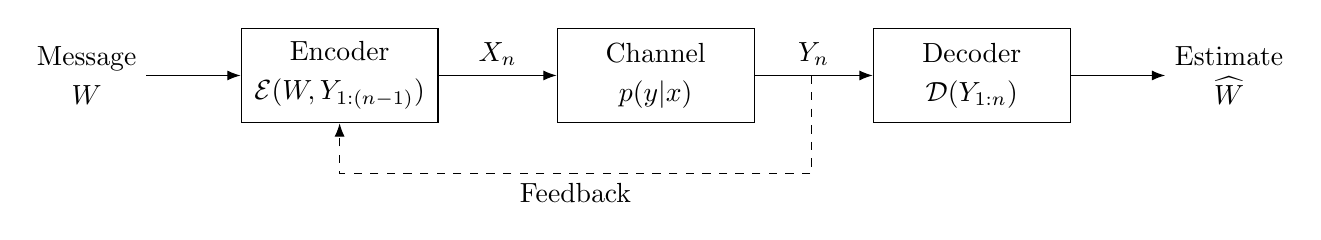
\begin{tikzpicture}[auto, node distance=1.5cm, >=Latex]
	
	% Define nodes
	\node [align=center](message) {Message \\ $W$};
	\node [draw, rectangle, right=1.2cm of message, minimum width=2.5cm, minimum height=1.2cm, align=center] (encoder) {Encoder \\ $\mathcal{E}(W, Y_{1:(n-1)})$};
	\node [draw, rectangle, right=1.5cm of encoder, minimum width=2.5cm, minimum height=1.2cm, align=center] (channel) {Channel \\ $p(y|x)$};
	\node [draw, rectangle, right=1.5cm of channel, minimum width=2.5cm, minimum height=1.2cm, align=center] (decoder) {Decoder \\ $\mathcal{D}(Y_{1:n})$};
	\node [right=1.2cm of decoder, align=center] (estimate) {Estimate \\ $\widehat{W}$};
	
	% Arrows between blocks with labels
	\draw[->] (message) -- (encoder);
	\draw[->] (encoder) -- (channel) node[midway, above] {$X_n$};
	\draw[->] (channel) -- (decoder) node[midway, above] {$Y_n$};
	\draw[->] (decoder) -- (estimate);
	
	% Feedback arrow starting from Y_n label
	\draw[->, dashed] (channel.east) ++(0.72,0) |- ++(0,-1.25) -| (encoder.south) node[pos=0.25, below] {Feedback};
	
\end{tikzpicture}

\begin{theorem}
Feedback \textit{cannot} increase capacity. For a discrete memoryless channel, the capacity with feedback, $C_\mathrm{FB}$, is the same as the capacity without feedback:
$$C_\mathrm{FB} = C.$$
\end{theorem}
\begin{proof}
Like the proof of the weak converse, since $W$ is uniform over all possibilities,
\begin{align*}
	nR=H(W)&=H(W|\wh{W})+I(W;\wh{W})\\
	&=nRP_e^{(n)}+1+I(W;\wh{W})\tag{By Fano's inequality}\\
	&\leq nRP_e^{(n)}+1+I(W;Y_{1:n})\tag{By data processing inequality}.
\end{align*}
Then it remains to bound the mutual information $I(W;Y_{1:n})$. Since $X_i$ is a function of $W$ and $(Y_{i-1},\cdots,Y_i)$, and $Y_i$ is conditionally independent of $W$ and $(Y_{i-1},\cdots,Y_i)$ given $X_i$, we have
\begin{align*}
	H(Y_{i}|Y_{i-1},\cdots,Y_1,W)=H(Y_{i}|Y_{i-1},\cdots,Y_1,W,X_i)=H(Y_{i}|X_i)
\end{align*}
Then
\begin{align*}
	I(W;Y_{1:n})&=H(Y_{1:n})-H(Y_{1:n}|W)\\
	&=\sum_{i=1}^n H(Y_{i}|Y_{i-1},\cdots,Y_1)-\sum_{i=1}^n H(Y_{i}|Y_{i-1},\cdots,Y_1,W)\\
	&=\sum_{i=1}^n H(Y_{i}|Y_{i-1},\cdots,Y_1)-\sum_{i=1}^n H(Y_i|X_i)\\
	&\leq\sum_{i=1}^n H(Y_{i})-\sum_{i=1}^n H(Y_i|X_i)\\
	&=\sum_{i=1}^n I(X_i;Y_i)\leq nC.
\end{align*}
Therefore,
\begin{align*}
	P_e^{(n)}\geq\frac{n(R-C)-1}{nR}\geq 1-\frac{C}{R},\quad\forall n\in\bbN.
\end{align*}
If $R>C$, the error probability $P_e^{(n)}$ does not converge to $0$, and $R$ is not achievable. Hence $R\leq C$.
\end{proof}
\paragraph{Remark.} This surprising fact stems from the memorylessness of the channel. Of course, feedback can help simplify our encoding and decoding schemes in terms of complexity.

\subsection{Hamming Code}
\paragraph{Motivation.} The object of coding is to introduce \textit{redundancy} so that even if some of the information is lost or corrupted, it is still possible to recover the message at the receiver. 

A simplest coding scheme is to repeat information.  For example, consider sending a bit $W\in\{0,1\}$ with a binary symmetric channel. One repeat the bit over $n$ channel uses, i.e. send $\underbrace{11\cdots 1}_{n}$ for $1$ and $\underbrace{00\cdots 0}_{n}$ for $0$. This code can correct up to $\frac{n-1}{2}$ flips, and the error probability converges to $0$ as $n\to\infty$.
However, the rate $R=1/n$ of this code also goes to $0$, which is not very useful.

\paragraph{Parity check code.} Instead of simply repeating the bits, we can introduce each extra bit to check whether there is an error in some subset of the information bits. This is called an \textit{error-detecting code.}

A \textit{single parity check} code is a $(2^{n-1}, n)$ coding scheme for a binary symmetric channel which sends $n-1$ information bits, and the $n$-th bit encodes the \textit{parity} of the entire block, i.e. whether the number of 1’s in the information bits is even or odd. Then if there is an odd number of errors during transmission, the receiver will notice that the parity has changed and detect the error. This code does not detect an even number of errors and does not give any information about how to correct the errors that occur.

\paragraph{Hamming Code.} To illustrate the idea of Hamming codes, we begin with an $m\times(2^m-1)$ binary matrix formed by arranging the $2^m-1$ nonzero binary column vectors of length $m$ in ascending order. The matrix $H$ is called a \textit{parity check matrix}. For example, when $m=3$, the parity check matrix $H\in\{0,1\}^{3\times 7}$ is given by
\begin{align*}
	H=\begin{bmatrix}
		0 & 0 & 0 & 1 & 1 & 1 & 1\\
		0 & 1 & 1 & 0 & 0 & 1 & 1\\
		1 & 0 & 1 & 0 & 1 & 0 & 1
	\end{bmatrix}.
\end{align*}
From now on, all operations will be done modulo 2. Under this setting, the set $\{0,1\}$ becomes a field:
\begin{align*}
	0\pm 0=0,\quad 0\pm 1=1,\quad 1\pm 1=0,\qquad 0\cdot 0=0,\quad 0\cdot 1=0,\quad 1\cdot 1=1,\qquad\frac{0}{1}=0,\quad\frac{1}{1}=1.
\end{align*}  
The \textit{Hamming codewords} correspond to the \textit{null space of the parity check matrix}. In other words, each Hamming codeword $c$ is a solution of the linear system
\begin{align*}
	Hc=0,
\end{align*}
where $c\in\{0,1\}^{2^m-1}$ is a binary vector. For the case $m=3$, there are $16$ Hamming codewords:
\begin{align}
	\begin{matrix}
		0000000 & 0100101 & 1000011 & 1100110\\
		0001111 & 0101010 & 1001100 & 1101001\\
		0010110 & 0110011 & 1010101 & 1110000\\
		0011001 & 0111100 & 1011010 & 1111111
	\end{matrix}\label{hammingcode74}
\end{align}
We call this a \textit{$(7,4)$ Hamming code}, and the rate is
\begin{align*}
	R=\frac{\log_2 16}{7}=\frac{4}{7}.
\end{align*}

Furthermore, since the null space $\ker(H)$ is a subspace of the vector space $\{0,1\}^{2^m-1}$, the sum of any two codewords is also a codeword.

\paragraph{Rate of the Hamming code.} According the rank-nullity theorem, for a parity matrix $H\in\{0,1\}^{m\times(2^m-1)}$,
\begin{align*}
	\mathrm{rank}(H)+\dim\ker(H)=2^m-1.
\end{align*}
Since we can always pick the $m$ distinct one-hot vectors from the columns of $H$, we have $\mathrm{rank}(H)=m$, and $\dim\ker(H)=2^m-m-1$. Therefore, the null space of $H$ has dimension $k=2^m-m-1$, and over the binary field there are $2^k$ Hamming codewords. This is called a \textit{$(N,k)$ Hamming code}, which carries $k=2^m-m-1$ information bits via $N=2^m-1$ channel uses. The rate of this code is
\begin{align*}
	R=\frac{k}{N}=1-\frac{m+1}{2^m-1}.
\end{align*}
As we can see, the rate $R$ of the Hamming code converges to $1$ as $m\to\infty$.

\paragraph{Minimum weight and minimum distance.}
Since the columns of $H$ are distinct, the sum of any two columns of $H$ must not be the all-0 vector. Hence the minimum number of 1's in any nonzero codeword is 3. This is called the \textit{minimum weight} of the Hamming code.

If $c_1\neq c_2$ are two distinct Hamming codewords, we have $H(c_1-c_2)=0$, and $c_1-c_2$ has minimum weight $3$. Hence $c_1$ and $c_2$ differ at no less than $3$ bits. This is called the \textit{minimum distance} of the Hamming code.

\paragraph{Covering property of the Hamming codewords.} We can show that the Hamming words are widely dispersed in the space of bit words. Let $c\in\{0,1\}^{2^m-1}$ be a Hamming codeword, and write by $[c]$ the ball centered at $c$ of radius $1$ in $\{0,1\}^{2^m-1}$, i.e. $[c]$ is set of all bit words of length $2^m-1$ whose distance to $c$ is not greater than $1$. For example, when $m=3$ and $c=0100101$,
\begin{align*}
	[0100101]=\left\{0100101,1100101,0000101,0110101,0101101,0100001,0100111,0100100\right\}
\end{align*}

Generally, the ball $[c]$ contains $2^m$ words, which are $c$ it self and the $2^m-1$ words obtained by flipping exactly one bit of $c$. Since the minimum distance of the Hamming code is $3$, we have $[c]\cap[\wt c]=\emptyset$ for any codewords $c\neq \wt c$. As a result, there are $2^k\cdot 2^m=2^{2^m-1}$ distinct bit words in the union of the unit balls centered the Hamming codewords $c_1,c_2,\cdots, c_{2^k}$. Since there are in total $2^{2^m-1}$ bit words of length $2^m-1$,
\begin{align*}
	\{0,1\}^{2^m-1}=[c_1]\cup[c_2]\cup\cdots\cup\left[c_{2^k}\right]
\end{align*}
Thus we obtain a cover of the space of all bit words generated by the Hamming codewords. In this sense, every bit word of length $2^m-1$ either is a codeword or differs from a unique codeword in exactly $1$ bit.

\paragraph{Hamming code corrects up to $1$ flip.} If a codeword $c$ is corrupted in only one bit, it will differ from any other codeword in at least two bits. Hence $c$ is the unique closest codeword.

In fact, we can identify the closest codeword without a brutal search of all codewords. We assume that $e_i$ is the one-hot vector whose $i^\text{th}$ bit is $1$. If the $i^\text{th}$ bit of the codeword $c$ is flipped, the received vector is then given by $r=c+e_i$, which satisfies
\begin{align*}
	Hr=H(c+e_i)=Hc+He_i=He_i.
\end{align*}
This is simply the $i^\text{th}$ column of the parity check matrix $H$.

Thus, assuming that only one bit was flipped, the vector $Hr$ is the binary representation of index of the flipped bit. By flipping this bit in the received vector $r$, we recover the original codeword $c$.

\paragraph{Application: the hat game.} We see an application of the Hamming code in game theory. In a \textit{hat game} of $N$ players, each player is independently assigned a hat. Each hat is colored $0$ or $1$ with probability $1/2$. Here are the rules of the game:
\begin{itemize}
\item Players act a team – everyone wins or everyone loses.
\item A player can observe the hats of all other players, but cannot observe the color of her own hat.
\item Once hats have been distributed, there no communication between team members.
\item When asked the color of their hats, all players must answer simultaneously.
\item Each person is allowed to pass rather than guess a color.
\item Team wins if at least one player guesses correctly and none guess incorrectly. Otherwise, the team loses.
\end{itemize}
We focus on finding an optimal strategy that maximizes the winning rate. Before we proceed, let us take a look at the best result the players can make. We let $x_i$ be the color of the $i^\text{th}$ player's hat.
\begin{itemize}
\item In this game, each player's decision making process is independent of the color of their own hat. 

\item If the $j^{\mathrm{th}}$ player gives a correct guess in the case $(x_1,\cdots,x_{j-1},0,x_{j+1},\cdots,x_N)$, she must give a wrong guess in the case $(x_1,\cdots,x_{j-1},1,x_{j+1},\cdots,x_N)$, and vice versa. Therefore, no matter what strategy the players take, there must be an equal number of correct and wrong guesses among all possible outcomes.

\item However, this fact does not mean that our overall strategy has to lose as much as it wins! According to the rule, we require each win to have at least one correct guess and no wrong guess. To increase our overall winning rate, we would like that there are less correct guesses in each win and more wrong guesses in each loss. In the optimal case, we would have exactly one correct guess in every win.

\item Among all $2^N$ outcomes, we assume that there are $G$ wins. According to the constraint we discussed previously, to maximize $G$, we assume that each win has only a single correct guess. Since each loss has up to $N$ wrong guesses, we have
\begin{align*}
	G\leq N(2^N-G).
\end{align*}
\end{itemize}
This gives an upper bound of the winning rate, and we cannot do any better:
\begin{align*}
	\bbP(win)=\frac{G}{2^N}\leq\frac{N}{N+1}.
\end{align*}

\paragraph{The optimal strategy.} In the hat game, when the number of the players is of the form $N=2^m-1$, we consider the following strategy: Player $j$ forms the bit word $(x_1,\cdots,x_{j-1},*,x_{j+1},\cdots,x_N)$, where $x_i$ is the color of the $i^\text{th}$ hat.
\begin{itemize}
\item If $(x_1,\cdots,x_{j-1},0,x_{j+1},\cdots,x_N)$ forms a Hamming codeword, the player $j$ guesses $1$;
\item If $(x_1,\cdots,x_{j-1},1,x_{j+1},\cdots,x_N)$ forms a Hamming codeword, the player $j$ guesses $0$;
\item Otherwise, the player $j$ passes.
\end{itemize}
Using this strategy, there are only two possible outcomes:
\begin{itemize}
\item If $(x_1,\cdots,x_n)$ is not a Hamming codeword, then it differs from a unique Hamming codeword in exactly one bit, denoted by $x_j$. In this case, all players except $j$ pass and the player $j$ gives a correct guess.
\item If $(x_1,\cdots,x_n)$ is a Hamming codeword, then each player gives a wrong guess.
\end{itemize}
Then the winning rate is one minus the proportion of Hamming codewords to all bit words:
\begin{align*}
	\bbP(win)=1-\frac{2^k}{2^N}=\frac{2^{2^m-m-1}}{2^{2^m-1}}=1-2^{-m}=\frac{N}{N+1}.
\end{align*}
Hence this strategy reaches the optimal winning rate. Furthermore, the winning rate converges to $1$ as $m\to\infty$.



\newpage
\section{Differential Entropy and Gaussian Channels}
\subsection{Differential Entropy of Continuous Random Variables}
\paragraph{Motivation: Entropy of continuous random variables.} We let $X$ be a continuous real-valued random variable supported on $[a,b]$. Assume that the density function $f$ of $X$ is a continuous function. Then
\begin{align*}
	\bbP(X\leq x)=\int_a^x f(t)\,dt,\quad a\leq x\leq b.
\end{align*}
We divide the range of $X$ into bins of width $\delta>0$:
\begin{align*}
	a=t_0<t_1<t_2<\cdots<t_{n-1}<b<t_n,\quad t_i-t_{i-1}=\delta.
\end{align*}
By mean-value theorem, there exists $x_i\in[t_{i-1},t_i]$ such that
\begin{align*}
	f(x_i)\delta=\int_{t_{i-1}}^{t_i}f(x)\,dx.
\end{align*}
We then quantize $X$ by defining
\begin{align*}
	X^\delta=x_i,\quad if\ \ t_{i-1}\leq X < t_i.
\end{align*}
Then $X^\delta$ is a discrete random variable, and its probability mass function is given by
\begin{align*}
	\bbP(X^\delta=x_i)=\int_{t_{i-1}}^{t_i}f(x)\,dx=f(x_i)\delta.
\end{align*}
The entropy of $X^\delta$ is
\begin{align*}
	H(X^\delta)=\sum_{i=1}^n f(x_i)\delta\log\frac{1}{f(x_i)\delta}&=\sum_{i=1}^n f(x_i)\delta\frac{1}{f(x_i)}+\sum_{i=1}^n f(x_i)\delta\log\frac{1}{\delta}\\
	&=\sum_{i=1}^n(t_i-t_{i-1}) f(x_i)\log\frac{1}{f(x_i)}+\log\frac{1}{\delta}\sum_{i=1}^n \int_{t_{i-1}}^{t_i}f(x)\,dx\\
	&=\sum_{i=1}^n(t_i-t_{i-1}) f(x_i)\log\frac{1}{f(x_i)}+\log\frac{1}{\delta}.
\end{align*}
This entropy blows up as $\delta\to\infty$. Therefore, the entropy of a continuous random variable is infinite. However, since $f:[a,b]\to\bbR_+$ is Riemann integrable, we have
\begin{align*}
	\lim_{\delta\downarrow 0}\left(H(X^\delta)-\log\frac{1}{\delta}\right)&=\int_a^b f(x)\log\frac{1}{f(x)}\,dx\\
	&=\E\left[\log\frac{1}{f(X)}\right].
\end{align*}
We can extend this definition to multidimensional spaces.

\begin{definition}[Differential entropy]\label{diffentropy}
Let $X\sim f$ be a continuous random variable, and the range of $X$ is $\cal{X}\subset\bbR^p$. If the function $x\mapsto f(x)\log f(x)$ is integrable, define the \textit{differential entropy of $X$} to be
\begin{align*}
	h(X)=\int_{\cal{X}} f(x)\log\frac{1}{f(x)}\,dx=-\E\left[\log f(X)\right].
\end{align*}
\end{definition}

\begin{example} Here are some examples of differential entropy.
\begin{itemize}
\item[(i)] Let $X$ be a uniform random variable on $[0,a]$. Then $h(X)=\int_0^a\frac{1}{a}\log a\,dx=\log a$. When $0<a<1$, we have $h(X)<0$. It is seen that the differential entropy can be negative!
\item[(ii)] Let $X\sim N(0,\sigma^2)$ be a Gaussian random variable. Then
\begin{align*}
	h(X)=\int_{-\infty}^\infty\frac{1}{\sqrt{2\pi}\sigma}\e^{-\frac{x^2}{2\sigma^2}}\left(\log\left(\sqrt{2\pi}\sigma\right)+\frac{x^2}{2\sigma^2}\right)\,dx=\frac{1}{2}+\frac{1}{2}\log\left(2\pi\sigma^2\right).
\end{align*}
\item[(iii)] Let $X\sim N(0,\Sigma)$ be a $p$-dimensional Gaussian random vector, where the covariance matrix $\Sigma\in\bbR^{p\times p}$ is nonsingular. Then
\begin{align*}
	h(X)&=\int_{\bbR^p}\frac{1}{(2\pi)^{p/2}\det(\Sigma)^{1/2}}\e^{-\frac{1}{2}x^\top\Sigma^{-1} x}\left(\log\left((2\pi)^{p/2}\det(\Sigma)^{1/2}\right)+\frac{1}{2}x^\top\Sigma^{-1}x\right)\,dx\\
	&=\frac{p}{2}\log(2\pi)+\frac{1}{2}\log\det(\Sigma)+\underbrace{\frac{1}{2}\E\left[X^\top\Sigma^{-1}X\right]}_{=\frac{1}{2}\tr(\Sigma^{-1}\E\left[XX^\top\right])}\\
	&=\frac{p}{2}\log(2\pi\e)+\frac{1}{2}\log\det(\Sigma).
\end{align*}
\end{itemize}
\end{example}
The definition of conditional differential entropy, mutual information and relative entropy then follows from the differential entropy.
\begin{definition}
Let $X,Y,Z\sim f$ be three continuous random variables. For brevity, we also write $f(x)$ and $f(y)$ for the marginal density function of $X$ and $Y$, respectively.
\begin{itemize}
\item[(i)] The \textit{joint differential entropy} between $X$ and $Y$ is the differential entropy of the random vector $(X,Y)$;
\item[(ii)] The \textit{conditional differential entropy} of $Y$ given $X$ is
\begin{align*}
	h(Y|X)=-\int_{\cal{X}\times\cal{Y}}f(x,y)\log f(y|x)\,dx\,dy.
\end{align*}
\item[(iii)] The \textit{mutual information} between $X$ and $Y$ is
\begin{align*}
	I(X;Y)=\int_{\cal{X}\times\cal{Y}}f(x,y)\log\frac{f(x,y)}{f(x)f(y)}\,dx\,dy.
\end{align*}
\item[(iv)] The \textit{conditional mutual information} between $X$ and $Y$ given $Z$ is
\begin{align*}
	I(X;Y|Z)=\int_{\cal{X}\times\cal{Y}\times{Z}}f(x,y,z)\log\frac{f(x,y|z)}{f(x|z)f(y|z)}\,dx\,dy\,dz.
\end{align*}
\item[(v)] Given two density functions $f$ and $g$ defined in the same space $\cal{X}\subset\bbR^p$ such that $g\ll f$, i.e. $g(x)=0$ for all $x\in U$ with $f(x)=0$. Then the \textit{Kullback-Leibler divergence} of $g$ from $f$  is
\begin{align*}
	D(f\,\Vert\,g):=\int_\cal{X}f(x)\log\frac{f(x)}{g(x)}\,dx=\E_{X\sim f}\left[\log\frac{f(X)}{g(X)}\right].
\end{align*}
\end{itemize}
\end{definition}
\paragraph{Remark.} Many identities and inequalities in the discrete case also applies to the continuous case:
\begin{itemize}
\item $h(X,Y)=h(X)+h(Y|X)$.
\item $I(X;Y)=h(Y)-h(Y|X)=h(X)-h(X|Y)$.
\item $I(X;Y)=D(f_{XY}\,\Vert\, f_Xf_Y)$.
\item $I(X;Y|Z)=h(X|Z)-h(X|Y,Z)=h(Y|Z)-h(Y|X,Z)$.
\item $I(X;Y,Z)=I(X;Z)+I(X;Y|Z)$.
\end{itemize}

\begin{example}
We aim to compute the mutual information between two jointly Gaussian variables.
\begin{itemize}
\item[(a)] Let $X$ and $Y$ be two jointly Gaussian random vectors:
$$\begin{pmatrix}
	X \\ Y
\end{pmatrix}\sim \cal{N}\left(\begin{pmatrix}
	0 \\ 0
\end{pmatrix},\begin{pmatrix}
	\Sigma_{11} & \Sigma_{12} \\ \Sigma_{21} & \Sigma_{22}
\end{pmatrix}\right),$$
where $\Sigma_{11}\in\bbR^{p\times p}$ and $\Sigma_{22}\in\bbR^{q\times q}$ are both nonsingular, and the covariance matrix $\Sigma=\begin{pmatrix}
	\Sigma_{11} & \Sigma_{12} \\ \Sigma_{21} & \Sigma_{22}
\end{pmatrix}$ is also nonsingular. Then
\begin{align*}
	h(Y|X)&=\int_{\bbR^p}f(x)\int_{\bbR^q}f(y|x)\log\frac{1}{f(y|x)}\,dy\,dx\\
	&=\int_{\bbR^p}f(x)\left(\frac{p}{2}\log(2\pi e)+\frac{1}{2}\log\det(\Sigma_{22.1})\right)dx\\
	&=\frac{q}{2}\log(2\pi\e)+\frac{1}{2}\log\det(\Sigma_{22.1})
\end{align*}
where the conditional covariance matrix is $\Sigma_{22.1}=\Sigma_{22}-\Sigma_{21}\Sigma_{11}^{-1}\Sigma_{12}$. By Schur complement, 
\begin{align*}
	\det(\Sigma)=\det(\Sigma_{11})\det(\Sigma_{22.1})\quad\Rightarrow\quad \log\det(\Sigma)=\log\det(\Sigma_{11})+\log\det(\Sigma_{22.1}).
\end{align*}
Therefore,
\begin{align*}
	I(X;Y)&=h(Y)-h(Y|X)\\
	&=\frac{q}{2}\log(2\pi\e)+\frac{1}{2}\log\det(\Sigma_{11})-\frac{q}{2}\log(2\pi\e)-\frac{1}{2}\log\det(\Sigma_{22.1})\\
	&=\frac{1}{2}\log\frac{\det(\Sigma_{11})\det(\Sigma_{22})}{\det(\Sigma)}.
\end{align*}
To summarize,
\begin{align*}
	h(Y|X)=\frac{q}{2}\log(2\pi\e)+\frac{1}{2}\log\frac{\det(\Sigma)}{\det(\Sigma_{11})},\quad h(X|Y)=\frac{p}{2}\log(2\pi\e)+\frac{1}{2}\log\frac{\det(\Sigma)}{\det(\Sigma_{22})},
\end{align*}
and
\begin{align*}
	I(X;Y)=\frac{1}{2}\log\frac{\det(\Sigma_{11})\det(\Sigma_{22})}{\det(\Sigma)}.
\end{align*}
In particular, if $X$ and $Y$ are independent, the covariance matrix is $\Sigma=\begin{pmatrix}
	\Sigma_{11} & 0 \\ 0 & \Sigma_{22}
\end{pmatrix}$, and $I(X;Y)=0$.
\item[(b)] We consider the bivariate Gaussian distribution:
$$\begin{pmatrix}
	X \\ Y
\end{pmatrix}\sim \cal{N}\left(\begin{pmatrix}
	0 \\ 0
\end{pmatrix},\begin{pmatrix}
	\sigma_1^2 & \rho\sigma_1\sigma_2 \\ \rho\sigma_2\sigma_1 & \sigma_2^2
\end{pmatrix}\right),$$
where $\rho\in(-1,1)$ is the correlation coefficient between $X$ and $Y$. Then
\begin{align*}
	I(X;Y)=\frac{1}{2}\log\frac{1}{1-\rho^2}.
\end{align*}
In particular, if $\rho=0$, the mutual information between $X$ and $Y$ is $0$; and if $\rho=\pm 1$, the mutual information between $X$ and $Y$ is infinity.
\item[(c)] Let $X\sim\cal{N}(\mu_1,\Sigma_1)$ and $Y\sim\cal{N}(\mu_2,\Sigma_2)$, where $\Sigma_1,\Sigma_2\in\bbR^{p\times p}$. Then
\begin{align*}
	D(X\Vert Y)&=\E\left[\log\frac{f_X(X)}{f_Y(X)}\right]\\
	&=\frac{1}{2}\log\frac{\det(\Sigma_2)}{\det(\Sigma_1)}-\frac{1}{2}\E\left[(X-\mu_1)^\top\Sigma_1^{-1}(X-\mu_1)\right]+\frac{1}{2}\E\left[(X-\mu_2)^\top\Sigma_2^{-1}(X-\mu_2)\right]\\
	&=\frac{1}{2}\log\frac{\det(\Sigma_2)}{\det(\Sigma_1)}-\frac{p}{2}+\frac{1}{2}\tr\left(\Sigma_2^{-1}\E\left[(X-\mu_2)(X-\mu_2)^\top\right]\right)\\
	&=\frac{1}{2}\log\frac{\det(\Sigma_2)}{\det(\Sigma_1)}-\frac{p}{2}+\frac{1}{2}\left((\mu_1-\mu_2)^\top\Sigma_2(\mu_1-\mu_2)+\tr(\Sigma_2^{-1}\Sigma_1)\right).
\end{align*}
\end{itemize}
\end{example}
\begin{theorem}[Linear transformation]
Let $A\in\bbR^{p\times p}$ be a nonsingular matrix, and $b\in\bbR^p$. Let $X$ be a continuous $p$-dimensional random vector. Then
\begin{align*}
	h(AX+b)=h(X)+\log\left\vert\det(A)\right\vert.
\end{align*}
\end{theorem}
\begin{proof}
Let $Y=AX$. If $X$ has density function $f$, the density of $Y$ is given by
\begin{align*}
	g(y)=\frac{f(A^{-1}y)}{\left\vert\det(A)\right\vert},\quad y\in\bbR^p.
\end{align*}
Then the differential entropy of $Y$ is
\begin{align*}
	h(Y)&=-\int_{\bbR^p}g(y)\log g(y)\,dy\\
	&=-\int_{\bbR^p}\frac{f(A^{-1}y)}{\left\vert\det(A)\right\vert}\log\frac{f(A^{-1}y)}{\left\vert\det(A)\right\vert}\,dy\\
	&=-\int_{\bbR^p}\frac{f(x)}{\left\vert\det(A)\right\vert}\log\frac{f(x)}{\left\vert\det(A)\right\vert}\left\vert\det(A)\right\vert dx\tag{change the variable $x=A^{-1}y$}\\
	&=-\int_{\bbR^p}f(x)\log f(x)\,dx+\int_{\bbR^n}f(x)\log\left\vert\det(A)\right\vert\,dx\\
	&=h(X)+\log\left\vert\det(A)\right\vert.
\end{align*}
By change the variable $Z=Y+b=Ax+b$, we know that $h(Z)=h(Y)$. This is the desired result.
\end{proof}
\paragraph{Remark.} This transformation formula also holds for conditional differential entropy. Analogous to this formula, we have the transformation invariance for mutual information and KL-divergence:
\begin{align*}
	h(Ax+b|Y)&=h(X|Y)+\log\left\vert\det(A)\right\vert,\\
	I(AX+b;Y)&=I(X;Y),\\
    D(f_{Ax+b}\Vert f_{AY+b})&=D(f_X\Vert f_Y).
\end{align*}

We have the following estimate for the differential entropy of a random vector.
\begin{theorem}[Upper bound of the differential entropy]\label{gaussmaxdiffent}
If $X$ is a $p$-dimensional random vector with mean $\mu\in\bbR^p$ and covariance matrix $\Sigma\in\bbR^{p\times p}$,
\begin{align*}
	h(X)\leq \frac{p}{2}\log(2\pi\e)+\frac{1}{2}\log\det(\Sigma)
\end{align*}
The inequality holds if and only if $X\sim N(\mu,\Sigma)$. In other words, the Gaussian distribution maximizes the differential entropy under second moment constraints.
\end{theorem}
\begin{proof}
We may assume $\mu=\E[X]=0$ without loss of generality. Let $Z\sim f_Z$ be the Gaussian random variable with $\E[Z]=\E[X]=0$ and $\cov(Z)=\cov(X)=\Sigma$. Then
\begin{align*}
0\leq D(f_X\,\Vert\,f_Z)&=\E\left[\log\frac{f_X(X)}{f_Z(X)}\right]\\
&=-h(X)+\int_{\bbR^p}f_X(x)\left(\frac{p}{2}\log(2\pi)+\frac{1}{2}\log\det(\Sigma)+\frac{1}{2}x^\top\Sigma^{-1} x\right)\,dx\\
&=-h(X)+\frac{p}{2}\log(2\pi)+\frac{1}{2}\log\det(\Sigma)+\frac{1}{2}\int_{\bbR^p}f_X(x)\tr\left(\Sigma^{-1}xx^\top\right)\,dx\\
&=-h(X)+\frac{p}{2}\log(2\pi\e)+\frac{1}{2}\log\det(\Sigma).
\end{align*}
Therefore,
\begin{align*}
	h(X)\leq\frac{p}{2}\log(2\pi\e)+\frac{1}{2}\log\det(\Sigma)= h(Z).
\end{align*}
The equality holds if and only if $D(f_X\,\Vert f_Z)=0$, which is equivalent to $X\overset{d}{=}Z$.
\end{proof}
\begin{theorem}[Estimation error and differential entropy]
Let $X$ be a $p$-dimensional random vector, and let $\wh{X}$ be an estimate of $X$. If $X\to Y\to\wh{X}$ form a Markov chain, 
\begin{align*}
	\E\left[\bigl\vert X-\wh{X}\bigr\vert^2\right]\geq\frac{p\,\e^{\frac{2}{p}h(X|Y)}}{2\pi\e},
\end{align*}
where $\vert\cdot\vert$ denotes the Euclidean norm.
\end{theorem}
\begin{proof}
Conditioning on the event $\{Y=y\}$, the variables $X$ and $\wh{X}$ are independent. We assume $\Sigma\in\bbR^{p\times p}$ is the conditional covariance matrix of $X$ given $Y=y$. Since the expectation $\mu=\E[X\,|\,Y=y]$ minimizes the mean square error $\E[\vert X-\mu\vert^2\,|\,Y=y]$, we have
\begin{align*}
	\E\left[\bigl\vert X-\wh{X}\bigr\vert^2\,\big|\,Y=y\right]\geq\E\left[(X-\mu)^\top(X-\mu)\,\big|\,Y=y\right]=\tr(\Sigma).
\end{align*}
We let $\lambda_1>\lambda_2>\cdots>\lambda_p>0$ be the eigenvalues of $\Sigma$. Then
\begin{align*}
	\log\tr(\Sigma)=\log p+\log\left(\frac{\lambda_1+\lambda_2+\cdots+\lambda_p}{p}\right)&\geq\log p+\frac{1}{p}\log\lambda_1+\frac{1}{p}\log\lambda_2+\cdots+\frac{1}{p}\log\lambda_p\\
	&=\log p+\frac{1}{p}\log\det(\Sigma).
\end{align*}
By Theorem \ref{gaussmaxdiffent}, we have
\begin{align*}
	\frac{1}{2}\log\det(\Sigma)\geq h(X\,|\,Y=y)-\frac{p}{2}\log(2\pi\e).
\end{align*}
Hence
\begin{align*}
	\E\left[\bigl\vert X-\wh{X}\bigr\vert^2\,\big|\,Y=y\right]=\tr(\Sigma)\geq\exp\left(\log p+\frac{2}{p}h(X\,|\,Y=y)-\log(2\pi\e)\right)=\frac{p}{2\pi\e}\e^{\frac{2}{p}h(X|Y=y)}.
\end{align*}
Take expectation on both sides. The result follows then from Jensen's inequality.
\end{proof}


\subsection{Capacity of Gaussian Channels}
\paragraph{Motivation.} In many scenarios, the error between the sent message $X$ and the received message $Y$ can be modeled as additive white Gaussian noise (AWGN). A discrete-time Gaussian channel is given by
\begin{align*}
	Y_i=X_i+Z_i,\quad where\ \ Z_i\sim N(0,N)\ is\ independent\ of\ X_i.
\end{align*}
If there is no constraint on the input, we can choose an infinite subset of inputs arbitrarily far apart to separate the output with arbitrarily small probability of error. To mode real-world constraints, we impose average power constraint on codewords $(x_1,\cdots,x_n)$:
\begin{align*}
	\frac{1}{n}\sum_{i=1}^nx_i^2\leq P.
\end{align*}
\paragraph{Communication of one bit.} We provide a simple strategy for communication on the AWGN channel. To transmit a single bit, we send $X=-\sqrt{P}$ for $0$ and send $X=\sqrt{P}$ for $1$. Then the received signal
\begin{align*}
	Y=\pm\sqrt{P}+Z
\end{align*}
is symmetric. For the decoder, we can simply choose $\sqrt{P}$ when $Y\geq 0$ and $-\sqrt{P}$ when $Y<0$. Then the probability of error is
\begin{align*}
	P_e&=\frac{1}{2}\bbP\left(Y\geq 0\,|\,X=-\sqrt{P}\right)+\frac{1}{2}\bbP\left(Y<0\,|\,X=\sqrt{P}\right)\\
	&=\frac{1}{2}\bbP\left(Z\geq\sqrt{P}\right)+\frac{1}{2}\bbP\left(Z<-\sqrt{P}\right)\\
	&=\bbP\left(Z>\sqrt{P}\right)=1-\Phi\left(\sqrt{P/N}\right),
\end{align*}
where $\Phi$ is the cumulative distribution function of $N(0,1)$ distribution. It is seen that the probability of error is small when the signal-noise ratio (SNR) $P/N$ is large.

\begin{theorem}
The \textit{information capacity} of the Gaussian channel with additive noise power $B$ and power constraint $P$ is
\begin{align*}
	C:=\max_{f_X:\E[X^2]\leq P} I(X;Y)=\frac{1}{2}\log\left(1+\frac{P}{N}\right).
\end{align*}
\end{theorem}

\begin{proof}
The mutual information between $X$ and $Y$ is
\begin{align*}
	I(X;Y)=h(Y)-h(Y|X)=h(Y)-h(X+Z|X)=h(Y)-h(Z)=h(Y)-\frac{1}{2}\log(2\pi\e N).
\end{align*}
Since $X$ and $Z$ are independent, the variance of $Y=X+Z$ is less than or equal to $P+N$, and the differential entropy of $Y$ is maximized when $Y$ is Gaussian:
\begin{align*}
	\max_{\E[Y^2]\leq P+N}h(Y)=\frac{1}{2}\log(2\pi\e(P+N)).
\end{align*}
Then
\begin{align*}
	\max_{f_X:\E[X^2]\leq P} I(X;Y)=\frac{1}{2}\log(2\pi\e(P+N))-\frac{1}{2}\log(2\pi\e N)=\frac{1}{2}\log\left(1+\frac{P}{N}\right).
\end{align*}
The equality holds when $X\sim N(0,P)$.
\end{proof}
\begin{definition}
	A rate $R$ is \textit{achievable} for a Gaussian channel
	with a power constraint $P$ if there exists a sequence of $(2^{nR},n)$ codes
	with codewords satisfying the power constraint such that the maximal
	probability of error $P_{e,\mathrm{max}}^{(n)}$ converges to zero. The \textit{capacity} of the channel is the supremum of the achievable rates:
	\begin{align*}
		C_{\mathrm{op}}=\sup\left\{R:R\ is\ achievable\right\}
	\end{align*}
\end{definition}

\begin{theorem}\label{scctgauss}
The capacity of the Gaussian channel with additive noise power $N$ and power
constraint $P$ is equal to the information capacity:
\begin{align*}
	C_\mathrm{op}=\frac{1}{2}\log\left(1+\frac{P}{N}\right).
\end{align*}
\end{theorem}
\paragraph{Remark.} This theorem also has two parts:
\begin{itemize}
	\item (Achievability) If $R<\frac{1}{2}\log\left(1+\frac{P}{N}\right)$, then $R$ is achievable.
	\item (Converse) If $R$ is achievable, then $R\leq \frac{1}{2}\log\left(1+\frac{P}{N}\right)$.
\end{itemize}
\begin{proof}[Proof of Theorem \ref{scctgauss} (Achievability part)]
Similar to our proof of the availability part of Theorem \ref{SCCT} in the case of discrete channels, we employ a random coding approach as follows:
\begin{itemize}
\item \textit{Construction of a random codebook.} For each message $w\in\{1,2,\cdots,2^{nR}\}$, independently generate $$X_1(w),X_2(w),\cdots,X_n(w)\overset{i.i.d.}{\sim} N(0,P-\epsilon).$$
Then we get a codebook $\mathcal{E}:\cal{W}\to\bbR^n$, and it is revealed to both the encoder and the decoder. When the encoder receives a message $w$, it sends $X_{1:n}(w)$ to the Gaussian channel $Y=X+Z$.
\item \textit{Decoding.} When receiving the output $Y_{1:n}$, the decoder looks down the list of codewords $X_{1:n}(w)$, and searches for a codeword that is \textit{jointly typical} with $Y_{1:n}$. If there exists a unique such codeword $X_{1:n}(w)$, the decoder declares $\wh{W}=w$; otherwise, it declares an error. The receiver also declares an error if the
chosen codeword does not satisfy the power constraint $\frac{1}{n}\sum_{i=1}^n X_i(w)^2\leq P$.
\item\textit{Probability of error.} Without loss of generality, assume the message $1$ is transmitted. Then the output is $Y_{1:n}=X_{1:n}(1)+Z_{1:n}$. Define the following events:
\begin{align*}
	E_{n,0}&=\left\{\frac{1}{n}\sum_{i=1}^n X_i(w)^2> P\right\},\quad E_{n,i}=\left\{(X_{1:n}(i),Y_{1:n})\in A_\epsilon^{(n)}\right\},\quad i=1,2,\cdots,2^{nR}.
\end{align*}
\end{itemize}
We fix $\epsilon>0$. By the weak law of large numbers,
\begin{align*}
	\lim_{n\to\infty}\bbP\left(\frac{1}{n}\left(X_1(1)^2+X_2(1)^2+\cdots+X_n(1)^2\right)>P\right)=0.
\end{align*}
Since $X_{1:n}(1)$ and $Y_{1:n}$ are jointly typical,
\begin{align*}
	\lim_{n\to\infty}\bbP(E_{n,1}^c)=0.
\end{align*}
Furthermore, by joint asymptotic equipartition property, since $X_{1:n}(w),Y_{1:n}$ have the same marginal as $X_{1:n}(1),Y_{1:n}$ and are independent for all $i=2,3,\cdots,2^{nR}$,
\begin{align*}
	\bbP(E_{n,i})\leq 2^{-n(I(X;Y)-3\epsilon)},\quad i=2,3,\cdots,2^{nR}.
\end{align*}
We choose $N_\epsilon>0$ great enough such that
\begin{align*}
	\bbP(E_{n,0})<\epsilon\quad and\quad \bbP(E_{n,1}^c)<\epsilon\quad for\ all\ n\geq N_\epsilon.
\end{align*}
Similar to the analysis in the discrete case, the probability of error is uniform over the events $W=1,2,\cdots,2^{nR}$. Then for all $n\geq N_\epsilon$,
\begin{align*}
	\bbP(\wh{W}\neq W)=\bbP(\wh{W}\neq W|W=1)&=\bbP\left(E_{n,0}\cup E_{n,1}^c\cup E_{n,2}\cup\cdots\cap E_{n,2^{nR}}\right)\\
	&\leq 2\epsilon+2^{-n(I(X;Y)-R-3\epsilon)}.
\end{align*}
Note that
\begin{align*}
	I(X;Y)=h(Y)-h(Y|X)=h(Y)-h(X+Z|X)=h(Y)-h(Z)=\frac{1}{2}\log\left(1+\frac{P-\epsilon}{N}\right)
\end{align*}
If the rate $R<\frac{1}{2}\log(1+\frac{P}{N})$, we can find a sufficiently small $\epsilon>0$ such that
\begin{align*}
	I(X;Y)-R-3\epsilon=\frac{1}{2}\log\left(1+\frac{P-\epsilon}{N}\right)-R-3\epsilon>0.
\end{align*}
Then the error probability tends to $0$ as $n\to\infty$ and $\epsilon\to 0$. 

Since this error probability is the average over all codebooks and all messages, we reapply our trick in the proof of discrete memory loss channel: choose a good codebook $\cal{E}^*$ and expunge the worst half of the codewords. Then the maximal conditional probability of error is small. In particular, each of the remaining codewords must satisfy the power constraint, otherwise it has conditional probability of error $1$ and must belong to the worst half. The new code has rate $R-\frac{1}{n}$, which can be arbitrarily close to the capacity $C$. Thus we proved the availability part of the theorem.
\end{proof}
\begin{proof}[Proof of Theorem \ref{scctgauss} (Converse part)]
Consider any $(2^{nR},n)$ code that satisfies the power constraint:
\begin{align*}
	\sum_{i=1}^n x_i(w)^2\leq P,\quad w=1,2,\cdots,2^{nR}.
\end{align*}
Let $W\sim\mathrm{Unif}\{1,2,\cdots,2^{nR}\}$. We then consider the Markov chain $W\to X_{1:n}(W)\to Y_{1:n}\to\wh{W}$. By Fano's inequality, if $\bbP(\wh{W}\neq W)=P_e^{(n)}$,
\begin{align*}
	H(W|\wh{W})\leq 1+nRP_e^{(n)}.
\end{align*}
Let $X_{1:n}(W)=X_{1:n}$. Then
\begin{align}
	nR=H(W)&=I(W;\wh{W})+H(W|\wh{W})\notag\\
	&\leq I(X_{1:n};Y_{1:n})+1+nRP_e^{(n)}\tag{by data processing inequality}\\
	&= h(Y_{1:n})-h(Y_{1:n}|X_{1:n})+1+nRP_e^{(n)}\notag\\
	&=h(Y_{1:n})-h(Z_{1:n})+1+nRP_e^{(n)}\notag\\
	&\leq\sum_{i=1}^n h(Y_i)-h(Z_{1:n})+1+nRP_e^{(n)}\tag{conditioning does not increase entropy}\\
	&=\sum_{i=1}^n h(Y_i)-\sum_{i=1}^n h(Z_i)+1+nRP_e^{(n)}.\label{nrgaussbound}
\end{align}
Assume that the average power of the $i$-th column of the codebook:
\begin{align*}
	\frac{1}{2^{nR}}\sum_{w=1}^{2^{nR}}x_i^2(w)=P_i,\quad i=1,2,\cdots,n.
\end{align*}
Since $Y_i=X_i+Z_i$, and since $X_i$ and $Z_i$ are independent, the average power $\E[Y_i^2]=P_i+N$. The differential entropy is maximized by the Gaussian distribution:
\begin{align*}
	h(Y_i)\leq\frac{1}{2}\log(2\pi\e(P_i+N)).
\end{align*}
Plugging in this to (\ref{nrgaussbound}), we have
\begin{align*}
nR&\leq\sum_{i=1}^n\frac{1}{2}\log\left(1+\frac{P_i}{N}\right)+1+nRP_e^{(n)}\\
&\leq\frac{n}{2}\log\left(1+\sum_{i=1}^n\frac{P_i}{nN}\right)+1+nRP_e^{(n)}\tag{by Jensen's inequality}\\
&\leq\frac{n}{2}\log\left(1+\frac{P}{N}\right)+1+nRP_e^{(n)}
\end{align*}
Therefore
\begin{align*}
	P_e^{(n)}\geq 1-\frac{1}{2R}\log\left(1+\frac{P}{N}\right)-\frac{1}{nR},\quad\forall n\in\bbN.
\end{align*}
Since $P_e^{(n)}\to 0$ as $n\to 0$, we require $R\leq\frac{1}{2}\log\left(1+\frac{P}{N}\right)$.
\end{proof}

\subsection{Parallel Gaussian Channels}
\paragraph{Problem Setting.} We consider $k$ independent Gaussian channels with a common power constraint:
\begin{align*}
	&Channel:\ Y_i=X_i+Z_i,\quad i=1,2,\cdots,k,\\
	&Power\ constraint: \sum_{i=1}^k \E[X_i^2]:=\sum_{i=1}^k P_i\leq P,\\
	&Independent\ additive\ Gaussian\ noises: Z_i\sim N(0,N_i),\quad i=1,2,\cdots,k
\end{align*}
Our goal is to distribute the power amongst the channels to maximize the total capacity:
\begin{align*}
	C=\max\left\{I(X_{1:k};Y_{1:k})\,\bigg|\, X_1,X_2,\cdots,X_k:\sum_{i=1}^k\E[X_i^2]\leq P\right\}
\end{align*}
\paragraph{An upper bound.} As usual, we decompose and estimate the mutual information as follows:
\begin{align*}
	I(X_{1:k};Y_{1:k})&=h(Y_{1:k})-h(Y_{1:k}|X_{1:k})\\
	&=h(Y_{1:k})-h(X_{1:k}+Z_{1:k}|X_{1:k})\\
	&=h(Y_{1:k})-h(Z_{1:k})\\
	&=\sum_{i=1}^k h(Y_i|Y_{i-1},\cdots,Y_1)-\sum_{i=1}^k h(Z_i)\\
	&\leq\sum_{i=1}^k\left(h(Y_i)-h(Z_i)\right)\leq\frac{1}{2}\sum_{i=1}^k\log\left(1+\frac{P_i}{N_i}\right).
\end{align*}
This upper bound can be reached when $X_1,X_2,\cdots,X_k$ are independent with
\begin{align*}
	X_i\sim N(0,P_i),\quad i=1,2,\cdots,k.
\end{align*}
\paragraph{Solution.} To solve the capacity, we consider the following optimization problem:
\begin{align*}
	\max_{P_1,\cdots,P_k}\,\sum_{i=1}^k\log\left(1+\frac{P_i}{N_i}\right),\quad\ subject\ to\quad P_1,\cdots,P_k\geq 0,\ \sum_{i=1}^k P_i\leq P.
\end{align*}
Since the objective function is concave about $P_1,\cdots,P_k$, define the Lagrangian function:
\begin{align*}
	L(P_1,\cdots,P_k,\lambda)=\sum_{i=1}^k\log\left(1+\frac{P_i}{N_i}\right)-\sum_{i=1}^k\mu_i P_i-\lambda\left(\sum_{i=1}^k P_i-P\right),\quad P_1,\cdots,P_k,\mu_1,\cdots,\mu_k,\lambda\geq 0.
\end{align*}
Apply the KKT conditions to solve the problem:
\begin{align*}
\begin{cases}
\displaystyle\frac{\partial L}{\partial P_i}=\frac{1}{P_i+N_i}-\mu_i-\lambda =0,\\
\vspace{-0.5cm}\\
\sum_{i=1}^k P_i-P=0,\\
\sum_{i=1}^k \mu_i P_i=0,\\
P_1,\cdots,P_k,\mu_1,\cdots,\mu_k,\lambda\geq 0.
\end{cases}
\end{align*}
Then for each $i=1,2,\cdots,k$, the optimal solution satisfies
\begin{align*}
	P_i^*=\frac{1}{\mu_i^*+\lambda^*}-N_i,
\end{align*}
and at least one of $P_i$ and $\mu_i^*$ is zero. This implies
\begin{align*}
P_i^*(\lambda^*)=\begin{cases}
\displaystyle \frac{1}{\lambda^*}-N_i,\quad &\frac{1}{\lambda^*}-N_i\geq 0\\
\displaystyle 0,\quad &\frac{1}{\lambda^*}-N_i<0
\end{cases}=\max\left(\frac{1}{\lambda^*}-N_i, 0\right)
\end{align*}
Furthermore, we require
\begin{align}
	\sum_{i=1}^k P_i^*(\lambda^*)-P=0.\label{waterfilling}
\end{align}
Since the function $\lambda\mapsto\sum_{i=1}^n\max\left(\frac{1}{\lambda}-N_i,0\right)$ is strictly monotone decreasing from $\infty$ to $0$ on the interval $(0,\frac{1}{\min_{1\leq i\leq k} N_i})$, one can solve $\lambda^*>0$ uniquely from (\ref{waterfilling}). By construction,the power allocation $P_i^*(\lambda^*)$ satisfies the constraints of our problem and thus
is a feasible solution. Hence
\begin{align*}
	C=\frac{1}{2}\sum_{i=1}^k\log\left(1+\frac{P_i^*(\lambda^*)}{N_i}\right)=\frac{1}{2}\sum_{i=1}^k\log\left(1+\frac{1}{N_i}\max\left(\frac{1}{\lambda^*}-N_i, 0\right)\right),
\end{align*}
where $\lambda^*>0$ is the unique solution to the equation
\begin{align*}
	\sum_{i=1}^k\max\left(\frac{1}{\lambda^*}-N_i, 0\right)=P.
\end{align*}
This is also known as the \textit{water filling} solution.

\newpage
\subsection{I-MMSE Relationship}
\paragraph{Setting.} Given a random variable $X$ with finite variance $\sigma^2>0$, let
\begin{align*}
	Y=\sqrt{s}X+W,\quad W\sim\cal{N}(0,1)\ is\ independent\ of\ X.
\end{align*}
This is a variant of the Gaussian channel, and the constant $s\geq 0$ is called the \textit{signal-to-noise ratio (SNR)} of the channel. The capacity of this channel is measured by the mutual information $I(X;Y)$.

\paragraph{Estimation error.} The \textit{minimum mean-squared error (MMSE)} in estimating $X$ from $Y$ is defined as
\begin{align*}
	{\sf mmse}(X|Y)=\min_{g:\cal{Y}\to\bbR}\E\left[\left(g(Y)-X\right)^2\right]
\end{align*}
It is easy to verify that the optimal estimation function $g(Y)$ is given by the conditional expectation $\E[X|Y]$. Consequently, the MMSE can be written as
\begin{align*}
	{\sf mmse}(X|Y)=\E\left[\left\vert X-\E[X|Y]\right\vert^2\right]=\E\left[\var(X|Y)\right].
\end{align*}
This is in fact the squared distance from $X$ to its projection onto the subspace spanned by $Y$. The MMSE measures the uncertainty of $X$ given an observation $Y$.

The I-MMSE relationship states that for any distribution on $X$, the derivative of the mutual information with respect to the signal-to-noise ratio is equal to one half the MMSE:
\begin{align*}
	\frac{d}{ds}I(X;Y)=\frac{1}{2}{\sf mmse}(X|Y).
\end{align*}
In the remainder of this section, we aim to establish this result.

\begin{lemma}[Almost Gaussian variable]\label{algaussdiv}
Let $X$ be a random variable with mean $\mu$ and finite variance $\sigma^2>0$, and let $W\sim\cal{N}(0,1)$ be a noise independent of $X$. When $Y=\sqrt{s}X+W$, and $Y^\prime\sim\cal{N}(\sqrt{s}\mu,1+s\sigma^2)$ is a Gaussian variable that has the same mean and variance as $Y$, then
\begin{align*}
	\lim_{s\to 0}\frac{D(Y\Vert Y^\prime)}{s}=0.
\end{align*}
\end{lemma}
\begin{proof}
We may assume $\mu=0$ without loss of generality, otherwise we replace $X$ with $X-\mu$. By definition,
\begin{align*}
	D(Y\Vert Y^\prime)=\int_{\bbR} f_Y(y)\log\frac{f_Y(y)}{f_{Y^\prime}(y)}\,dy&=\int_{\bbR}f_Y(y)\left(\frac{1}{2}\log(2\pi(1+s\sigma^2))+\frac{y^2}{2(1+s\sigma^2)}\right)\,dy-h(Y)\\
	&=\left(\frac{1}{2}\log\left(2\pi(1+s\sigma^2)\right)+\frac{\E[Y^2]}{2(1+s\sigma^2)}\right)\,dy-h(Y)\\
	&=\frac{1}{2}\log\left(2\pi\e(1+s\sigma^2)\right)-h(Y).
\end{align*}
We fix $M>0$, and define $B=\mathds{1}_{\{\vert X\vert\leq M\}}$. Then
\begin{align*}
	h(Y)&=\bbP(B=1)h(Y|B=1)+\bbP(B=0)h(Y|B=0)\\
	&=\bbP(B=1)h(Y|B=1)+\bbP(B=0)h(\sqrt{s}X+W|B=0)\\
	&\geq \bbP(B=1)h(Y|B=1)+\bbP(B=0)h(W),
\end{align*}
where the last inequality holds because $W$ is independent of $B$ and $X$, and $B$ is a function of $X$:
\begin{align*}
	h(\sqrt{s}X+W|B=0)\leq h(\sqrt{s}X+W|X,B=0)=h(\sqrt{s}X+W|X)=h(W).
\end{align*}
Since $\vert X\vert\leq M$ conditioning on the event $B=1$, using Taylor's expansion, we have
\begin{align*}
	f_Y(y|B=1)&=\E\left[\frac{1}{\sqrt{2\pi}}\e^{-(y-\sqrt{s}X)^2/2}\bigg|B=1\right]\\
	&=\frac{\e^{-y^2/2}}{\sqrt{2\pi}}\E\left[1+\sqrt{s}yX+\frac{s}{2}(y^2-1)X^2+o(s)\bigg|B=1\right]\\
	&=\frac{\e^{-y^2/2}}{\sqrt{2\pi}}\left(1+\sqrt{s}y\E[X|B=1]+\frac{s}{2}(y^2-1)\E[X^2|B=1]+o(s)\right),
\end{align*}
where $o(s)$ is a quantity smaller than $s$ in the sense that $\lim_{s\to 0}\frac{o(s)}{s}=0$. Hence
\begin{align*}
	&h(Y|B=1)=-\E\left[\log f_Y(Y|B=1)|B=1\right]\\
	&=\frac{1}{2}\E[Y^2|B=1]+\frac{1}{2}\log(2\pi)-\sqrt{s}\E[Y|B=1]\E[X|B=1]+\frac{s}{2}\E[Y^2|B=1]\E[X|B=1]^2\\
	&\quad -\frac{s}{2}\E[Y^2-1|B=1]\E[X^2|B=1]+o(s)\\
	&=\frac{s}{2}\var(X|B=1)+\frac{1}{2}\log(2\pi\e)-s\E[X|B=1]^2+o(s)
\end{align*}
where the last equality holds because
\begin{align*}
	&\E[Y|B=1]=\E[\sqrt{s}X+W|B=1]=\sqrt{s}\E[X|B=1],\\
	&\E[Y^2|B=1]=\E\left[(\sqrt{s}X+W)^2|B=1\right]=s\E[X^2|B=1]+1.
\end{align*}
For any $\delta>0$, by Lebesgue's dominated convergence theorem, we can choose $M=M_\delta>0$ such that $\bbP(B=1)\geq 1-\delta$, $\vert\E[X|B=1]\vert\leq\delta$ and $\left\vert\var(X|B=1)-\sigma^2\right\vert\leq\delta$. Therefore
\begin{align*}
	h(Y|B=1)\geq\frac{1}{2}\log(2\pi\e)+\frac{s\sigma^2}{2}-\frac{3}{2}\delta+o(s).
\end{align*}
Then for sufficiently small $s$, we have
\begin{align*}
	h(Y)&=\bbP(B=1)h(Y|B=1)+\bbP(B=0)h(W)\\
	&=\bbP(B=1)\left(\frac{1}{2}\log(2\pi\e)+\frac{s\sigma^2}{2}-\frac{3}{2}\delta+o(s)\right)+\bbP(B=0)\frac{1}{2}\log(2\pi\e)\\
	&\geq\frac{1}{2}\log(2\pi\e)+(1-\delta)\frac{s\sigma^2}{2}-\frac{3}{2}\delta+o(s),
\end{align*}
and
\begin{align*}
	D(Y\Vert Y^\prime)&=\frac{1}{2}\log(2\pi\e(1+s\sigma^2))-h(Y)\\
	&\leq\frac{1}{2}\log(2\pi\e)+\frac{1}{2}s\sigma^2+o(s)-h(Y)\\
	&\leq\left(\frac{s\sigma^2}{2}+\frac{3}{2}\right)\delta+o(s).
\end{align*}
Since the choice $\delta>0$ is arbitrary and does not depend on $s$, we have $D(Y\Vert Y^\prime)\leq o(s)$. 
\end{proof}

\paragraph{Remark.} We have an intuitive interpretation for this lemma. When $s>0$ is sufficiently small, the random variable $Y=\sqrt{s}X+W$ is almost Gaussian. In fact, the density of $Y$ is the \textit{convolution} of the density of Gaussian variable $W$ and a ``pulse'' near $0$. Hence $Y=\sqrt{s}X+W$ is ``close'' to the Gaussian variable $Y^\prime\sim\cal{N}(0,1+s\sigma^2)$, which has the same mean and variance as $Y$.

\begin{lemma}\label{mutualinflimit}
Under the assumption of Lemma \ref{algaussdiv}, one have
\begin{align*}
	\lim_{s\to 0}\frac{I(X;Y)}{s}=\frac{\sigma^2}{2}.
\end{align*}
\end{lemma}
\begin{proof}
We may assume $\E[X]=0$. Let $Y^\prime\sim\cal{N}(0,1+s\sigma^2)$. Then
\begin{align*}
	I(X;Y)&=\int_{\bbR}\int_{\bbR}f_{X,Y}(x,y)\frac{f_{Y|X}(y|x)}{f_Y(y)}\,dx\,dy\\
	&=\int_{\bbR}\int_{\bbR}f_{X,Y}(x,y)\frac{f_{Y|X}(y|x)}{f_{Y^\prime}(y)}\,dx\,dy-\int_{\bbR}\int_{\bbR}f_{X,Y}(x,y)\frac{f_Y(y)}{f_{Y^\prime}(y)}\,dx\,dy\\
	&=\int_{\bbR}f_X(x)\int_{\bbR}f_{Y|X}(y|x)\frac{f_{Y|X}(y|x)}{f_{Y^\prime}(y)}\,dy\,dx-\int_{\bbR}f_{Y}(y)\frac{f_Y(y)}{f_{Y^\prime}(y)}\,dy\\
	&=\int_{\bbR}f_X(x)D(\sqrt{s}x+W\Vert Y^\prime)\,dx-D(Y\Vert Y^\prime).
\end{align*}
We analyze the first term. Since $\sqrt{s}x+W\sim\cal{N}(\sqrt{s}x,1)$ and $Y^\prime\sim\cal{N}(0,1+s\sigma^2)$ are both Gaussian,
\begin{align*}
	D(\sqrt{s}x+W\Vert Y^\prime)=\frac{1}{2}\log(1+s\sigma^2)+\frac{1}{2}\frac{s(x^2-\sigma^2)}{1+s\sigma^2},
\end{align*}
and
\begin{align*}
	\int_{\bbR}f_X(x)D(\sqrt{s}x+W\Vert Y^\prime)\,dx=\E\left[\frac{1}{2}\log(1+s\sigma^2)+\frac{1}{2}\frac{s(X^2-\sigma^2)}{1+s\sigma^2}\right]=\frac{1}{2}\log(1+s\sigma^2).
\end{align*}
According to Lemma \ref{algaussdiv}, the second term is controlled by $o(s)$, and
\begin{align*}
	I(X;Y)=\frac{1}{2}\log(1+s\sigma^2)+o(s)=\frac{s\sigma^2}{2}+o(s).
\end{align*}
Thus we finish the proof.
\end{proof}

Now we are prepared to prove the main result.
\begin{theorem}\label{immse}
Let $X$ be a random variable with finite variance, and let $W\sim\cal{N}(0,1)$ be a noise independent of $X$. Then
\begin{align*}
	\frac{d}{ds}I(X;\sqrt{s}X+W)=\frac{1}{2}{\sf mmse}(X\,|\,\sqrt{s}X+W).
\end{align*}
\end{theorem}
\begin{proof}
Let $Y=\sqrt{s}X+W$. We compute the derivative of $I(X;Y)$. We write
\begin{align*}
	I(s)=I(X;Y)=I(X;\sqrt{s}X+W)=I\left(X;X+\frac{1}{\sqrt{s}}W\right),\quad s>0.
\end{align*} 
Define
\begin{align*}
	Z_1=X+\frac{1}{\sqrt{s+h}}W_1,\quad Z_2=Z_1+\sqrt{\frac{h}{s(s+h)}}W_2,
\end{align*}
where $W_1$ and $W_2$ are independent $\cal{N}(0,1)$ variables that are also independent of $X$. Then $X\to Y_1\to Y_2$ is a Markov chain, and
\begin{align*}
	I(s+h)-I(s)=I(X;Z_1)-I(X;Z_2)=I(X;Z_1,Z_2)-I(X;Z_2)=I(X;Z_1|Z_2).
\end{align*}
We define
\begin{align*}
	W:=\sqrt{\frac{s}{s+h}}W_1+\sqrt{\frac{h}{s+h}}W_2,\quad U:=\sqrt{\frac{h}{s+h}}W_1-\sqrt{\frac{s}{s+h}}W_2
\end{align*}
Clearly, $U,W\sim\cal{N}(0,1)$ are two independent Gaussian variables. Since $U$ is a function of $W_1$ and $W_2$, it is independent of $X$. Hence $U$ is independent of $Z_2=X+W/\sqrt{s}$. Moreover, we decompose $Z_1$ as
\begin{align*}
	Z_1&=\frac{s}{s+h}\left(Z_2-\sqrt{\frac{h}{s(s+h)}}W_2\right)+\frac{h}{s+h}\left(X+\frac{1}{\sqrt{s+h}}W_1\right)\\
	&=\frac{sZ_2}{s+h}+\frac{hX}{s+h}+\frac{\sqrt{h}}{s+h}U.
\end{align*}
We fix the event $\{Z_2=z_2\}$, where $z_2\in\bbR$. Under this event,
\begin{align*}
	I(X;Z_1|Z_2=z_2)=I\left(X;\frac{sZ_2}{s+h}+\frac{hX}{s+h}+\frac{\sqrt{h}}{s+h}U\bigg|Z_2=z_2\right)=I(X;\sqrt{h}X+U|Z_2=z_2).
\end{align*}
According to Lemma \ref{mutualinflimit},
\begin{align*}
	I(X;\sqrt{h}X+U|Z_2=z_2)=\frac{h}{2}\var(X|Z_2=z_2)+o(h).
\end{align*}
Note that $Y=\sqrt{s}X+W=\sqrt{s}Z_2$. Hence
\begin{align*}
	I(X;Z_1|Z_2)=\frac{h}{2}\E[\var(X|Z_2)]+o(h)=\frac{h}{2}\E[\var(X|Y)]+o(h)=\frac{h}{2}{\sf mmse}(X|Y)+o(h),
\end{align*}
and
\begin{align*}
	\lim_{h\downarrow 0}\frac{I(s+h)-I(s)}{h}=\frac{1}{2}{\sf mmse}(X|Y).
\end{align*}
The case $h\uparrow 0$ follows from a similar approach. Thus we finish the proof.
\end{proof}

\paragraph{Remark.} We can also write this theorem to an integral form:
\begin{align*}
	I(X;\sqrt{s}X+W)=\frac{1}{2}\int_0^s{\sf mmse}\left(X\,|\,\sqrt{\gamma}X+W\right)d\gamma.
\end{align*}
Now we use this result to derive a new representation of differential entropy.

\begin{lemma}\label{klmarkov}
Under the assumption of Lemma \ref{algaussdiv}, one have
\begin{align*}
	\lim_{s\to\infty}D(Y\Vert Y^\prime)=D(X\Vert X^\prime),
\end{align*}
where $X^\prime\sim\cal{N}(\mu,\sigma^2)$ is a Gaussian variable with the same mean and variance as $X$.
\end{lemma}
\begin{proof}
Let $W_1,W_2\sim\cal{N}(0,1)$ be independent Gaussian variables that are also independent of $X$. If $t_1<t_2$, by data processing inequality for KL-divergence,
\begin{align*}
	D(X+\sqrt{t_2}W\,\Vert\, X^\prime+\sqrt{t_2}W)&=D(X+\sqrt{t_1}W_1+\sqrt{t_2-t_1}W_2\,\Vert X^\prime+\sqrt{t_1}W_1+\sqrt{t_2-t_1}W_2)\\
	&\leq D(X+\sqrt{t_1}W_1\,\Vert X^\prime+\sqrt{t_1}W_1)\\
	&= D(X+\sqrt{t_1}W\,\Vert X^\prime+\sqrt{t_1}W).
\end{align*}

By rescaling by $\sqrt{s}$, one have $D(Y\Vert Y^\prime)=D(X+W/\sqrt{s}\,\Vert\, X^\prime+W/\sqrt{s})$, which is monotone increasing with respect to $s>0$. Furthermore, it is bounded by $D(X\Vert X^\prime)$ from above. Hence
\begin{align*}
	\lim_{s\to\infty}D(Y\Vert Y^\prime)\leq D(X\Vert X^\prime).
\end{align*} 
On the other hand, by Fatou's lemma,
\begin{align*}
	D(X\Vert X^\prime)\leq\liminf_{s\to\infty} D\left(X+\frac{W}{\sqrt{s}}\,\bigg\Vert\, X^\prime+\frac{W}{\sqrt{s}}\right)=\lim_{s\to\infty}D(Y\Vert Y^\prime).
\end{align*}
Thus we complete the proof.
\end{proof}

\begin{theorem}\label{diffentrmmse}
Let $X$ be a random variable with finite variance $\sigma^2>0$, and let $W\sim\cal{N}(0,1)$ be a noise independent of $X$. Then
\begin{align*}
	h(X)=\frac{1}{2}\log(2\pi\e\sigma^2)-\frac{1}{2}\int_0^\infty\left(\frac{\sigma^2}{1+\gamma\sigma^2}-{\sf mmse}(X\,|\,\sqrt{\gamma}X+W)\right)d\gamma.
\end{align*}
\end{theorem}
\begin{proof}
Let $X^\prime$ be a Gaussian variable with the same mean and variance as $X$. Define $Y=\sqrt{s}X+W$ and $Y^\prime=\sqrt{s}X^\prime+W$. In the proof of Lemma \ref{mutualinflimit}, we obtained
\begin{align*}
	I(X;Y)=\frac{1}{2}\log(1+s\sigma^2)-D(Y\Vert Y^\prime).
\end{align*}
By Lemma \ref{klmarkov} and Theorem \ref{immse},
\begin{align*}
	D(X\Vert X^\prime)&=\lim_{s\to\infty}D(Y\Vert Y^\prime)\\
	&=-\lim_{s\to\infty}\left(\frac{1}{2}\log(1+s\sigma^2)-I(X;Y)\right)\\
	&=\frac{1}{2}\int_0^\infty\left(\frac{\sigma^2}{1+\gamma\sigma^2}-{\sf mmse}(X\,|\,\sqrt{\gamma}X+W)\right)d\gamma.
\end{align*}
Note that $h(X)=h(X^\prime)-D(X\Vert X^\prime)$, the result follows.
\end{proof}

\paragraph{Remark.} This result can be extended to multi-dimensional vectors. Let $X$ be a $p$-dimensional random vector with covariance matrix $\Sigma\succ 0$, and let $W\sim\cal{N}(0,\id_p)$ be a noise independent of $X$. Then
\begin{align*}
	h(X)=\frac{1}{2}\log\left((2\pi\e)^p\det(\Sigma)\right)-\frac{1}{2}\int_0^\infty\left(\tr\left(\gamma\id +\Sigma^{-1}\right)^{-1}-{\sf mmse}(X\,|\,\sqrt{\gamma}X+W)\right)d\gamma.
\end{align*}

\subsection{Entropy Power Inequality}
\begin{lemma}\label{entpowerlemma}
Let $X$ and $Y$ be independent random variables with finite variance, and $\alpha\in[0,2\pi)$. Then
\begin{align*}
	h(X\cos(\alpha)+Y\sin(\alpha))\geq h(X)\cos^2(\alpha)+h(Y)\sin^2(\alpha).
\end{align*}
\end{lemma}

\begin{proof}
Let $Z=X\cos(\alpha)+Y\sin(\alpha)$. According to Theorem \ref{diffentrmmse},
\begin{align}\label{entcombint}
	&h(Z)-h(X)\cos^2(\alpha)-h(Y)\sin^2(\alpha)\notag\\
	&=\frac{1}{2}\int_0^\infty\left({\sf mmse}(Z\,|\,\sqrt{\gamma}Z+W)-{\sf mmse}(X\,|\,\sqrt{\gamma}X+W)\cos^2(\alpha)-{\sf mmse}(Y\,|\,\sqrt{\gamma}Y+W)\sin^2(\alpha)\right)d\gamma
\end{align}
Let $W_1,W_2\sim\cal{N}(0,1)$ be independent Gaussian variables, and define
\begin{align*}
	U=\sqrt{\gamma}X+W_1,\quad V=\sqrt{\gamma}Y+W_2.
\end{align*}
Let $W=W_1\cos(\alpha)+W_2\sin(\alpha)$. Then $\sqrt{\gamma}Z+W=U\cos(\alpha)+V\sin(\alpha)$.
\begin{align*}
	{\sf mmse}(Z\,|\,\sqrt{\gamma}Z+W)\geq{\sf mmse}(Z\,|\,U,V)={\sf mmse}(X\,|\,U)\cos^2(\alpha)+{\sf mmse}(Y\,|\,V)\sin^2(\alpha).
\end{align*}
Hence the integrand in (\ref{entcombint}) is nonnegative, and the result follows.
\end{proof}

\begin{theorem}
Let $X$ and $Y$ be independent one-dimensional random variables such that $h(X)$, $h(Y)$ and $h(X + Y)$ exists. Then
\begin{align}
	\e^{2h(X+Y)}\geq \e^{2h(X)}+\e^{2h(Y)}.\label{entrpower}
\end{align}
\end{theorem}
\begin{proof}
We choose $\alpha\in[0,\pi/2)$ such that
\begin{align*}
	\tan(\alpha)=\e^{h(Y)-h(X)}.
\end{align*}
We define $U=X/\cos(\alpha)$, and $V=Y/\sin(\alpha)$. By Lemma \ref{entpowerlemma},
\begin{align*}
	h(X+Y)=h(U\cos(\alpha)+V\sin(\alpha))&\geq h(U)\cos^2(\alpha)+h(V)\sin^2(\alpha)\\
	&=\cos^2(\alpha)\log\frac{\e^{h(X)}}{\cos(\alpha)}+\sin^2(\alpha)\log\frac{\e^{h(Y)}}{\sin(\alpha)}\\
	&=\frac{1}{2}\log\left(\e^{2h(X)}+\e^{2h(Y)}\right).
\end{align*}
Then we complete the proof of (\ref{entrpower}).
\end{proof}
\paragraph{Remark.} This conclusion can be generalized to multi-dimensional cases. Let $X$ and $Y$ be independent $p$-dimensional random vectors such that $h(X)$, $h(Y)$ and $h(X + Y)$ exists. Then
\begin{align*}
	\e^{\frac{2}{p}h(X+Y)}\geq \e^{\frac{2}{p}h(X)}+\e^{\frac{2}{p}h(Y)}.
\end{align*}

\subsection{Entropic Central Limit Theorem}

\newpage
\section{Rate Distortion Theory}
A continuous source contains an infinite amount of information and cannot be represented exactly using a finite number of bits. In lossy source coding, we seek instead a representation that is close to the source (with
respect to some fidelity criterion) and can be represented using a finite number of bits.
\subsection{Quantization}
\paragraph{Setting.} Let $X$ be a continuous random variable. For every value $x\in\cal{X}$, we would like to find a representation $\hat{x}(x)$ where $\hat{x}$ can take on only $2^R$ different values for a given rate $R$ (measured in bits).

\paragraph{Example: Quantizing a Gaussian variable with squared error distortion.} Let $X\sim\cal{N}(0,\sigma^2)$ be a Gaussian random variable. We wish to minimize the mean-squared error distortion $\E\left[(X-\hat{x}(X))^2\right]$.

If we use $R=1$ bit to represent $X$ (i.e., we can chose only $2^R=2$ different reconstruction symbols), then we should use the bit to indicate whether $X$ is positive or negative. To minimize the square error distortion, the reconstruction symbols should be the conditional mean given the sign:
\begin{align*}
	\E[X|X>0]=\int_0^\infty\frac{2x}{\sqrt{2\pi}\sigma}\e^{-\frac{x^2}{2\sigma^2}}\,dx=\sqrt{\frac{2\sigma^2}{\pi}}.
\end{align*}
Hence
\begin{align*}
	\hat{x}(x)=\begin{cases}
		\sqrt{\frac{2}{\pi}}\sigma, &x\geq 0,\\
		-\sqrt{\frac{2}{\pi}}\sigma, &x< 0.
	\end{cases}
\end{align*}
The average distortion is
\begin{align*}
	\E\left[(X-\hat{x}(X))^2\right]=\left(1-\frac{2}{\pi}\right)\sigma^2.
\end{align*}
\paragraph{General quantization.} A quantization scheme is characterized by a partition $(V_i)$ of the metric space $(\cal{X},d)$ and the corresponding reconstruction points $(\hat{x}_i)\subset\cal{X}$:
\begin{align*}
	\hat{x}(x)=\hat{x}_i,\quad \textit{if}\ \ x\in V_i.
\end{align*}
The regions and reconstruction points should satisfy:
\begin{itemize}
\item Given a set of reconstruction points $(x_i)$, the regions should be chosen to minimize the distortion. This occurs if the regions are the Voronoi
cells:
$$V_i = \{x\in\cal{X}:d(x,x_i) < d(x,x_j),\quad\forall j \neq i\}$$
\item Given a set of regions, the reconstruction points should be chosen to minimize the distortion. Under squared error distortion, this is given by the conditional expectation:
$$\hat{x}_i=\E\left[X|X\in V_i\right].$$
\end{itemize}
\textit{Lloyd's Algorithm} is an iterative algorithm for constructing a quantization function. Starting with an initial set of reconstruction points, the algorithm repeats the following two steps:
\begin{itemize}
\item Given reconstruction points $(x_i)$, find the optimal partition $(V_i)$;
\item Given a partition $(V_i)$, find optimal set of reconstruction points $(x_i)$.
\end{itemize}
This algorithm will converge to a local optimum (but not necessarily the global optimum).

\subsection{Lossy Source Coding}
\paragraph{Vector quantization.} Let $X_{1:n}$ be an length-$n$ random vector with i.i.d. entries. For every realization $X_{1:n} = x_{1:n}$, we would like to find a representation $\hat{x}^n(x_{1:n})$ where $\hat{x}^n$
can take on only $2^{nR}$ different values for a given rate $R$. One option is to use the rate $R$ scalar quantization strategy we discussed in the previous section. However, it turns out that quantizing jointly can be much better than quantizing separately.
\vspace{0.3cm}
\begin{center}
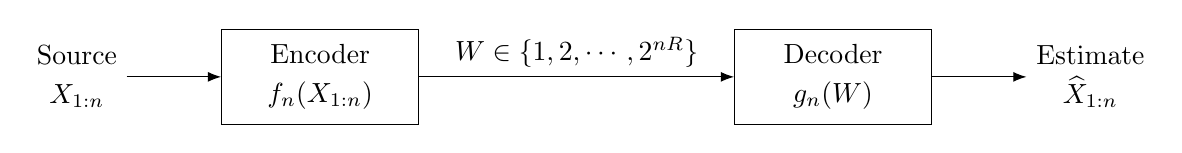
\begin{tikzpicture}[auto, node distance=1.5cm, >=Latex]
	
	% Define nodes
	\node [align=center](message) {Source \\ $X_{1:n}$};
	\node [draw, rectangle, right=1.2cm of message, minimum width=2.5cm, minimum height=1.2cm, align=center] (encoder) {Encoder \\ $f_n(X_{1:n})$};
	\node [draw, rectangle, right=4cm of encoder, minimum width=2.5cm, minimum height=1.2cm, align=center] (decoder) {Decoder \\ $g_n(W)$};
	\node [right=1.2cm of decoder, align=center] (estimate) {Estimate \\ $\widehat{X}_{1:n}$};
	
	% Arrows between blocks with labels
	\draw[->] (message) -- (encoder);
	\draw[->] (encoder) -- (decoder) node[midway, above] {$W\in\{1,2,\cdots,2^{nR}\}$};
	\draw[->] (decoder) -- (estimate);
\end{tikzpicture}
\end{center}
\vspace{0.3cm}
\begin{itemize}
\item The source produces a sequence $X_1, X_2, \cdots$ of i.i.d. random variable with distribution $p(x)$ supported on a possibly infinite alphabet $\cal{X}$.
\item The encoder is a mapping $f_n:\cal{X}^n\to\{1,2,\cdots,2^{nR}\}$ that describes every source sequence by an index $w$. The rate is given by
\begin{align*}
	R=\frac{1}{n}\log_2\left\vert\cal{W}\right\vert. 
\end{align*}
\item The decoder $g_n:\{1,2,\cdots,2^{nR}\}\to\wh{\cal{X}}^n$ maps each index $w$ to an estimate $\hat{x}^n\in\wh{\cal{X}}$, where $\wh{\cal{X}}$ is
a finite reconstruction alphabet.
\end{itemize}
\begin{definition}[Rate measure]
A \textit{per-letter distortion measure} is a mapping $\cal{X}\times\wh{\cal{X}}\to\bbR_+$ from the set of source alphabet-reconstruction pairs into the nonnegative real numbers. The distortion measure is \textit{bounded} if the maximum value of the distortion is finite:
\begin{align*}
	\sup_{x\in\in\cal{X},\wh{x}\in\wh{\cal{X}}}d(x,\hat{x})<\infty.
\end{align*}
The distortion between two sequences $x_{1:n}$ and $\wh{x}_{1:n}$ is given by the average per-letter distortion:
\begin{align*}
	d(x_{1:n},\wh{x}_{1:n})=\frac{1}{n}\sum_{i=1}^n d(x_i,\wh{x}_i).
\end{align*}
\end{definition}
\begin{example} Here are two examples of distortion.
\begin{itemize}
\item[(i)] (Hamming distortion). $d(x,\wh{x})=\mathds{1}_{\{x\neq\wh{x}\}}$. This is often used for discrete alphabets.
\item[(ii)] (Square-error distortion). $d(x,\wh{x})=\vert x-\wh{x}\vert^2$. This is one of the most popular distortion measures used for continuous alphabets.
\end{itemize}
\end{example}
\begin{definition}
A $(2^{nR}, n)$ rate distortion coding scheme consists of
\begin{itemize}
\item a source alphabet $\cal{X}$ and a reconstruction alphabet $\wh{\cal{X}}$,
\item a encoder $f_n:\cal{X}^n\to\{1,2,\cdots,2^{nR}\}$ and a decoder $g_n:\{1,2,\cdots,2^{nR}\}\to\wh{\cal{X}}^n$, and
\item a distortion measure $d:\cal{X}\times\wh{\cal{X}}\to\bbR_+$.
\end{itemize}
The (expected) distortion associated with this coding scheme is defined as
\begin{align*}
	D=\E\left[d(X_{1:n},\wh{X}_{1:n})\right]=\sum_{x_{1:n}\in\cal{X}^n}p(x_{1:n})\,d(x_{1:n},g_n(f_n(x_{1:n})))
\end{align*}
The collection of $n$-tuples $g_n(1),g_n(2),\cdots,g_n(2^{nR})$, denoted by $\wh{X}_{1:n}(1),\wh{X}_{1:n}(2),\cdots,\wh{X}_n(2^{nR})$, constitutes the \textit{codebook}, and $f^{-}_n(1),f^{-1}_n(2),\cdots,f^{-1}_n(2^{nR})$ are the associated \textit{assignment regions}.
\end{definition}
{\bf Remark.}\quad $\wh{X}_{1:n}$ is referred to as the \textit{vector quantization, reconstruction, or estimate} of $X_{1:n}$.
\begin{definition}
We call $(R,D)$ a \textit{rate-distortion pair}.
\begin{itemize}
\item[(i)] A rate-distortion pair $(R,D)$ is said to be \textit{achievable} if
there exists a sequence of $(2^{nR},n)$ rate distortion coding schemes $(f_n,g_n)$ with
\begin{align*}
	\limsup_{n\to\infty}\E\left[d(X_{1:n},\wh{X}_{1:n})\right]\leq D.
\end{align*}
\item[(ii)] The \textit{rate distortion region} for a source is the closure of the set of achievable rate distortion pairs $(R,D)$.
\item[(iii)] The \textit{rate distortion function} $R(D)$ is the infimum of rates $R$ such that $(R,D)$ is in the rate distortion region of the source for a given distortion $D$.
\item[(iv)]  The \textit{distortion rate function} $D(R)$ is the infimum of all distortions $D$ such that $(R,D)$ is in the rate distortion region of the source for a given rate $R$.
\end{itemize}
\end{definition}
\paragraph{Remark.} If the distortion rate is $D=0$, the coding scheme is accurate. According to Shannon's source coding theorem, we require $R=H(X)$. This is not feasible for continuous variable $X$.

\subsection{Information Rate Distortion Function}
\begin{definition}
Let $X$ be a source from a distribution $p(x)$ on $\cal{X}$. The \textit{information rate distortion function} $R^{(I)}(D)$ for a source
$X$ with distortion measure $d$ is defined as
\begin{align*}
	R^{(I)}(D)=\inf_{p(\wh{x}|x):\,\E[d(X,\wh{X})]\leq D} I(X;\wh{X})=\inf_{p(\wh{x}|x):\,\E[d(X,\wh{X})]\leq D} I(p(x),p(\wh{x}|x)).
\end{align*}
Here the infimum is taken over all conditional distributions of $\wh{X}$ given $X$ such that the expected distortion constraint $\E[d(X,\wh{X})]\leq D$ is satisfied.
\end{definition}

We first introduce an important property of rate distortion function $R(D)$, then calculate the information rate distortion function for some sources.
\begin{theorem}\label{rdnonincrconvex}
The information rate distortion function $R^{(I)}(D)$ is a non-increasing convex function of $D$.
\end{theorem}
\begin{proof}
When the distortion $D$ increases, the set of feasible conditional distributions $p(\wh{x}|x)$ is also increasing. Since $R^{(I)}(D)$ is the infimum taken over this set, it is non-increasing.
	
To show the convexity of $R^{(I)}$, take $D_1,D_2>0$ and $\epsilon>0$. Let $\wh{X}_1|X\sim p_1(\wh{x}|x)$ and $\wh{X}_2|X\sim p_2(\wh{x}|x)$ be the conditional distributions such that
\begin{align*}
	I(X;\wh{X}_1)\leq R^{(I)}(D_1)+\epsilon,\quad I(X;\wh{X}_2)\leq R^{(I)}(D_2)+\epsilon.
\end{align*}
For any $\lambda\in[0,1]$, consider the distribution $p_\lambda(\wh{x}|x)=\lambda p_1(\wh{x}|x)+(1-\lambda)p_2(\wh{x}|x)$. The distortion associated to the distribution $p_\lambda(x,\wh{x})=p_\lambda(\wh{x}|x)p(x)$, by linearity of expectation, satisfies
\begin{align*}
	\E\left[d(X,\wh{X})\right]\leq D_\lambda=\lambda D_1+(1-\lambda)D_2.
\end{align*}
By convexity of mutual information,
\begin{align*}
	I(p(x),p_\lambda(\wh{x}|x))\leq\lambda I(p(x),p_1(\wh{x}|x))+(1-\lambda)I(p(x),p_2(\wh{x}|x))\leq \lambda R^{(I)}(D_1)+(1-\lambda)R^{(I)}(D_2)+\epsilon.
\end{align*}
Since $R^{(I)}(D_\lambda)$ is no greater than the last display, and $\epsilon>0$ is arbitrarily taken, we have
\begin{align*}
	R^{(I)}(D_\lambda)\leq \lambda R^{(I)}(D_1)+(1-\lambda)R^{(I)}(D_2)
\end{align*}
Thus we complete the proof.
\end{proof}

\begin{example}[Binary source with Hamming distortion]
The information rate distortion function for an i.i.d. $X\sim\mathrm{Bernoulli}(p)$ source with Hamming distortion is given by
\begin{align*}
	R^{(I)}(D)=\begin{cases}
		H(p)-H(D), &0\leq D\leq\min\{p,1-p\}\\
		0, &D>\min\{p,1-p\}.
	\end{cases}
\end{align*}
\begin{proof}
Let $\wh{\cal{X}}=\{0,1\}$, and let $p(\wh{x}|x)$ be any distribution satisfying the expected distortion constraint, That is, $\bbP(\wh{X}\neq X)\leq D$. Consider $B=\mathds{1}_{\{\wh{X}\neq X\}}=X+\wh{X}\mod 2$. Then
\begin{align*}
	I(X;\wh{X})&=H(X)-H(X|\wh{X})=H(X)-H(B|\wh{X})\geq H(X)-H(B).
\end{align*}
When $D\leq1/2$, we have $H(B)\leq H(D)$, and $I(X;\wh{X})\geq H(p)-H(D)$; otherwise, we have $D>\min\{p,1-p\}$, and by definition $I(X;\wh{X})\geq 0$. Hence
\begin{align*}
	R^{(I)}(D)\geq\begin{cases}
		H(p)-H(D), &0\leq D\leq\min\{p,1-p\}\\
		0, &D>\min\{p,1-p\}.
	\end{cases}
\end{align*}
It remains to show the opposite inequality. If $p<\frac{1}{2}$ and $D\geq p$, we let $\wh{X}=0$ with probability $1$. Then $\bbP(\wh{X}\neq X)=p\leq D$, and $I(X;\wh{X})=0$. A similar conclusion applies for $p>\frac{1}{2}$ and $D\geq 1-p$. Hence 
\begin{align*}
	R^{(I)}(D)=0,\quad D>\min\{p,1-p\}.
\end{align*}
Now we show the case $0\leq D<\min\{p,1-p\}$. Without loss of generality assume $0\leq D<p\leq\frac{1}{2}$. We consider the joint distribution
\begin{align*}
	&\bbP(X=0,\wh{X}=0)=\frac{(1-D)(1-p-D)}{1-2D},\quad\bbP(X=0,\wh{X}=1)=\frac{D(p-D)}{1-2D},\\
	&\bbP(X=1,\wh{X}=0)=\frac{D(1-p-D)}{1-2D},\quad\bbP(X=1,\wh{X}=1)=\frac{(1-D)(p-D)}{1-2D}.
\end{align*}
This distribution satisfies the expected distortion constraint $\bbP(\wh{X}\neq X)=D$, and
\begin{align*}
	R^{(I)}(D)\leq I(X;\wh{X})=H(X)-H(X|\wh{X})=H(p)-H(D).
\end{align*}
Thus we complete the proof.
\end{proof}
\end{example}

\begin{example}[Gaussian source with square-error distortion]
The information rate distortion function for an i.i.d. $X\sim\cal{N}(0,\sigma^2)$ source with square-error distortion is given by
\begin{align*}
	R^{(I)}(D)=\begin{cases}
		\displaystyle\frac{1}{2}\log\frac{\sigma^2}{D}, &0\leq D\leq\sigma^2\vspace{0.1cm}\\
		0, &D>\sigma^2.
	\end{cases}
\end{align*}
\end{example}
\begin{proof}
Let $(X,\wh{X})$ be distributed such that $X\sim\cal{N}(0,\sigma^2)$ and $\E\left[(X-\wh{X})^2\right]\leq D$. Then
\begin{align*}
	I(X;\wh{X})=h(X)-h(X|\wh{X})=\log(2\pi\e\sigma^2)-h(X-\wh{X}|\wh{X})\geq\log(2\pi\e\sigma^2)-h(X-\wh{X}). 
\end{align*}
By Theorem \ref{gaussmaxdiffent},
\begin{align*}
	h(X-\wh{X})\leq\log\left(2\pi\e\E\left[(X-\wh{X})^2\right]\right)\leq \log(2\pi\e D).
\end{align*}
Hence
\begin{align*}
	R^{(I)}(D)\geq\inf_{p(\wh{x}|x):\,\E[(X-\wh{X})^2]\leq D}I(X;\wh{X})\geq\max\left\{\log\frac{\sigma^2}{D},0\right\}.
\end{align*}
Now we prove the other side. If $D\geq\sigma^2$, we can simply set $\wh{X}=0$, which satisfies the expected distortion constraint $\E[(X-\wh{X})^2]\leq D$. If $D<\sigma^2$, we choose distribution given by the Gaussian kernel
\begin{align*}
	X=\wh{X}+Z,\quad \wh{X}\sim\cal{N}(0,\sigma^2-D)\quad and\quad Z\sim\cal{N}(0,D).
\end{align*}
which also satisfies the expected distortion constraint $\E[(X-\wh{X})^2]=D$ Then
\begin{align*}
	R^{(I)}(D)\geq I(X;\wh{X})=h(X)-h(X|\wh{X})=\log\frac{\sigma^2}{D}.
\end{align*}
Thus we complete the proof.
\end{proof}

\subsection{Rate Distortion Theorem}
The main theorem of rate distortion theory can now be stated as follows:
\begin{theorem}\label{rdthm}
The rate distortion function for an i.i.d. source $X\sim p$ and a \textit{bounded} distortion measure $d:\cal{X}\times\wh{\cal{X}}\to\bbR_+$ is equal to the associated information rate distortion function, i.e.
\begin{align*}
	R(D)=R^{(I)}(D).
\end{align*}
This theorem includes two parts:
\begin{itemize}
	\item (Achievability). If $R>R^{(I)}(D)$, the rate-distortion pair $(R,D)$ is achievable.
	\item (Converse). If the rate-distortion pair $(R,D)$ is achievable, then $R\geq R^{(I)}(D)$.
\end{itemize}
\end{theorem}
\begin{proof}[Proof of Theorem \ref{rdthm} (Converse)]
	For any sequence of $(2^{nR},n)$ coding schemes such that $$\lim_{n\to\infty}\E[d(X_{1:n};\wh{X}_{1:n})]\leq D,$$ we want to show that $R\geq R^{(I)}(D)$. We take $\epsilon>0$, then there exists $N$ such that $\E[d(X_{1:n};\wh{X}_{1:n})]\leq D+\epsilon$ for all $n\geq N$. Since there are $2^{nR}$ values in the range of $f_n$,  
	\begin{align}
		nR\geq H(f_n(X_{1:n}))= H(f_n(X_{1:n}))-H(f_n(X_{1:n})|X_{1:n})=I(X_{1:n};f(X_{1:n}))\label{rtconverse1}
	\end{align}
	By data processing inequality,
	\begin{align}
		I(X_{1:n};f(X_{1:n}))&\geq I(X_{1:n};\wh{X}_{1:n})=H(X_{1:n})-H(X_{1:n}|\wh{X}_{1:n})\notag\\
		&=\sum_{i=1}^n H(X_i)-H(X_{1:n}|\wh{X}_{1:n})\tag{By independence of $X_{1:n}$}\\
		&=\sum_{i=1}^n H(X_i)-\sum_{i=1}^nH(X_i|X_{i-1},\cdots,X_1,\wh{X}_{1:n})\tag{By the chain rule}\\
		&\geq\sum_{i=1}^n H(X_i)-\sum_{i=1}^nH(X_i|\wh{X}_i)\tag{Conditioning does not increase entropy}\\
		&=\sum_{i=1}^n I(X_i;\wh{X}_i).\label{rtconverse2}
	\end{align}
	By definition of the information distortion function $R^{(I)}(D)$, 
	\begin{align*}
		I(X_i;\wh{X}_i)\geq R^{(I)}\left(\E\left[d(X_i;\wh{X}_i)\right]\right).
	\end{align*}
	By convexity of $R^{(I)}(D)$ and Jensen's inequality, we get
	\begin{align}
		\sum_{i=1}^n I(X_i;\wh{X}_i)\geq\sum_{i=1}^n R^{(I)}\left(\E\left[d(X_i;\wh{X}_i)\right]\right)\geq nR^{(I)}\left(\frac{1}{n}\sum_{i=1}^n\E\left[d(X_i;\wh{X}_i)\right]\right)=nR^{(I)}\left(\E\left[d(X_{1:n};\wh{X}_{1:n})\right]\right).\label{rtconverse3}
	\end{align}
	Combining (\ref{rtconverse1}), (\ref{rtconverse2}) and (\ref{rtconverse3}), we obtain
	\begin{align*}
		R\geq R^{(I)}\left(\E\left[d(X_{1:n};\wh{X}_{1:n})\right]\right)\geq R^{(I)}(D+\epsilon).
	\end{align*}
This inequality holds for all $\epsilon>0$. Since the function $R^{(I)}(D)$ is convex, it is continuous, and
\begin{align*}
	R\geq\lim_{\epsilon\downarrow 0}R^{(I)}(D+\epsilon)=R^{(I)}(D).
\end{align*}
Thus we complete the proof.
\end{proof}
\begin{definition}[Distortion $\epsilon$-typical set]

\end{definition}
\begin{proof}[Proof of Theorem \ref{rdthm} (Achievability)]

\end{proof}


\newpage
\section{$f$-Divergences}
\subsection{Definition and Properties}
\begin{definition}[$f$-divergence]\label{fdivdef}
Let $P$ and $Q$ be two probability measures on a measurable space $(\mathcal{X},\mathscr{F})$. For any convex function $f:[0,\infty)\to(-\infty,\infty]$ such that (i) $f(1)=0$,  (ii) $f$ is strictly convex at $1$,\footnote{By strict convexity at $1$, we mean that for all $x,y\in(0,\infty)$ and $0<\lambda<1$ such that $\lambda x+(1-\lambda)y=1$, we have $$\lambda f(x)+(1-\lambda)f(y)>f(1).$$ For a random variable $X$ with $\E[X]=1$, the Jensen's inequality $\E[f(X)]\geq f(\E[X])$ is strict if $X$ is not a constant.} and (iii) $f$ is finite except possibly at 0,
the $f$-divergence of $Q$ with respect to $P$ is defined as follows:
\begin{itemize}
\item[(i)] If $Q\ll P$, 
	\begin{align*}
		D_f(Q\Vert P) := \int f\left(\frac{dQ}{dP}\right)\,dP,
	\end{align*}
where the notation $\frac{dQ}{dP}$ stands for the Radon-Nikodym derivative of $Q$ with respect to $P$.
\item[(ii)] More generally, let $\mu$ be any dominating measure of $P$ and $Q$, i.e. $P\ll\mu$ and $Q\ll\mu$. Assume $dP=p\,d\mu$ and $dQ=q\,d\mu$. Then
\begin{align}
	D_f(Q\Vert P) := \int_{\{p>0\}} f\left(\frac{q}{p}\right)p\,d\mu+f^\prime(\infty)\,Q\{p=0\},\label{generalfdiv}
\end{align}
where $f^\prime(\infty)=\lim_{x\to 0^+}xf(\frac{1}{x})$.
\end{itemize} 
\end{definition} 

\paragraph{Remark.} In fact, the definition (\ref{generalfdiv}) comes from the following division:
\begin{align*}
	D_f(Q\Vert P)=\int_{\{p>0\}}f\left(\frac{q}{p}\right)\,dP+\int_{\{p=0\}}\frac{p}{q}f\left(\frac{q}{p}\right)\,dQ=\int_{\{p>0\}}f\left(\frac{q}{p}\right)p\,d\mu+\lim_{x\to 0^+}xf\left(\frac{1}{x}\right)Q\{p=0\}.
\end{align*}
In practice, we often use the following two forms of $f$-divergence:
\begin{itemize}
\item When $\mathcal{X}$ is discrete, $P$ and $Q$ are probability mass functions:
\begin{equation*}
	D_f(Q\Vert P) = \sum_{x\in\mathcal{X}}f\left(\frac{Q(x)}{P(x)}\right)P(x)=\E_{P}\left[f\left(\frac{Q}{P}\right)\right].
\end{equation*}
	
\item When $P$ and $Q$ are characterized by density functions $p$ and $q$ (i.e. their Radon-Nikodym derivatives with respect to the Lebesgue measure), respectively, then
\begin{equation*}
	D_f(q\Vert p) = \int f\left(\frac{q(x)}{p(x)}\right)p(x)\,dx=\E_{X\sim p}\left[f\left(\frac{p(X)}{q(X)}\right)\right].
\end{equation*}
\end{itemize}
We use the convention that
\begin{itemize}
\item $f(0)=f(0^+)$,
\item $0f\left(\frac{0}{0}\right)=0$, and
\item $0f\left(\frac{a}{0}\right)=\lim_{x\to 0^+}xf\left(\frac{a}{x}\right)=af^\prime(\infty)$.
\end{itemize}
Furthermore, by definition, if $P\perp Q$,
\begin{align*}
	D_f(Q\Vert P)=f(0)+f^\prime(\infty)=\lim_{x\to 0^+}\left[(1-x)f\left(\frac{x}{1-x}\right)+xf\left(\frac{1}{x}\right)\right]>\lim_{x\to 0^+}f\left(x+1\right)=f(1)=0.
\end{align*}
An $f$-divergence provide an evaluation of the difference between two probability distributions.

\begin{proposition}[Positive-definiteness of $f$-divergence]
Let $D_f$ be an $f$-divergence. Then $$D_f(Q\Vert P) \geq 0,$$ and the equality holds if and only if $P=Q$.
\end{proposition}
\begin{proof}
From Jensen's inequality, the convexity of $f$ implies:
\begin{align*}
	D_f(Q\Vert P) &= \mathbb{E}_P\left[f\left(\frac{Q}{P}\right)\right] \geq f\left(\mathbb{E}_P\left[\frac{Q}{P}\right]\right) = f(1) = 0.
\end{align*}
By the strict convexity of $f$ at $1$, the equality holds if and only if $P=Q.$
\end{proof}

\begin{definition}[Examples of $f$-divergence]\label{fdivex}
The following are some commonly used $f$-divergences:
\begin{itemize}
	\item[(i)] Total variation distance. $f(x)=\frac{1}{2}\vert x-1\vert:$
	\begin{equation*}
		d_{\mathrm{TV}}(P,Q) = \frac{1}{2}\E_P\left[\left\vert\frac{Q}{P} - 1\right\vert\right] = \frac{1}{2}\int\vert dQ - dP\vert.\label{eq:3.4}
	\end{equation*}
	Clearly, we have $d_\mathrm{TV}(P,Q) = d_\mathrm{TV}(Q,P)$. Furthermore, the triangle inequality follows from definition:
	\begin{align*}
		d_\mathrm{TV}(P,Q)\leq d_\mathrm{TV}(P,R)+d_\mathrm{TV}(R,Q).
	\end{align*} 
Therefore, the total variation distance is a metric on the space of all probability measures on $(\cal{X},\Sigma)$.
	\item[(ii)] Kullback-Leibler divergence. $f(x) = x\log x:$
	\begin{equation*}
		D(Q\Vert P) = \E_P\left[\frac{Q}{P}\log\left(\frac{Q}{P}\right)\right]=\E_Q\left[\log\left(\frac{Q}{P}\right)\right]. \label{eq:3.5}
	\end{equation*}
	\item[(iii)] Pearson $\chi^2$-divergence. $f(x) = x^2-1:$
\begin{equation*}
	\chi^2(Q\Vert P) = \int\frac{Q^2}{P} - 1=\int\frac{(P-Q)^2}{P}. \label{eq:3.7}
\end{equation*}
	\item[(iv)] Squared Hellinger distance.  $f(x) = \frac{1}{2}(1-\sqrt{x})^2:$
	\begin{equation*}
		H^2(P,Q) = \frac{1}{2}\E_P\left[\biggl(1-\sqrt{\frac{Q}{P}}\biggr)^2\right] = \frac{1}{2}\int\left(\sqrt{P} - \sqrt{Q}\right)^2. \label{eq:3.6}
	\end{equation*}
	Clearly, we have $H^2(P,Q) = H^2(Q,P)$. We further define the Hellinger distance $H(P,Q)=\sqrt{H^2(P,Q)}$. Then the triangle inequality $H(P,Q)\leq H(P,R)+H(R,Q)$ follows from the case for $L^2$-norm. Therefore, the Hellinger distance $H(\cdot,\cdot)$ is a metric on the space of all probability measures on $(\cal{X},\Sigma)$.
	\item[(v)] Jensen-Shannon divergence. $f(x) = \frac{x}{2}\log x - \frac{1+x}{2}\log\left(\frac{1+x}{2}\right):$
	\begin{equation*}
		D_{\mathrm{JS}}(P,Q) = \frac{1}{2}D(P\Vert M) + \frac{1}{2}D(Q\Vert M),\label{eq:3.8}
	\end{equation*}
	where $M=\frac{1}{2}P+\frac{1}{2}Q.$ This is also known as the symmetrized Kullback-Leibler divergence.
	\item[(vi)] Le Cam distance. $f(x)=\frac{(1-x)^2}{2(1+x)}:$
	\begin{align*}
		\Le(P,Q)=\frac{1}{2}\int\frac{(P-Q)^2}{P+Q}.
	\end{align*}
\end{itemize}
\end{definition} 
Now we discuss more properties of $f$-divergences.

\begin{proposition}[Properties of $f$-divergences] Let $D_f$ be an $f$-divergence.
\begin{itemize}
\item[(i)] (Monotonicity). Let $P_{X,Y}$ and $Q_{X,Y}$ be two joint distributions of random variables $X$ and $Y$. Then
\begin{align*}
	\max\left\{D_f(Q_X\Vert P_X),D_f(Q_Y\Vert P_Y)\right\}\leq D_f(Q_{XY}\Vert P_{XY}).
\end{align*}
\item[(ii)] (Data processing inequality). Fix the conditional distribution $P_{Y|X}$ of $Y$ given $X$. Let $P_{X,Y}=P_XP_{Y|X}$ and $Q_{X,Y}=Q_XP_{Y|X}$. Then
\begin{align*}
	D_f(Q_Y\Vert P_Y) \leq D_f(Q_X\Vert P_X).
\end{align*}
\item[(iii)] (Joint convexity). The mapping $(Q,P)\mapsto D_f(Q\Vert P)$ is jointly convex. That is, for any distributions $P_1,P_2,Q_1,Q_2$ and any $0\leq\lambda\leq 1$,
\begin{align*}
	D_f\left(\lambda Q_1+(1-\lambda)Q_2\Vert\lambda P_1+(1-\lambda)P_2\right)\leq\lambda D_f(Q_1\Vert P_1)+(1-\lambda)D_f(Q_2\Vert P_2).
\end{align*}
\item[(iv)] (Conditional increment). Given two conditional distributions $P_{Y|X}$ and $Q_{Y|X}$ and a marginal distribution $P_X$, define the conditional $f$-divergence:
\begin{align*}
	D_f(Q_{Y|X}\Vert P_{Y|X}|P_X) &:=\int_{\cal{X}} D_f(Q_{Y|X=x}\Vert P_{Y|X=x})\,dP(x)= \mathbb{E}_{X\sim P_X}\left[D_f(Q_{Y|X}\Vert P_{Y|X})\right].
\end{align*}
Let $P_{X,Y}=P_XP_{Y|X}$ and $Q_{X,Y}=P_XQ_{Y|X}$. Then
\begin{align*}
	D_f(Q_Y\Vert P_Y) &\leq D_f(Q_{Y|X}\Vert P_{Y|X}|P_X).
\end{align*}
\end{itemize}
\end{proposition}
\begin{proof}
(i) Using Jensen's inequality:
\begin{align*}
	D_f(Q_{X,Y}\Vert P_{X,Y})&=\E_{P_{X,Y}}\left[f\left(\frac{Q_{X,Y}}{P_{X,Y}}\right)\right]=\E_{P_X}\left[\E_{P_{Y|X}}\left[f\left(\frac{Q_{X,Y}}{P_{X,Y}}\right)\right]\right]\\
	&\geq\E_{P_X}\left[f\left(\E_{P_{Y|X}}\left[\frac{Q_{X}}{P_{X}}\frac{Q_{Y|X}}{P_{Y|X}}\right]\right)\right]\\
	&=\E_{P_X}\left[f\left(\frac{Q_{X}}{P_{X}}\E_{P_{Y|X}}\left[\frac{Q_{Y|X}}{P_{Y|X}}\right]\right)\right]\\
	&=\E_{P_X}\left[f\left(\frac{Q_{X}}{P_{X}}\right)\right]\\
	&=D_f(Q_X\Vert P_X).
\end{align*}
Switching $X$ and $Y$ yields $D_f(Q_{X,Y}\Vert P_{X,Y})\geq D_f(Q_Y\Vert P_Y)$.\vspace{0.12cm}

(ii) Following that (i), it suffices to show $D_f(Q_X\Vert P_X)=D_f(Q_{X,Y}\Vert P_{X,Y})$. This is true since the conditional distribution $P_{Y|X}$ is fixed:
\begin{align*}
	D_f(Q_{X,Y}\Vert P_{X,Y})&=\E_{P_{X,Y}}\left[f\left(\frac{Q_{X,Y}}{P_{X,Y}}\right)\right]=\E_{P_{X,Y}}\left[f\left(\frac{Q_{X}}{P_{X}}\right)\right]\\
	&=\E_{P_X}\left[f\left(\frac{Q_{X}}{P_{X}}\right)\right]=D_f(Q_X\Vert P_X).
\end{align*}

(iii) Fix $\lambda\in[0,1]$, and let $B\sim\mathrm{Bernoulli}(\lambda)$. We set $P_{X|B=1}=P_1$, $P_{X|B=0}=P_2$, and $Q_{X|B_1}=Q_1$ and $Q_{X|B=0}=Q_2$. Since the distribution $P_X$ of $X$ is fixed,
\begin{align*}
	\frac{Q_{X,B}}{P_{X,B}}=\frac{Q_B}{P_B}\frac{Q_{X|B}}{P_{X|B}}=\frac{Q_{X|B}}{P_{X|B}}.
\end{align*}
Then
\begin{align*}
	D_f(Q_{X,B}\Vert P_{X,B})=\E_{P_B}\left[\E_{P_{X|B}}\left[ f\left(\frac{Q_{X|B}}{P_{X|B}}\right)\right]\right]=\lambda D_f(Q_1\Vert P_1)+(1-\lambda)D_f(Q_2\Vert P_2).
\end{align*}
On the other hand, the monotonicity implies
\begin{align*}
	D_f(Q_{X,B}\Vert P_{X,B})\geq D_f(Q_X\Vert P_X)=D_f\left(\lambda Q_1+(1-\lambda)Q_2\Vert\lambda P_1+(1-\lambda)P_2\right).
\end{align*}
Combining the last two displays gives the wanted result.\vspace{0.12cm}

(iv) By calculus, the marginal distributions of $Y$ are given by
\begin{align*}
	Q_Y=\int_{\cal{X}} Q_{Y|X=x}\,dP_X(x)=\E_{X\sim P_X}[Q_{Y|X}],\quad P_Y=\int_{\cal{X}} P_{Y|X=x}\,dP_X(x)=\E_{X\sim P_X}[P_{Y|X}].
\end{align*}
Then by joint convexity of $D_f(\cdot\Vert\cdot)$ and Jensen's inequality,
\begin{align*}
	D_f(Q_{Y|X}\Vert P_{Y|X}|P_X)=\mathbb{E}_{X\sim P_X}\left[D_f(Q_{Y|X}\Vert P_{Y|X})\right]\geq D_f\left(\mathbb{E}_{X\sim P_X}[Q_{Y|X}]\,\Vert\,\mathbb{E}_{X\sim P_X}[P_{Y|X}]\right)=D_f(Q_Y\Vert P_Y).
\end{align*}
Thus we complete the proof.
\end{proof}
The data processing inequality for $f$-divergence has many applications. Here are some basic examples.
\begin{proposition}\label{dataproconseq}
Let $P$ and $Q$ be two probability measures on $(\cal{X},\mathscr{F})$, and let $A\in\mathscr{F}$.
\begin{itemize}
\item[(i)] $\vert P(A)-Q(A)\vert\leq d_\mathrm{TV}(P,Q)$. \quad (ii) $\vert\sqrt{P(A)}-\sqrt{Q(A)}\vert\leq\sqrt{2}H(P,Q)$.
\item[(iii)] $\vert P(A)-Q(A)\vert^2\leq\chi^2(Q\Vert P)P(A)(1-P(A))$.
\item[(iv)] $Q(A)\log\frac{1}{P(A)}\leq D(Q\Vert P)+\log 2$.
\end{itemize}
\end{proposition}
\begin{proof}
We fix $X\sim P_X=P$ or $X\sim Q_X=Q$, and define $Y=\mathds{1}_{\{X\in A\}}$. Then $P_Y=\mathrm{Bernoulli}(P(A))$, and $Q_Y=\mathrm{Bernoulli}(Q(A))$. Use the data processing inequality:
\begin{align*}
	D_f(Q_Y\Vert P_Y)\leq D_f(Q_X\Vert P_X)=D_f(Q\Vert P).
\end{align*}
\begin{itemize}
\item[(i)] Since $d_\mathrm{TV}(P_Y,Q_Y)=\frac{1}{2}\vert Q(A)-P(A)\vert+\frac{1}{2}\vert 1-Q(A)-(1-P(A))\vert=\vert Q(A)-P(A)\vert$, we have
\begin{align*}
	\vert P(A)-Q(A)\vert\leq d_\mathrm{TV}(P,Q).
\end{align*}
\item[(ii)] By definition,
\begin{align*}
	H^2(P_Y,Q_Y)&=\frac{1}{2}\left(\sqrt{P(A)}-\sqrt{Q(A)}\right)^2+\frac{1}{2}\left(\sqrt{1-P(A)}-\sqrt{1-Q(A)}\right)^2.
\end{align*}
Hence
\begin{align*}
	\frac{1}{2}\left(\sqrt{P(A)}-\sqrt{Q(A)}\right)^2\leq H^2(P_Y,Q_Y)\leq H^2(P,Q).
\end{align*}
\item[(iii)] By definition, $$\chi^2(Q_Y\Vert P_Y)=\frac{\vert Q(A)-P(A)\vert^2}{P(A)}+\frac{\vert 1-Q(A)-(1-P(A))\vert^2}{1-P(A)}=\frac{\vert Q(A)-P(A)\vert^2}{P(A)(1-P(A))}$$
Hence
\begin{align*}
	\vert Q(A)-P(A)\vert\leq\chi^2(Q\Vert P)P(A)(1-P(A)).
\end{align*}
\item[(iv)] By definition,
\begin{align*}
	D(Q_Y\Vert P_Y)&=Q(A)\log\frac{Q(A)}{P(A)}+(1-Q(A))\log\frac{1-Q(A)}{1-P(A)}\\
	&\geq Q(A)\log\frac{1}{P(A)}+(1-Q(A))\log\frac{1}{1-P(A)}-\log 2.
\end{align*}
Hence
\begin{align*}
	Q(A)\log\frac{1}{P(A)}\leq D(Q\Vert P)+\log 2.
\end{align*}
Thus we conclude the proof.
\end{itemize}
\end{proof}

In fact, the first inequality in the above proposition can become equality.
\begin{proposition}\label{tvrepsup}
Let $P$ and $Q$ be two probability measures on $(\cal{X},\mathscr{F})$. Then
\begin{align*}
d_\mathrm{TV}(P,Q)=\sup_{A\in\mathscr{F}}P(A)-Q(A).	
\end{align*}
\end{proposition}
\begin{proof}
We consider the signed measure $\mu=P-Q$. By Hahn decomposition theorem, there exists a partition $\mathcal{X}=\mathcal{P}\cap\mathcal{N}$ such that
\begin{itemize}
\item[(i)] $\mathcal{P},\mathcal{N}\in\mathscr{F}$ and $\mathcal{P}\cap\mathcal{N}=\emptyset$, 
\item[(ii)] $P(A\cap\mathcal{P})-Q(A\cap\mathcal{P})\geq 0$ for all $A\in\mathscr{F}$, and 
\item[(iii)] $P(A\cap\mathcal{P})-Q(A\cap\mathcal{P})\leq 0$ for all $A\in\mathscr{F}$.
\end{itemize}
We take $A=\mathcal{P}$. Then
\begin{align*}
	d_{\mathrm{TV}}(P,Q)&=\frac{1}{2}\int_{\cal{P}}[dP-dQ]+\frac{1}{2}\int_{\cal{N}}[dQ-dP]\\
	&=\int_{\cal{P}}[dP-dQ]=P(A)-Q(A).
\end{align*}
The conclusion then follows from Proposition \ref{dataproconseq}(i).
\end{proof}

\subsection{Variational Representation}
\begin{definition}[Fenchel conjugate] Let $(\mathcal{X},\langle\cdot,\cdot\rangle)$ be a real Hilbert space, and let $f:\mathcal{X}\to(-\infty,+\infty]$ be a proper function, that is, $\mathrm{dom}(f):=\{x\in\mathcal{X}:f(x)\in\mathbb{R}\}\neq\emptyset.$
The Fenchel conjugate of $f$ is defined as
\begin{equation}
	f^*(t) = \sup_{x\in\mathcal{X}} \{\langle x,t\rangle - f(x)\},\ t\in\mathcal{X}.\label{fencheldual}
\end{equation}
\end{definition}

\paragraph{Remark.} It can be seen that $f^*$ is the pointwise supremum of a collection of affine functions, hence $f^*$ is convex, regardless of $f$ is convex or not. Moreover, it can be shown that the duality $(f^*)^*=f$ holds if $f$ is convex and lower semicontinuous. Below is an immediate consequence of this definition. 

\begin{proposition}[Fenchel-Young inequality]
For all $x,t\in\mathcal{X},$
\begin{equation*}
	f(x) + f^*(t)\geq \langle x,t\rangle.
\end{equation*}
\end{proposition} 

\paragraph{Remark.} Recall that in Definition \ref{fdivdef}, $f$ is defined on $[0,+\infty)$. We complete $f$ by redefining $f(x)=\infty$ for $x<0$, which preserves the convexity of $f$. Moreover, the Fenchel conjugate of $f:\mathbb{R}\to(-\infty,+\infty]$ is well defined: $f^*(t) = \sup_{x\in\mathbb{R}}\{tx - f(x)\},\ t\in\mathbb{R}$. The $f$-divergence admits the following variational representation.

\begin{lemma}[Variational representation of $f$-divergence]
Denote $\mathcal{M}$ by the class of measurable functions on $(\mathcal{X},\Sigma).$ Then the $f$-divergence can be represented as
\begin{equation}
	D_f(Q\Vert P) = \sup_{g\in\mathcal{M}} \left\{\int g\,dQ - \int (f^*\circ g)\,dP \right\}=\sup_{g\in\mathcal{M}} \bigl\{\E_Q[g(X)] - \E_P[f^*(g(X))]\bigr\}.\label{fdivvar}
\end{equation}
Where $f^*$ is the Fenchel conjugate of $f$. If $f$ is differentiable, the supremum is reached at $g = f'(\frac{dQ}{dP})$.
\end{lemma} 
\begin{proof}
We fix the measurable function $g\in\mathcal{M}.$ By Fenchel's duality, we have
\begin{equation*}
	g(x)\frac{Q(x)}{P(x)} - f\left(\frac{Q(x)}{P(x)}\right)\leq f^*(g(x)).
\end{equation*}
Take integration with respect to $P$ on both sides of the equation above, we have
\begin{equation*}
	\int g(x)\,dQ(x) - D_f(Q\Vert P) \leq \int f^*(g(x))\,dP(x).
\end{equation*}
Since $g$ is arbitrarily chosen, we immediately conclude the equality (\ref{fdivvar}). The supremum can be found when the derivative of (\ref{fencheldual}) vanishes.
\end{proof}

\begin{proposition} We provide the variational form of $f$-divergences in Definition \ref{fdivex}.
\begin{itemize}
	\item Total variation distance. $f^*(t) = \begin{cases}
		t,\ \vert t\vert\leq 1/2\\
		\infty,\ \vert t\vert > 1/2
	\end{cases}:$
	\begin{equation*}
		d_\mathrm{TV}(P,Q) = \frac{1}{2}\sup_{\Vert g\Vert_\infty \leq 1} \left(\int g\,dP-\int g\,dQ\right)
	\end{equation*}
	\item Kullback-Leibler divergence. $f^*(t) = \mathrm{e}^{t
		-1}:$
	\begin{equation*}
		D(Q\Vert P) = \sup_{g\in\mathcal{M}} \left\{\int g(x)\,dQ(x) - \int\e^{g(x)-1}\,dP(x)\right\}.
	\end{equation*}
	\item Squared Hellinger distance. $f^*(t)=\begin{cases}\frac{t}{1-2t},\ t<1/2\\
		\infty,\ t\geq 1/2\end{cases}:$
	\begin{equation*}
		H^2(P,Q) = \inf_{g<\frac{1}{2}}\left\{\int g\,dQ - \int \frac{g}{1-2g}\,dP\right\}=\inf_{h<1}\frac{1}{2}\left(\int h\,dQ - \int \frac{h}{1-h}\,dP\right).
	\end{equation*}
\item Jensen-Shannon divergence. $f^*(t) = \begin{cases}
	-\frac{1}{2}\log(2-\mathrm{e}^{2t}),\ t<\frac{1}{2}\log 2\\
	\infty,\ t \geq \frac{1}{2}\log 2.
\end{cases}$:
\begin{align*}
	D_{\mathrm{JS}}(P,Q) &= \sup_{g\leq\frac{1}{2}\log 2} \left\{\int g\,dQ +\frac{1}{2}\int \log(2-\e^{2g})\,dP\right\}\\
	&= \frac{1}{2}\sup_{\Vert h\Vert_\infty < 1} \left\{\int\log(1+h)\,dQ + \int \log(1-h)\,dP\right\}.\tag{$h=\e^{2g}-1$}
\end{align*}
	\item Pearson $\chi^2$-divergence.
	$f^*(t) = \frac{1}{4}t^2 + 1$:
	\begin{equation}
		\chi^2(Q\Vert P) = \sup_{g\in\mathcal{M}}\left\{\int g\,dQ - \frac{1}{4}\int g^2\,dP - 1\right\}.\label{pearsonvar}
	\end{equation}
	Let $g = a+bh,$ and solve (\ref{pearsonvar}) with respect to $a,b$, we obtain a more symmetric version which is directly related to the bias-variance tradeoff:
	\begin{align*}
		\chi^2(Q\Vert P) &=\sup_{h\in\mathcal{M}}\sup_{a,b\in\bbR}\left\{a-\frac{a^2}{4}+b\int h\,dQ -\frac{ab}{2}\int h\,dP-\frac{b^2}{4}\int h^2\,dP - 1\right\}\\
		&=\sup_{h\in\mathcal{M}}\sup_{a\in\bbR}\left\{\frac{\left(a\int h\,dP-2\int h\,dQ\right)^2}{4\int h^2\,dP}-\left(1-\frac{a}{2}\right)^2\right\}\tag*{$\displaystyle\biggl(\text{take}\ b=\frac{a\int h\,dP-2\int h\,dQ}{\int h^2\,dP}\biggr)$}\\
		&= \sup_{h:\mathcal{X}\to\mathbb{R}}\frac{\left(\int h\,dQ-\int h\,dP\right)^2}{\int h^2\,dP - \left(\int h\,dP\right)^2}.\tag*{$\displaystyle\biggl(\text{take}\ a=\frac{2\int h^2\,dP-2\int h\,dP\int h\,dQ}{\int h^2\,dP-(\int h\,dP)^2}\biggr)$}
	\end{align*}
We can write this equality to the expectation form:
\begin{align}
	\chi^2(Q\Vert P)=\sup_{h:\mathcal{X}\to\mathbb{R}}\frac{\left(\E_Q[h(X)]-\E_P[h(X)]\right)^2}{\var_P(h(X))}\label{chisqdivvarrep}
\end{align}
This bound extremely useful later.
\end{itemize}
\end{proposition}

\begin{theorem}[Donsker-Varadhan]
\end{theorem}


\subsection{Inequality between $f$-Divergences and Joint Range}
\begin{theorem}
For two probability measures $P$ and $Q$ on a measurable space $(\mathcal{X},\mathscr{F})$,
\begin{align}\label{chisqklineq}
	D(Q\Vert P)\leq \log\left(1+\chi^2(Q\Vert P)\right).
\end{align}
\end{theorem}
\begin{proof}
By Jensen's inequality,
\begin{align*}
\log\left(1+\chi^2(Q\Vert P)\right)=\log\left(\int\frac{Q^2}{P}\right)\geq\int Q\log\frac{Q}{P}=D(Q\Vert P).
\end{align*}
Thus we complete the proof.
\end{proof}

\begin{theorem}[Pinsker's inequality] 
For two probability measures $P$ and $Q$ on a measurable space $(\mathcal{X},\mathscr{F})$,
\begin{equation*}
	d_{\mathrm{TV}}(P,Q) \leq \sqrt{\frac{1}{2}D(Q\Vert P)}.\label{eq:3.18}
\end{equation*}
\end{theorem}
\begin{proof}
We first consider the case $P=\mathrm{Bernoulli}(p)$ and $Q=\mathrm{Bernoulli}(q)$ with $p\leq q$. Then
\begin{align*}
	D(Q\Vert P)&=q\log\frac{q}{p}+(1-q)\log\frac{1-q}{1-p}\\
	&=q\int_p^q\frac{dt}{t}-(1-q)\int_p^q\frac{dt}{1-t}\\
	&=\int_p^q\frac{q-t}{t(1-t)}\,dt\geq 4\int_p^q(q-t)\,dt=2(q-p)^2.
\end{align*}
Since $d_\mathrm{TV}(P,Q)=q-p$, the inequality follows. For the general case, we take $A\in\mathscr{F}$. Let $P_A=\mathrm{Bernoulli}(P(A))$ be the distribution of the variable $\mathds{1}_{\{X\in A\}}$ under $X\sim P$, and we define $Q_A=\mathrm{Bernoulli}(Q(A))$ similarly. Using the conclusion above and the data processing inequality,
\begin{align*} 
	\vert P(A)-Q(A)\vert = d_{\mathrm{TV}}(P_A,Q_A)\leq\sqrt{\frac{1}{2}D(Q_A\Vert P_A)}\leq\sqrt{\frac{1}{2}D(Q\Vert P)}.
\end{align*}
Taking the supremum $d_\mathrm{TV}(P,Q)=\sup_{A\in\scr{F}}\vert P(A)-Q(A)\vert$, we have the desired result.
\end{proof}

A refinement of Pinsker's inequality is presented below.
\begin{theorem}[Bretagnolle-Huber] 
For two probability measures $P$ and $Q$ on a measurable space $(\mathcal{X},\mathscr{F})$,
\begin{equation*}
	d_{\mathrm{TV}}(P,Q) \leq \sqrt{1 - \e^{-D(Q\Vert P)}} \leq 1 - \frac{1}{2} \e^{-D(Q\Vert P)}.
\end{equation*}
\end{theorem}
\begin{proof}
Similar to the proof of Pinsker's inequality, it suffices to show the Bernoulli case. Let $P=\mathrm{Bernoulli}(p)$ and $Q=\mathrm{Bernoulli}(q)$ with $p\leq q$. Then
\begin{align*}
	D(Q\Vert P)&=q\log\frac{q}{p}+(1-q)\log\frac{1-q}{1-p}\\
	&=-2q\log\sqrt{p}{q}-2(1-q)\log\frac{1-p}{1-q}\\
	&\geq -2\log\left(\sqrt{pq}+\sqrt{(1-p)(1-q)}\right).
\end{align*}
Hence
\begin{align*}
	\e^{-D(Q\Vert P)}&\leq \left(\sqrt{pq}+\sqrt{(1-p)(1-q)}\right)^2\\
	&\leq \left(\sqrt{pq}+\sqrt{(1-p)(1-q)}\right)^2+\left(\sqrt{p(1-p)}-\sqrt{(1-q)q}\right)^2\\
	&=1-(q-p)^2=1-d_\mathrm{TV}(P,Q)^2.
\end{align*}
The desired bound then follows.
\end{proof}

The downside of ad hoc approaches is that it is hard to tell whether those inequalities can be improved or not. However, the key step when we proved the Pinksers inequality, reduction to the case for Bernoulli random variables, is inspiring: is it possible to reduce inequalities between any two $f$-divergences to the binary case?

The joint range of $f$-divergences provides a systematic approach to find inequalities between $f$-divergences.
\begin{definition}[Joint range]\label{jrdef}
Consider two $f$-divergences $D_f$ and $D_g$. The joint
range between $D_f$ and $D_g$ is a subset of $\bbR^2_+$ defined by
\begin{align*}
\cal{R}&=\left\{(D_f(Q\Vert P), D_g(Q\Vert P)): P\ and\ Q\ are\ probability\ measures\ on\ some\ measure\ space\right\},\\
\cal{R}_k&=\left\{(D_f(Q\Vert P), D_g(Q\Vert P)): P\ and\ Q\ are\ probability\ measures\ on\ \{1,2,\cdots,k\}\right\},\quad k=2,3,\cdots.
\end{align*}
\end{definition}
If we know the region $\cal{R}$, we can find a tight inequality between $D_f$ and $D_g$:
\begin{align*}
	D_g(Q\Vert P)\geq F(D_f(Q\Vert P)),
\end{align*}
where $F$ is the lower boundary of $\cal{R}$:
\begin{align*}
	F(t):=\inf\left\{x\geq 0:(t,x)\in\cal{R}\right\}=\inf_{(P,Q):D_f(P\Vert Q)=t}D_g(P\Vert Q),\quad t\geq 0.
\end{align*}

The region $\cal{R}$ seems difficult to characterize since we need to consider probability measures $P$ and $Q$ over all measurable spaces. On the other hand, the region $R_k$ for small $k$ is easy to obtain. The main theorem we will prove is the following, which provides a simple characterization of $\cal{R}$.


\begin{theorem}[Harremoës-Vajda]\label{jrconvjr2}
Given two $f$-divergences $D_f$ and $D_g$, their joint range satisfies
\begin{align*}
	\cal{R}=\conv(\cal{R}_2).
\end{align*}
\end{theorem}
\newpage
The proof of this theorem requires some technical lemmata.
\begin{lemma}\label{repjr}
Given two $f$-divergences $D_f$ and $D_g$, their joint range is
\begin{align}
\cal{R}=\left\{\begin{pmatrix}
\E[f(X)]+f^\prime(\infty)(1-\E[X])\\
\E[g(X)]+g^\prime(\infty)(1-\E[X])
\end{pmatrix}:X\ is\ a\ random\ variable\ with\ X\geq 0\ and\ \E[X]\leq 1\right\}.
\end{align}
Furthermore, for any integer $k$ greater than $1$,
\begin{align}
\cal{R}_k
&=\left\{\begin{pmatrix}
	\E[f(X)]+f^\prime(\infty)(1-\E[X])\\
	\E[g(X)]+g^\prime(\infty)(1-\E[X])
\end{pmatrix}:\ \begin{matrix}
X\ takes\ at\ most\ k-1\ values,\ X\geq 0\ and\ \E[X]\leq 1\\
\ or\ X\ takes\ at\ most\ k\ values,\ X\geq 0\ and\ \E[X]= 1
\end{matrix}\right\}.
\end{align}
\end{lemma}
\begin{proof}
Given any pair of distributions $(P,Q)$ that produces a point of $\cal{R}$, let $p,q$ denote the densities of $P,Q$ under some dominating measure $\mu$, respectively. Take
\begin{align}
	X=\mathds{1}_{\{p>0\}}\frac{q}{p},\quad \mu_X=P.\label{jointauxvar}
\end{align}
Then $X\geq 0$ and $\E[X]=Q(\{p>0\})\leq 1$. Moreover,
\begin{align*}
	D_f(Q\Vert P) =\int_{\{p>0\}}f\left(\frac{q}{p}\right)p\,d\mu+f^\prime(\infty)Q(\{p=0\})=\E[f(X)]+f^\prime(\infty)(1-\E[X]),\\
	D_g(Q\Vert P)=\int_{\{p>0\}}g\left(\frac{q}{p}\right)p\,d\mu+g^\prime(\infty)Q(\{p=0\})=\E[g(X)]+g^\prime(\infty)(1-\E[X]).
\end{align*}
On the other hand, for any random variable $X$ with $X\geq 0$ and $\E[X]\leq 1$ with $X\sim\mu$, let
\begin{align}
	dP=d\mu,\quad dQ=X\,d\mu+(1-\E[X])\delta_{-\infty},\label{jointauxmeasure}
\end{align}
where $-\infty$ is an arbitrary symbol outside the support of $X$. Then
\begin{align*}
	D_f(Q\Vert P)=\E[f(X)]+f^\prime(\infty)(1-\E[X]),\quad D_g(Q\Vert P)=\E[g(X)]+g^\prime(\infty)(1-\E[X]).
\end{align*} 

Now we consider $\cal{R}_k$. Consider any two probability measures $P$ and $Q$ on $\{1,2,\cdots,k\}$. If $P\ll Q$, the likelihood ratio $X$ defined in (\ref{jointauxvar}) takes at most $k$ values and $\E[X]=1$; otherwise, $X$ takes at most $k-1$ values and $\E[X]\leq 1$. On the other hand, for any variable $X$ taking at most $k$ values with $\E[X]\geq 0$ and $\E[X]=1$, the construction of $P$ and $Q$ in (\ref{jointauxmeasure}) are on the same support of size $k$; for any variable $X$ taking at most $k-1$ values with $\E[X]\geq 0$ and $\E[X]\leq 1$, the support of $Q$ increases at most by $1$.
\end{proof}

\begin{theorem}[Carathéodory]
Let $S$ be a nonempty subset of $\bbR^n$. For each $x\in\conv(S)$, there exist $n+1$ points $x_1,x_2,\cdots,x_{n+1}\in S$ such that $x\in\conv\{x_1,x_2,\cdots,x_{n+1}\}$.
\end{theorem}
\begin{proof}
We first prove that \textit{each point $x\in\mathrm{Cone}(S)$ can be represented as a positive combination of linearly independent vectors from $S$}, where $\mathrm{Cone}(S)$ is the minimum convex cone containing $S$, i.e.
$$\mathrm{Cone}(S)=\left\{\sum_{i=1}^N\alpha_ix_i:N\in\bbN,\ x_1,\cdots,x_N\in S,\alpha_1,\cdots,\alpha_N\geq 0\right\}.$$ 
Take $x\in\mathrm{Cone}(S)$ with $x\neq 0$. Let $m$ be the minimum integer such that there exist $x_1,\cdots,x_m\in S$ and $\alpha_1,\cdots,\alpha_m>0$ satisfying $x=\sum_{i=1}^m\alpha_ix_i$. If the vectors $x_1,\cdots,x_m$ are not linearly independent, there exist $\lambda_1,\cdots,\lambda_m\in\bbR$ with
at least one $\lambda_i>0$ such that $\sum_{i=1}^n\lambda_ix_i=0$. Consider the greatest $\gamma^*\in\bbR$ such that $\alpha_i-\gamma\lambda_i\geq 0$ for all $i=1,\cdots,m$. Then
\begin{align*}
	x=\sum_{i=1}^m(\alpha_i-\gamma^*\lambda_i)x_i,
\end{align*}
which is a positive combination of at most $m-1$ vectors in $S$, contradicting the minimality of $m$! 

Now we consider the set $U=\{(x,1):x\in S\}$. If $x\in\conv(S)$, the extended vector $(x,1)\in\mathrm{Cone}(U)$. By our conclusion above, one can find linearly independent vectors $(x_1,1),\cdots,(x_m,1)\in U\subset\bbR^{n+1}$, with $m\leq n+1$, and corresponding weights $\alpha_1,\cdots,\alpha_m>0$ such that
\begin{align*}
	(x,1)=\sum_{i=1}^m\alpha_i(x_i,1).
\end{align*}
The last coordinate implies that $\sum_{i=1}^n\alpha_i=1$. Therefore, any $x\in\conv(S)$ is the convex combination of no more than $n+1$ points of $S$, which finishes the proof.
\end{proof}

\begin{lemma}\label{simplifyjr}
Given two $f$-divergences $D_f$ and $D_g$, their joint range satisfies
\begin{align*}
	\cal{R}=\cal{R}_5.
\end{align*}
\end{lemma}
\begin{proof}
It suffices to show that $\cal{R}\subset\cal{R}_5$. We define the set $S=\{(x,f(x),g(x)):x\geq 0\}\subset\bbR^3$. For any pair of distributions $(P,Q)$ that produces a point of $\cal{R}$, consider the likelihood ratio $X$ defined in (\ref{jointauxvar}). Then $(\E[X],\E[f(X)],\E[g(X)])\in\conv(S)$. By Carathéodory theorem, there exist points $x_1,x_2,x_3,x_4\geq 0$ and the corresponding weights $\alpha_1,\alpha_2,\alpha_3,\alpha_4\geq 0$ with $\alpha_1+\alpha_2+\alpha_3+\alpha_4=1$ such that
\begin{align*}
	\sum_{i=1}^4\alpha_i(x_i,f(x_i),g(x_i))=(\E[X],\E[f(X)],\E[g(X)])
\end{align*}
Consider the random variable $Y$ supported on $\{x_1,x_2,x_3,x_4\}$ and taking value $x_i$ with probability $\alpha_i$. Then
\begin{align*}
	(\E[X],\E[f(X)],\E[g(X)])=(\E[Y],\E[f(Y)],\E[g(Y)]).
\end{align*}
Since $Y$ takes at most $4$ values, $Y\geq 0$ and $\E[Y]=\E[X]\leq 1$, by Lemma \ref{repjr},
\begin{align*}
\begin{pmatrix}
D_f(Q\Vert P)\\ D_g(Q\Vert P)
\end{pmatrix}=\begin{pmatrix}
		\E[f(X)]+f^\prime(\infty)(1-\E[X])\\
		\E[g(X)]+g^\prime(\infty)(1-\E[X])
	\end{pmatrix}=\begin{pmatrix}
	\E[f(Y)]+f^\prime(\infty)(1-\E[Y])\\
	\E[g(Y)]+g^\prime(\infty)(1-\E[Y])
\end{pmatrix}\in\cal{R}_5.
\end{align*}
Thus we conclude that $\cal{R}\subset\cal{R}_5$.
\end{proof}

\begin{lemma}\label{convexjr}
	Given two $f$-divergences $D_f$ and $D_g$, their joint range $\cal{R}$ is a convex set in $\bbR^2$.
\end{lemma}
\begin{proof}
Given any two pairs of distributions $(P_0, Q_0)$ and $(P_1, Q_1)$ on some
measurable space $(\cal{X},\mathscr{F})$ and given any $0\leq\lambda\leq 1$, we construct a random variable $Z=(X,B)$ such that $B\sim\mathrm{Bernoulli}(\lambda)$, $P_{X|B}\sim P_i$ and $Q_{X|B=i}=Q_i$, where $i=0,1$. Then we can verify that
\begin{align*}
	D_f(Q_{X,B}\Vert P_{X,B})=(1-\lambda)D_f(Q_0\Vert P_0)+\lambda D_f(Q_1\Vert P_1).
\end{align*}
The same conclusion holds for $D_g$. Hence $\cal{R}$ is convex.
\end{proof}

\paragraph{Remark.} If we further assume that $\cal{X}=\{1,2,\cdots,k\}$ in our proof, where $k=2,3,\cdots$, it turns out that $$\conv(\cal{R}_k)\subset\cal{R}_{2k}.$$

\newpage
\begin{lemma}\label{jointauxiter}
	Given two $f$-divergences $D_f$ and $D_g$, their joint range satisfies
	\begin{align}
		\cal{R}_{k+1}\subset\conv(\cal{R}_2\cup\cal{R}_k),\quad k=2,3,\cdots.\label{convexincl}
	\end{align}
\end{lemma}
\begin{proof}
Given any pair of distributions $(P,Q)$ on $\{1,2,\cdots,k+1\}$ that produces a point of $\cal{R}_{k+1}$, we take the likelihood ratio $X$ as in (\ref{jointauxvar}) that takes at most $k+1$ values.
\begin{itemize}
\item If $\E[X]=Q(\{p>0\})<1$, and $P$ is supported on at most $k$ values. Denote by $x$ the smallest possible value of $X$ and then $x<1$. Assume $\mu_X(x)=\lambda$, then
\begin{align*}
	\mu_X=\lambda\delta_x+(1-\lambda)\mu^\prime,
\end{align*}
where $\mu^\prime$ is supported on at most $k-1$ values of $X$ other than $x$. Let $\mu_2=\delta_x$. To prove (\ref{convexincl}), we aim to find a probability measure $\mu_1$ and $0\leq\alpha\leq 1$ such that
\begin{align*}
	\mu_X=\alpha\mu_1+(1-\alpha)\mu_2,
\end{align*}
where $Y\sim\mu_1$ takes at most $k-1$ values and $\E[Y]\leq 1$, or $Y\sim\mu_1$ takes at most $k$ values and $\E[Y]= 1$.
\begin{itemize}
	\item If $\E_{\mu^\prime}[X]\leq 1$, we let $\mu_1=\mu^\prime$ and $\alpha=1-\lambda$;
	\item If $\E_{\mu^\prime}[X]> 1$, we consider $\mu_1=\beta\delta_x+(1-\beta)\mu^\prime$, where we take $\beta=\frac{\E_{\mu^\prime}[X]-1}{\E_{\mu^\prime}[X]-x}$ so that $\E[Y]=1$. In this setting, we let $\alpha=\frac{\E[X]-x}{1-x}$.
\end{itemize}
\item If $\E[X]=Q(\{p>0\})=1$, we have $Q\ll P$. Denote the smallest value of $X$ by $x$ and the largest value by $y$, respectively, and
then $x\leq 1$, $y\geq 1$. Assume $\mu_X(x)=r$ and $\mu_X(y)=s$. Then
\begin{align*}
	\mu_X=r\delta_x+s\delta_y+(1-r-s)\mu^\prime,
\end{align*}
where $\mu^\prime$ is supported on at most $k-1$ values of $X$ other than $x$ and $y$. 

Let $\mu_2=\frac{y-1}{y-x}\delta_x+\frac{1-x}{y-x}\delta_y$, so $Z\sim\mu_2$ takes at most $2$ values and $\E[Z]=1$. To prove (\ref{convexincl}), we aim to find a probability measure $\mu_1$ and $0\leq\alpha\leq 1$ such that
\begin{align*}
	\mu_X=\alpha\mu_1+(1-\alpha)\mu_2,
\end{align*}
where $Y\sim\mu_1$ takes at most $k-1$ values and $\E[Y]\leq 1$, or $Y\sim\mu_1$ takes at most $k$ values and $\E[Y]= 1$.
\begin{itemize}
	\item If $\E_{\mu^\prime}[X]\leq 1$, we consider $\mu_1=\beta\delta_y+(1-\beta)\mu^\prime$, where we take $\beta=\frac{1-\E_{\mu^\prime}[X]}{y-\E_{\mu^\prime}[X]}$ so that $\E[Y]=1$. In this setting, we let $\alpha=1-\frac{r(y-x)}{y-1}$;
	\item If $\E_{\mu^\prime}[X]> 1$, we consider $\mu_1=\beta\delta_x+(1-\beta)\mu^\prime$, where we take $\beta=\frac{\E_{\mu^\prime}[X]-1}{\E_{\mu^\prime}[X]-x}$ so that $\E[Y]=1$. In this setting, we let $\alpha=1-\frac{s(y-x)}{1-x}$.
\end{itemize}
\end{itemize}
Let $Y\sim\mu_1$ and $Z\sim\mu_2$.  Applying the construction in (\ref{jointauxmeasure}) with $\mu_1$ and $\mu_2$, we obtain two pairs of measures $(P_1,Q_1)$ supported on $k$ values and $(P_2,Q_2)$ supported on two values, respectively. Then 
\begin{align*}
\begin{pmatrix}
	D_f(Q\Vert P)\\ D_g(Q\Vert P)
\end{pmatrix}&=\begin{pmatrix}
	\E[f(X)]+f^\prime(\infty)(1-\E[X])\\
	\E[g(X)]+g^\prime(\infty)(1-\E[X])
\end{pmatrix}\\
&=\alpha\begin{pmatrix}
	\E[f(Y)]+f^\prime(\infty)(1-\E[Y])\\
	\E[g(Y)]+g^\prime(\infty)(1-\E[Y])
\end{pmatrix}+(1-\alpha)\begin{pmatrix}
\E[f(Z)]+f^\prime(\infty)(1-\E[Z])\\
\E[g(Z)]+g^\prime(\infty)(1-\E[Z])
\end{pmatrix}\\
&=\alpha\begin{pmatrix}
	D_f(Q_1\Vert P_1)\\ D_g(Q_1\Vert P_1)
\end{pmatrix}+(1-\alpha)\begin{pmatrix}
D_f(Q_2\Vert P_2)\\ D_g(Q_2\Vert P_2)
\end{pmatrix}\in \conv(\cal{R}_2\cup\cal{R}_k)
\end{align*}
Therefore, $\cal{R}_{k+1}\subset\conv(\cal{R}_2\cup\cal{R}_k)$.
\end{proof}

Now we are prepared to prove the main result.

\begin{proof}[Proof of Theorem \ref{jrconvjr2}]
According to Lemma \ref{jointauxiter}, we have $\cal{R}_3\subset\conv(\cal{R}_2)$. By induction, we conclude that $$\cal{R}_k\subset\conv(\cal{R}_2\cup\cal{R}_{k-1})=\conv(\cal{R}_2),\quad k=4,5,\cdots.$$
Particularly, we have $\cal{R}_5\subset\conv(\cal{R}_2)$. On the other hand, by Lemma \ref{convexjr} and the definition of $\cal{R}_k$, we have $$\conv(\cal{R}_2)\subset\cal{R}_4\subset\cal{R}_5\subset\cdots.$$ 
Finally, using Lemma \ref{simplifyjr}, we obtain $\cal{R}=\cal{R}_5=\conv(\cal{R}_2)$.
\end{proof}
\paragraph{Remark.} To summarize, we have shown that
\begin{align*}
	\cal{R}_2\subset\cal{R}_3\subset\cal{R}_4=\cal{R}_5=\cdots=\cal{R}=\conv(\cal{R}_2).
\end{align*}
Every point the joint range $\cal{R}_2$ can be parameterized as $P=\mathrm{Bernoulli}(p)$ and $Q=\mathrm{Bernoulli}(q)$, where $p,q\in[0,1]$. Note that $D_f(P\Vert Q)=D_f(\ol{P}\Vert\ol{Q})$, where $\ol{P}=\mathrm{Bernoulli}(1-p)$ and $\ol{Q}=\mathrm{Bernoulli}(1-q)$. Therefore, to determine the region $\cal{R}_2$, it suffices to consider the image of the triangle
\begin{align*}
	\cal{S}=\left\{(p,q):0\leq p\leq q\leq 1\right\}
\end{align*}
under the transformation $(p,q)\mapsto (D_f,D_g)$. Then, to determine the joint range $\cal{R}$, we simply take the convex hull of the image of the triangle $\cal{S}$.

\begin{theorem}[Sandwich bound]
Let $P$ and $Q$ be two probability measure on some measurable space. Then
\begin{align*}
	H^2(P,Q)\leq d_\mathrm{TV}(P,Q)\leq H(P,Q)\sqrt{2-H^2(P,Q)},
\end{align*}
\end{theorem}
\begin{proof}
We consider the distributions $P=\mathrm{Bernoulli}(p)$ and $Q=\mathrm{Bernoulli}(q)$, where $0\leq p,q\leq 1$. Clearly,
\begin{align*}
	d_\mathrm{TV}(P,Q)=\vert q-p\vert,\quad H^2(P,Q)=1-\sqrt{pq}-\sqrt{(1-p)(1-q)}.
\end{align*} 
The joint range of $d_{\mathrm{TV}}$ and $H^2$ is
\begin{align*}
	\cal{R}_2=\left\{\begin{pmatrix}
		\vert q-p\vert\\ 1-\sqrt{pq}-\sqrt{(1-p)(1-q)}
	\end{pmatrix}:0\leq p,q\leq 1\right\}
\end{align*}
Since both $d_\mathrm{TV}$ and $H^2$ are symmetric, it suffices to consider the case $p\leq q$. We fix $t=d_\mathrm{TV}(P,Q)\geq 0$. Consider the function
\begin{align*}
	\varphi(p)=H^2(P,Q)=1-\sqrt{p(p+t)}-\sqrt{(1-p)(1-p-t)},\quad 0\leq p\leq 1-t.
\end{align*}
This function attains minimum at $p=\frac{1-t}{2}$ and maximum at both $p=0$ and $p=1-t$. Hence
\begin{align*}
1-\sqrt{1-t^2}\leq \varphi(p)\leq 1-\sqrt{1-t},
\end{align*}
and $\cal{R}_2$ is the region between the two curves given in the start and end of the last display. Since $\cal{R}=\conv(\cal{R}_2)$, we take the convex hull of $\cal{R}$ and get
\begin{align*}
	\cal{R}=\left\{(x,y):0\leq x\leq 1,\ and\ 1-\sqrt{1-x^2}\leq y\leq x\right\}.
\end{align*} 

According to this joint range, for all probability measures $P$ and $Q$ on some measurable space, we have
\begin{align*}
	1-\sqrt{1-d_\mathrm{TV}(P,Q)^2}\leq H^2(P,Q)\leq d_\mathrm{TV}(P,Q),
\end{align*}
or equivalently,
\begin{align*}
	H^2(P,Q)\leq d_\mathrm{TV}(P,Q)\leq H(P,Q)\sqrt{2-H^2(P,Q)},
\end{align*}
which is the desired bound.
\end{proof}
\paragraph{Remark.} We visualize the joint range of $d_{\mathrm{TV}}$ and $H^2$  in the following figure.
\begin{center}
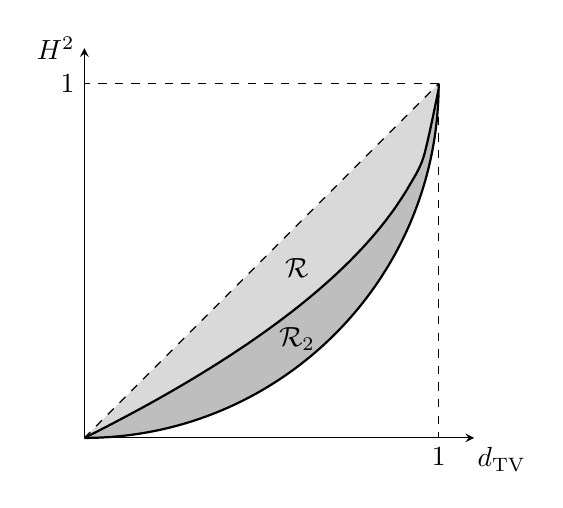
\begin{tikzpicture}[scale=4.5]
	% Draw axes
	\draw[-stealth] (0, 0) -- (1.1, 0) node[below] {$\qquad d_{\mathrm{TV}}$};
	\draw[-stealth] (0, 0) -- (0, 1.1) node[left] {$H^2$};
	
	% Shade the region between the curves
	\begin{scope}
		\clip (0, 0) rectangle (1, 1); % Clip the area to the plot range
		\fill[gray, opacity=0.3] 
		(0,0) plot[domain=0:1, smooth, variable=\x] ({\x}, {1 - sqrt(1 - \x)}) -- (1,1) arc[start angle=0, end angle=-90, radius=1] -- cycle;
	\end{scope}
    \begin{scope}
    	\clip (0, 0) rectangle (1, 1); % Clip to the plot area
    	\fill[gray, opacity=0.3] 
    	(0,0) arc[start angle=-90, end angle=0, radius=1] --
    	plot[domain=1:0, smooth, variable=\x] ({\x}, {\x}) -- cycle;
    \end{scope}
	
	% Plot y = 1 - sqrt(1 - x)
	\draw[domain=0:1, smooth, variable=\x, black, thick] 
	plot ({\x}, {1 - sqrt(1 - \x)});
	
	% Plot y = 1 - sqrt(1 - x^2)
	\draw[thick] (0,0) arc[start angle=-90, end angle=0, radius=1];
	
	% Add dashed lines at x=1 and y=1
	\draw[dashed] (1, 1) -- (1, 0) node[below] {$1$};
	\draw[dashed] (0, 0) -- (1, 1);
	\draw[dashed] (1, 1) -- (0, 1) node[left] {$1$};
	
	\node at (0.6, 0.48) {$\cal{R}$};
	\node at (0.6, 0.28) {$\cal{R}_2$};
\end{tikzpicture}
\end{center}
The sandwich bound is described by the diagonal line and the lower arc. According to our discussion, this sandwich bound is non-improvable. Under the constraint $d_{\mathrm{TV}}(P,Q)=t$, the upper bound is attained when $$P=\mathrm{Bernoulli}\left(\frac{1-t}{2}\right),Q=\mathrm{Bernoulli}\left(\frac{1+t}{2}\right),$$ and the lower bound is attained when $$P=(1-t,t,0),Q=(1-t,0,t).$$
\begin{theorem}[Total variation versus chi-square divergence]
Let $P$ and $Q$ be two probability measure on some measurable space. Then
\begin{align*}
	\chi^2(P\Vert Q)\geq f(d_\mathrm{TV}(P,Q)),\quad where\ \ f(t)=\begin{cases}
		4t^2, &0\leq t\leq\frac{1}{2},\\
		\frac{t}{1-t}, &\frac{1}{2}<t\leq 1.
	\end{cases}
\end{align*}
\end{theorem}
\begin{proof}
We consider the distributions $P=\mathrm{Bernoulli}(p)$ and $Q=\mathrm{Bernoulli}(q)$, where $0\leq p,q\leq 1$. Clearly,
\begin{align*}
	d_\mathrm{TV}(P,Q)=\vert q-p\vert,\quad \chi^2(P\Vert Q)=\frac{p^2}{q}+\frac{(1-p)^2}{1-q}-1=\frac{(q-p)^2}{q(1-q)}.
\end{align*} 
The joint range of $d_{\mathrm{TV}}$ and $H^2$ is
\begin{align*}
	\cal{R}_2=\left\{\left(\vert q-p\vert,\frac{(q-p)^2}{q(1-q)}\right):0\leq p,q\leq 1\right\}
\end{align*}
We fix $d_\mathrm{TV}(P,Q)=\vert q-p\vert =t\in(0,1)$. It turns out that
\begin{align*}
	\chi^2(P\Vert Q)=\frac{t^2}{q(1-q)}=\frac{t^2}{q(1-q)}.
\end{align*}
\begin{itemize}
\item If $t\leq\frac{1}{2}$, the minimum is attained when $q=\frac{1}{2}$ and $p=\frac{1}{2}-t$, and $\chi^2(P\Vert Q)=4t^2$; 
\item If $t>\frac{1}{2}$, the minimum is attained when $q=t$ and $p=0$, and $\chi^2(P\Vert Q)=\frac{t}{1-t}$. 
\end{itemize}
We consider the function $f:[0,1]\to\bbR_+$ defined as follows:
\begin{align*}
	f(t)=\begin{cases}
		4t^2, &0\leq t\leq\frac{1}{2},\\
		\frac{t}{1-t}, &\frac{1}{2}<t\leq 1.
	\end{cases}
\end{align*}
Then $f$ is a convex function on $[0,1]$, and $\cal{R}_2$ is the epigraph $\left\{(t,x):0\leq t\leq 1,\ x\geq f(t)\right\}$. Since $\cal{R}_2$ is convex, we have $\cal{R}=\conv(\cal{R}_2)=\cal{R}_2$. The desired bound follows this range.
\end{proof}
\paragraph{Remark.} We visualize the joint range of $d_{\mathrm{TV}}$ and $\chi^2$ in the following figure.
\begin{center}
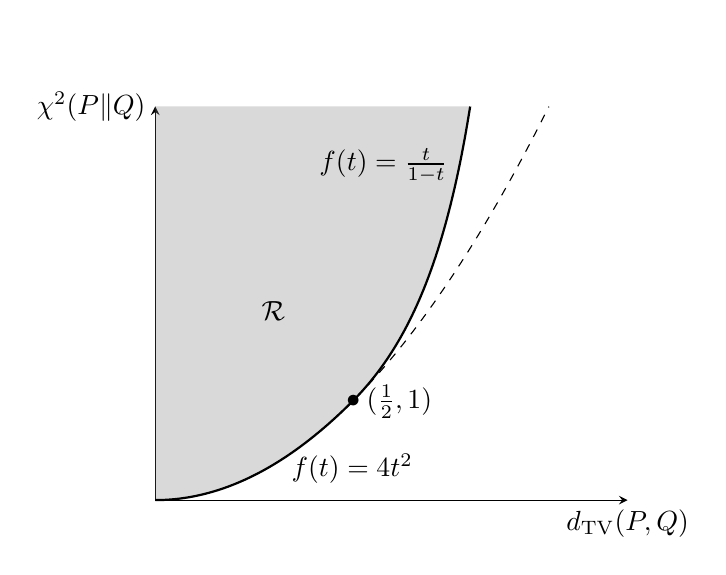
\begin{tikzpicture}[scale=5]
	% Draw axes
	\draw[-stealth] (0, 0) -- (1.2, 0) node[below] {$d_\mathrm{TV}(P,Q)$};
	\draw[-stealth] (0, 0) -- (0, 1) node[left] {$\chi^2(P\Vert Q)$};
	
	% Shade the region above the curve
	\begin{scope}
		\clip (0, 0) rectangle (1, 1.2); % Clip to the plot area
		\fill[gray, opacity=0.3] 
		plot[domain=0:0.5, smooth, variable=\x] ({\x}, {\x*\x}) --
		plot[domain=0.5:0.8, smooth, variable=\x] ({\x}, {0.25*\x/(1-\x)}) --
		(0.8, 1) -- (0, 1) -- cycle;
	\end{scope}
	
	% Plot f(t) = 4t^2 on [0, 1/2]
	\draw[domain=0:0.5, smooth, variable=\x, black, thick] 
	plot ({\x}, {\x*\x});
	\draw[domain=0:1, smooth, variable=\x, black, dashed] 
	plot ({\x}, {\x*\x});
	
	% Plot f(t) = t/(1-t) on [1/2, 1]
	\draw[domain=0.5:0.8, smooth, variable=\x, black, thick] 
	plot ({\x}, {0.25*\x/(1-\x)});
	\node at (0.3, 0.48) {$\cal{R}$};
	\node at (0.503, 0.25) {$\bullet$};
	\node at (0.62, 0.25) {$(\frac{1}{2},1)$};
	\node at (0.50, 0.08) {$f(t)=4t^2$};
	\node at (0.58, 0.85) {$f(t)=\frac{t}{1-t}$};
\end{tikzpicture}
\end{center}
A direct corollary of this range is that as $d_\mathrm{TV}(P,Q)\to 1$, we have $\chi^2(P\Vert Q)\to\infty$.

\begin{theorem}[Total variation versus Le Cam divergence]
	Let $P$ and $Q$ be two probability measure on some measurable space. Then
	\begin{align*}
		d_\mathrm{TV}(P,Q)^2\leq\mathrm{Le}(P\Vert Q)\leq d_\mathrm{TV}(P,Q).
	\end{align*}
\end{theorem}
\begin{proof}
	We consider the distributions $P=\mathrm{Bernoulli}(p)$ and $Q=\mathrm{Bernoulli}(q)$, where $0\leq p,q\leq 1$. Clearly,
	\begin{align*}
		d_\mathrm{TV}(P,Q)=\vert q-p\vert,\quad \Le(P,Q)=\frac{(p-q)^2}{2(p+q)}+\frac{(p-q)^2}{2(2-p-q)}.
	\end{align*} 
	The joint range of $d_{\mathrm{TV}}$ and $H^2$ is
	\begin{align*}
		\cal{R}_2=\left\{\left(\vert q-p\vert,\frac{(p-q)^2}{2(p+q)}+\frac{(p-q)^2}{2(2-p-q)}\right):0\leq p,q\leq 1\right\}
	\end{align*}
	We fix $d_\mathrm{TV}(P,Q)=\vert q-p\vert =t\in(0,1)$. It turns out that
	\begin{align*}
		\Le(P, Q)=\frac{t^2}{(2p+t)(2-2p-t)}.
	\end{align*}
	Over the interval $0\leq p\leq 1-t$, we have
	\begin{align*}
		t^2\leq\Le(P, Q)\leq\frac{t}{2-t}.
	\end{align*}
	Therefore, the joint range is
	\begin{align*}
		\cal{R}_2=\left\{(t,x):0\leq t\leq 1,\ t^2\leq x\leq\frac{t}{2-t}\right\},\quad\cal{R}=\conv(\cal{R}_2)=\left\{(t,x):0\leq t\leq 1,\ t^2\leq x\leq t\right\}.
	\end{align*}
	The desired inequality follows from this joint range.
\end{proof}
\paragraph{Remark.} We visualize the joint range of $d_\mathrm{TV}(P,Q)$ and $\Le(P,Q)$ in the following figure.
\begin{center}
	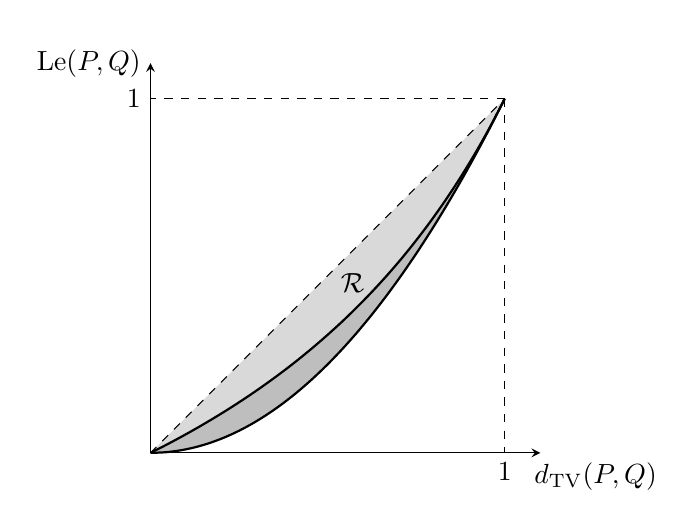
\begin{tikzpicture}[scale=4.5]
		% Draw axes
		\draw[-stealth] (0, 0) -- (1.1, 0) node[below] {$\qquad\qquad d_\mathrm{TV}(P,Q)$};
		\draw[-stealth] (0, 0) -- (0, 1.1) node[left] {$\Le(P, Q)$};
		
		% Shade the region above the curve
		\begin{scope}
			\clip (0, 0) rectangle (1, 1.2); % Clip to the plot area
			\fill[gray, opacity=0.3] 
			plot[domain=0:1, smooth, variable=\x] ({\x}, {\x*\x}) --
			plot[domain=1:0, smooth, variable=\x] ({\x}, {\x/(2-\x)}) -- cycle;
		\end{scope}
		\begin{scope}
			\clip (0, 0) rectangle (1, 1.2); % Clip to the plot area
			\fill[gray, opacity=0.3] 
			plot[domain=0:1, smooth, variable=\x] ({\x}, {\x*\x}) --
			plot[domain=1:0, smooth, variable=\x] ({\x}, {\x}) -- cycle;
		\end{scope}
		
		% Plot f(t) = 4t^2 on [0, 1/2]
		\draw[domain=0:1, smooth, variable=\x, black, thick] 
		plot ({\x}, {\x*\x});
		\draw[domain=0:1, smooth, variable=\x, black, thick] 
		plot ({\x}, {\x/(2-\x)});
		
		\node at (0.57, 0.48) {$\cal{R}$};
		% Add dashed lines at x=1 and y=1
		\draw[dashed] (1, 1) -- (1, 0) node[below] {$1$};
		\draw[dashed] (0, 0) -- (1, 1);
		\draw[dashed] (1, 1) -- (0, 1) node[left] {$1$};
	\end{tikzpicture}
\end{center}

\begin{example}[Total variation versus Jensen-Shannon divergence]
	Let $P$ and $Q$ be two probability measure on some measurable space. Then
	\begin{align*}
		\frac{1-d_\mathrm{TV}(P,Q)}{2}\log\left(1-d_\mathrm{TV}(P,Q)\right)+\frac{1+d_\mathrm{TV}(P,Q)}{2}\log(1+d_\mathrm{TV}(P,Q))\leq d_\mathrm{JS}(P\Vert Q)\leq \log 2\cdot d_\mathrm{TV}(P,Q).
	\end{align*}
\end{example}
\begin{proof}
	We consider the distributions $P=\mathrm{Bernoulli}(p)$ and $Q=\mathrm{Bernoulli}(q)$, where $0\leq p,q\leq 1$. Then
	\begin{align*}
		d_\mathrm{TV}(P,Q)=\vert q-p\vert,\quad d_\mathrm{JS}(P,Q)=H\left(\frac{p+q}{2}\right)-\frac{1}{2}H(p)-\frac{1}{2}H(q).
	\end{align*} 
	The joint range of $d_{\mathrm{TV}}$ and $d_\mathrm{JS}$ is
	\begin{align*}
		\cal{R}_2=\left\{\left(\vert q-p\vert,H\left(\frac{p+q}{2}\right)-\frac{1}{2}H(p)-\frac{1}{2}H(q)\right):0\leq p\leq q\leq 1\right\}
	\end{align*}
	We fix $p=\alpha-\frac{t}{2},q=\alpha+\frac{t}{2}$. It turns out that
	\begin{align*}
		d_\mathrm{JS}(P,Q)=H(\alpha)-\frac{1}{2}H\left(\alpha-\frac{t}{2}\right)-\frac{1}{2}H\left(\alpha+\frac{t}{2}\right).
	\end{align*}
	Over the interval $\frac{t}{2}\leq \alpha\leq 1-\frac{t}{2}$, we have
	\begin{align*}
		\frac{\partial}{\partial\alpha}d_\mathrm{JS}(P,Q)&=\log\frac{1-\alpha}{\alpha}-\frac{1}{2}\left(\log\frac{1-\alpha-\frac{t}{2}}{\alpha+\frac{t}{2}}+\log\frac{1-\alpha+\frac{t}{2}}{\alpha+\frac{t}{2}}\right),\\
		\frac{\partial^2}{\partial\alpha^2}d_\mathrm{JS}(P,Q)&=\frac{t^2}{\alpha(4\alpha^2-t^2)}+\frac{t^2}{4(1-\alpha)((1-\alpha)^2-t^2)}>0.
	\end{align*}
	Hence $d_\mathrm{JS}(P,Q)$ attains minimum when $\alpha=\frac{t}{2}$ or $1-\frac{t}{2}$, and attains maximum when $\alpha=\frac{1}{3}$.
	\begin{align*}
		H\left(\frac{t}{2}\right)-\frac{H(t)}{2}\leq d_\mathrm{JS}(P,Q)\leq H\left(\frac{1}{2}\right)-\frac{1}{2}H\left(\frac{1-t}{2}\right)-\frac{1}{2}H\left(\frac{1+t}{2}\right).
	\end{align*}
	Therefore
	\begin{align*}
		\cal{R}_2&=\left\{(t,x):\frac{1-t}{2}\log(1-t)+\frac{1+t}{2}\log(1+t)\leq x\leq H\left(\frac{t}{2}\right)-\frac{H(t)}{2}  \right\},\\
		\cal{R}&=\conv(\cal{R}_2)=\left\{(t,x):\frac{1-t}{2}\log(1-t)+\frac{1+t}{2}\log(1+t)\leq x\leq t\log 2 \right\}.
	\end{align*}
The desired bound follows from the joint range.
\end{proof}
\paragraph{Remark.} We visualize the joint range of $d_\mathrm{TV}(P,Q)$ and $d_\mathrm{JS}(P,Q)$ in the following figure.
\begin{center}\vspace{-1.3cm}
	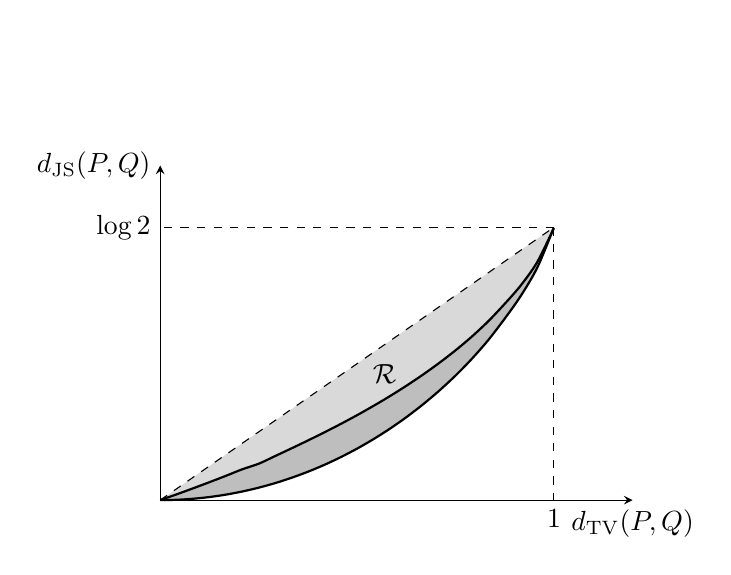
\begin{tikzpicture}[scale=5]
		% Draw axes
		\draw[-stealth] (0, 0) -- (1.2, 0) node[below] {$d_\mathrm{TV}(P,Q)$};
		\draw[-stealth] (0, 0) -- (0, 0.85) node[left] {$d_\mathrm{JS}(P, Q)$};
		% Shade the region above the curve
		\begin{scope}
			\clip (0, 0) rectangle (1, 1.2); % Clip to the plot area
			\fill[gray, opacity=0.3] 
			plot[domain=0.001:0.999, smooth, variable=\x] ({\x}, {-\x/2*ln(\x/2)-(1-\x/2)*ln(1-\x/2)+\x/2*ln(\x)+(1-\x)/2*ln(1-\x)}) --
			plot[domain=0.999:0, smooth, variable=\x] ({\x}, {0.5*(1-\x)*ln(1-\x)+0.5*(1+\x)*ln(1+\x)}) -- cycle;
		\end{scope}
		\begin{scope}
			\clip (0, 0) rectangle (1, 1.2); % Clip to the plot area
			\fill[gray, opacity=0.3] 
			plot[domain=0:1, smooth, variable=\x] ({\x}, {0.5*(1-\x)*ln(1-\x)+0.5*(1+\x)*ln(1+\x)}) --
			plot[domain=1:0, smooth, variable=\x] ({\x}, {ln(2)*\x}) -- cycle;
		\end{scope}
		
		% Plot f(t) = 4t^2 on [0, 1/2]
		\draw[domain=0.001:0.999, smooth, variable=\x, black, thick] 
		plot ({\x}, {-\x/2*ln(\x/2)-(1-\x/2)*ln(1-\x/2)+\x/2*ln(\x)+(1-\x)/2*ln(1-\x)});
		\draw[domain=0:1, smooth, variable=\x, black, thick] 
		plot ({\x}, {0.5*(1-\x)*ln(1-\x)+0.5*(1+\x)*ln(1+\x)});
		
		\node at (0.57, 0.32) {$\cal{R}$};
		% Add dashed lines at x=1 and y=1
		\draw[dashed] (1, 0.693) -- (0, 0.693) node[left] {$\log 2$};
		\draw[dashed] (0, 0) -- (1, 0.693);
		\draw[dashed] (1, 0.693) -- (1, 0) node[below] {$1$};
	\end{tikzpicture}
\end{center}

\begin{example}[Total variation versus Kullback-Leibler divergence]
The joint range between KL and TV is shown in the following figure. Although there is no known close-form expression, the following parametric formula of the lower boundary is known:
	\begin{align*}
		\begin{cases}
			\mathrm{TV}_t=\frac{t}{2}\left(1-\left(\coth(t)-\frac{1}{t}\right)^2\right)\\
			\mathrm{KL}_t=t\coth(t)+\log\left(t\,\mathrm{csch}(t)\right)-t^2\mathrm{csch}^2(t)
		\end{cases},\quad t\geq 0.
	\end{align*}
A direct corollary of this formula is Vajda's lower bound:
	\begin{align*}
		D(P\Vert Q)\geq\log\frac{1+d_\mathrm{TV}(P,Q)}{1-d_\mathrm{TV}(P,Q)}-\frac{2d_\mathrm{TV}(P,Q)}{1+d_\mathrm{TV}(P,Q)}.
	\end{align*}
\end{example}
\begin{center}
	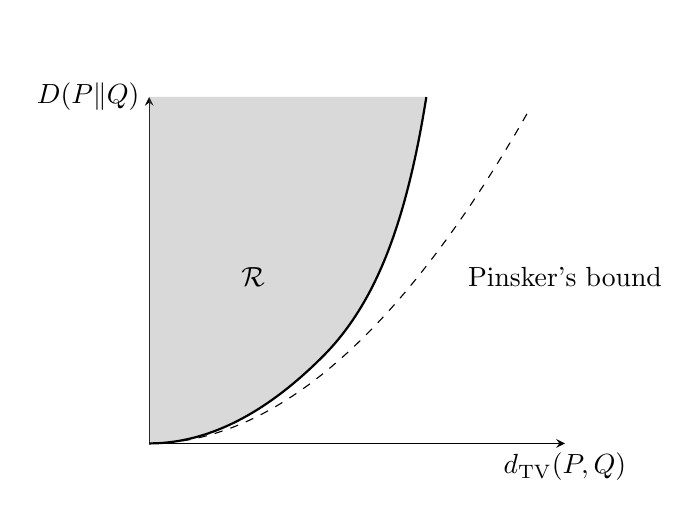
\begin{tikzpicture}[scale=4.4]
		% Draw axes
		\draw[-stealth] (0, 0) -- (1.2, 0) node[below] {$d_\mathrm{TV}(P,Q)$};
		\draw[-stealth] (0, 0) -- (0, 1) node[left] {$D(P\Vert Q)$};
		
		% Shade the region above the curve
		\begin{scope}
			\clip (0, 0) rectangle (1, 1.2); % Clip to the plot area
			\fill[gray, opacity=0.3] 
			plot[domain=0:0.5, smooth, variable=\x] ({\x}, {\x*\x}) --
			plot[domain=0.5:0.8, smooth, variable=\x] ({\x}, {0.25*\x/(1-\x)}) --
			(0.8, 1) -- (0, 1) -- cycle;
		\end{scope}
		
		% Plot f(t) = 4t^2 on [0, 1/2]
		\draw[domain=0:0.5, smooth, variable=\x, black, thick] 
		plot ({\x}, {\x*\x});
		\draw[domain=0:1.1, smooth, variable=\x, black, dashed] 
		plot ({\x}, {0.8*\x*\x});
		
		% Plot f(t) = t/(1-t) on [1/2, 1]
		\draw[domain=0.5:0.8, smooth, variable=\x, black, thick] 
		plot ({\x}, {0.25*\x/(1-\x)});
		\node at (0.3, 0.48) {$\cal{R}$};
		\node at (1.2, 0.48) {Pinsker's\ bound};
	\end{tikzpicture}
\end{center}

\newpage
\subsection{Pearson $\chi^2$-Divergence and Information Bounds}
The Pearson $\chi^2$-divergence is special because most $f$-divergences are locally $\chi^2$-like. 
\begin{theorem}
Let $D_f$ be an $f$-divergence such that $f\in C^2(\bbR_+)$ and $\limsup_{x\to\infty}f^{\prime\prime}(x)<\infty$. Then
\begin{itemize}
\item[(i)] If $\chi^2(Q\Vert P)<\infty$, then for any $0<\lambda<1$,
\begin{align*}
	D_f(\lambda Q+(1-\lambda)P\Vert P)<\infty;
\end{align*}
\item[(ii)] If $\chi^2(Q\Vert P)<\infty$,
\begin{align}
	\lim_{\lambda\to 0^+}\frac{1}{\lambda^2}D_f(\lambda Q+(1-\lambda)P\Vert P)=\frac{f^{\prime\prime}(1)}{2}\chi^2(Q\Vert P).\label{localchisq}
\end{align}
\end{itemize}
\end{theorem}
\begin{proof}
We will use the integral remainder of Taylor's expansion:
\begin{align*}
	f(x)&=f(a)+f^\prime(a)(x-a)+(x-a)^2\int_0^1(1-\theta)f^{\prime\prime}(a+\theta(x-a))\,d\theta.
\end{align*}
For any $0<\lambda<1$,
\begin{align*}
	&D_f(\lambda Q+(1-\lambda)P\Vert P)=\int f\left(1+\lambda\frac{dQ-dP}{dP}\right)dP\\
	&\quad=\int\left(f(1)+f^\prime(1)\left(\lambda\frac{dQ-dP}{dP}\right)+\left(\lambda\frac{dQ-dP}{dP}\right)^2\int_0^1(1-\theta)f^{\prime\prime}\left(1+\theta\lambda\frac{dQ-dP}{dP}\right)d\theta\right)dP\\
	&\quad=\lambda^2\int\left(\frac{dQ}{dP}-1\right)^2\left(\int_0^1(1-\theta)f^{\prime\prime}\left(1+\theta\lambda\frac{dQ-dP}{dP}\right)d\theta\right)\,dP.
\end{align*}
Since $1+\theta\lambda\frac{dQ-dP}{dP}\geq 1-\lambda$ and $\limsup_{x\to\infty}f^{\prime\prime}(x)<\infty$, the function $f^{\prime\prime}$ is bounded on $[1-\lambda,\infty)$. Hence
\begin{align}
	\int_0^1(1-\theta)f^{\prime\prime}\left(1+\theta\lambda\frac{dQ-dP}{dP}\right)d\theta\leq\frac{1}{2}\sup_{x\in[1-\lambda,\infty)}f^{\prime\prime}(x):=C_\lambda,\label{chisqbound1}
\end{align}
and therefore $D_f(\lambda Q+(1-\lambda)P\Vert P)\leq\lambda^2C_\lambda\chi^2(Q\Vert P)<\infty$. To prove (ii), it remains to determine
\begin{align*}
	\lim_{\lambda\to 0^+}\frac{1}{\lambda^2}D_f(\lambda Q+(1-\lambda)P\Vert P)=\lim_{\lambda\to 0^+}\int\left(\frac{dQ}{dP}-1\right)^2\left(\int_0^1(1-\theta)f^{\prime\prime}\left(1+\theta\lambda\frac{dQ-dP}{dP}\right)d\theta\right)\,dP.
\end{align*}
According to the bound (\ref{chisqbound1}), for all $0<\lambda<\frac{1}{2}$,
\begin{align*}
	\left(\frac{dQ}{dP}-1\right)^2\int_0^1(1-\theta)f^{\prime\prime}\left(1+\theta\lambda\frac{dQ-dP}{dP}\right)d\theta\leq C_{\frac{1}{2}}\left(\frac{dQ}{dP}-1\right)^2\in L^1(\cal{X},\mathscr{F},P).
\end{align*}
By dominated convergence theorem,
\begin{align}
	&\lim_{\lambda\to 0^+}\int\left(\frac{dQ}{dP}-1\right)^2\left(\int_0^1(1-\theta)f^{\prime\prime}\left(1+\theta\lambda\frac{dQ-dP}{dP}\right)d\theta\right)\,dP\notag\\
	&\quad =\int\left(\frac{dQ}{dP}-1\right)^2\left(\lim_{\lambda\to 0^+}\int_0^1(1-\theta)f^{\prime\prime}\left(1+\theta\lambda\frac{dQ-dP}{dP}\right)d\theta\right)\,dP\label{chisqdominate}\\
	&\quad =\int\left(\frac{dQ}{dP}-1\right)^2\frac{f^{\prime\prime}(1)}{2}\,dP=\frac{f^{\prime\prime}(1)}{2}\chi^2(Q\Vert P)\notag.
\end{align}
Thus we complete the proof.
\end{proof}
\paragraph{Remark.} In fact, the identity (\ref{localchisq}) remains correct even if $\chi^2(Q\Vert P)=\infty$ and $f^{\prime\prime}(1)>0$, i.e. $$D_f(\lambda Q+(1-\lambda)P\Vert P)=\omega(\lambda^2),\quad\lambda\to 0.$$ To see this, under the condition $Q\ll P$, we replace the equality (\ref{chisqdominate}) with ``$\geq$'' by Fatou's lemma:
\begin{align}
\lim_{\lambda\to 0^+}\int\left(\frac{dQ}{dP}-1\right)^2\left(\int_0^1(1-\theta)f^{\prime\prime}\left(1+\theta\lambda\frac{dQ-dP}{dP}\right)d\theta\right)\,dP
\geq\frac{f^{\prime\prime}(1)}{2}\chi^2(Q\Vert P).
\end{align}
Since $\chi^2(Q\Vert P)=\infty$ and $f^{\prime\prime}(1)>0$, the RHS of the last display is $\infty$, and the equality holds naturally.

\paragraph{Parameter estimation.} Let $\{P_\theta,\theta\in\Theta\}$ be a family of probability distributions parameterized by $\theta\in\Theta$. The estimation of parameter $\theta$ can be described by the following Markov chain:
\begin{align*}
	\theta^*\to X\to\wh{\theta},
\end{align*}
where $\theta^*$ is the true parameter, the sample $X\sim P_{\theta^*}$ is drawn from the distribution $P_{\theta^*}$, and  the estimator $\wh{\theta}=\wh{\theta}(X)$ is a (possibly random) mapping from the sample space $\cal{X}$ to the parameter space $\Theta$. We use the \textit{quadratic loss} to evaluate the difference between the real and the predicted parameter, i.e. $\ell(\wh{\theta})=\vert\wh{\theta}-\theta^*\vert^2$. The \textit{mean-squared error/risk} of estimator $\wh{\theta}$ when the real parameter is given by $\theta^*$ is
\begin{align*}
	R_{\theta^*}(\wh{\theta})=\E_{\theta^*}[\vert\wh{\theta}-\theta^*\vert^2]=\E_{X\sim P_{\theta^*}}\left[\bigl\vert\wh{\theta}(X)-\theta^*\bigr\vert^2\right].
\end{align*}
For an estimator $\wh{\theta}$ of $\theta$, we have the following Hammersley-Chapman-Robbins (HCR) lower bound of risk.

\begin{theorem}[Univariate Hammersley-Chapman-Robbins bound]
If $\Theta\subset\bbR$, any estimator $\wh\theta$ satisfies
\begin{align*}
\var_{\theta^*}(\wh{\theta})\geq\sup_{\theta\in\Theta:\theta\neq\theta^*}\frac{\bigl(\E_{\theta^*}[\wh{\theta}]-\E_{\theta}[\wh{\theta}]\bigr)^2}{\chi^2(P_\theta\Vert P_{\theta^*})},\quad\forall\theta^*\in\Theta.
\end{align*}
\end{theorem}
\begin{proof}
For all $\theta\in\Theta$, the distribution $P_\theta$ of $X$ and the mapping rule $\wh\theta=\wh\theta(X)$ together induce a distribution $Q_\theta$ of the estimator $\wh{\theta}$. We fix $\theta^*,\theta\in\Theta$ with $\theta\neq\theta^*$. By data processing inequality,
\begin{align}
	\chi^2(P_\theta\Vert P_{\theta^*})\geq\chi^2(Q_\theta\Vert Q_{\theta^*}).\label{chisqdatapro}
\end{align}
We take $h(x)=x$ in the variational representation (\ref{chisqdivvarrep}) of $\chi^2$-divergence, hence
\begin{align}
	\chi^2(Q_\theta\Vert Q_{\theta^*})\geq\frac{\bigl(\E_{\theta^*}[\wh{\theta}]-\E_{\theta}[\wh{\theta}]\bigr)^2}{\var_{\theta^*}(\wh{\theta})}.\label{chisqvarlin}
\end{align}
Combining (\ref{chisqdatapro}) and (\ref{chisqvarlin}), we get
\begin{align*}
	\var_{\theta^*}(\wh{\theta})\geq\frac{\bigl(\E_{\theta^*}[\wh{\theta}]-\E_{\theta}[\wh{\theta}]\bigr)^2}{\chi^2(P_\theta\Vert P_{\theta^*})}.
\end{align*}
Since this inequality holds for all $\theta\neq\theta^*$, we take supremum on both sides to get the desired bound.
\end{proof}
\paragraph{Remark.} Define the \textit{bias function} of $\wh\theta$ by $b(\theta)=\E_\theta[\wh{\theta}]-\theta$. According to the bias-variance decomposition,
\begin{align*}
	R_{\theta^*}(\wh{\theta})=\E_{\theta^*}[(\wh{\theta}-\theta^*)^2]\geq\sup_{\theta\in\Theta:\theta\neq\theta^*}\frac{\bigl(\E_{\theta^*}[\wh{\theta}]-\E_{\theta}[\wh{\theta}]\bigr)^2}{\chi^2(P_\theta\Vert P_{\theta^*})}+b(\theta^*)^2.
\end{align*}

\begin{theorem}[Multivariate Hammersley-Chapman-Robbins bound]
If $\Theta\subset\bbR^n$, any estimator $\wh\theta$ satisfies
	\begin{align*}
		\chi^2(P_\theta\Vert P_{\theta^*})\geq\bigl(\E_{\theta^*}[\wh{\theta}]-\E_{\theta}[\wh{\theta}]\bigr)^\top\cov_{\theta^*}(\wh{\theta})^{-1}\bigl(\E_{\theta^*}[\wh{\theta}]-\E_{\theta}[\wh{\theta}]\bigr),\quad\forall\theta^*,\theta\in\Theta.
	\end{align*}
\end{theorem}
\begin{proof}
Based on the same procedure establishing (\ref{chisqdatapro}), we take $h(x)=\xi^\top x$ in the variational representation (\ref{chisqdivvarrep}) of $\chi^2$-divergence, where $\xi\in\bbR^n\backslash\{0\}$. Then
\begin{align}
	\chi^2(Q_\theta\Vert Q_{\theta^*})\geq\frac{\bigl(\xi^\top\E_{\theta^*}[\wh{\theta}]-\xi^\top\E_{\theta}[\wh{\theta}]\bigr)^2}{\xi^\top\cov_{\theta^*}(\wh{\theta})\xi}.\label{chisqvarmullin}
\end{align}
Combining (\ref{chisqdatapro}), (\ref{chisqvarlin}) and taking the supremum with respect to $\xi\in\bbR^n\backslash\{0\}$, we get
	\begin{align*}
		\chi^2(P_\theta\Vert P_{\theta^*})\geq\sup_{\xi\in\bbR^n\backslash\{0\}}\frac{\xi^\top\bigl(\E_{\theta^*}[\wh{\theta}]-\E_{\theta}[\wh{\theta}]\bigr)\bigl(\E_{\theta^*}[\wh{\theta}]-\E_{\theta}[\wh{\theta}]\bigr)^\top\xi}{\xi^\top\cov_{\theta^*}(\wh{\theta})\xi}.
	\end{align*}
Using the fact $\sup_{\xi\in\bbR^n\backslash\{0\}}\frac{\langle w,\xi\rangle^2}{\xi^\top M\xi}=w^\top M^{-1}w$ from linear algebra, we obtain the desired bound. 
\end{proof}

\paragraph{Score function.} In many cases, we can express $P_\theta$ in form of the likelihood function:
\begin{align*}
	\bbP_\theta(X\in A)=\int_A P_\theta(x)\,\mu(dx),\quad A\in\mathscr{F},
\end{align*}
where $\mu$ is a dominating measure. For example, $\mu$ is the counting measure in the discrete case or the Lebesgue measure in the continuous case. The partial derivative of the log-likelihood $\log P_\theta(x)$ with respect to $\theta\in\Theta$ is called the \textit{score}. Under regularity conditions on $P_\theta(x)$\footnote{
To be specific, we assume $\Theta$ is an open subset of $\bbR^n$, and assume $\theta\mapsto P_\theta(x)$ to be a continuously differentiable function. For fixed parameter value $\theta_0\in\Theta$ and $\epsilon>0$, we consider the following conditions:
\begin{itemize}
\item[(i)] $\displaystyle\int_\cal{X} P_\theta(x)\,dx<\infty$ for all $\theta\in B(\theta_0,\epsilon):=\{\theta\in\Theta:\vert\theta-\theta^*\vert<\epsilon\}$;\vspace{0.07cm}
\item[(ii)] $\displaystyle\int_\cal{X}\frac{\partial}{\partial\theta}P_\theta(x)\,dx$ is continuous at $\theta=\theta_0$;\vspace{0.07cm}
\item[(ii')] $\displaystyle\int_\cal{X}\sup_{\theta\in B(\theta_0,\epsilon)}\left\vert\frac{\partial}{\partial\theta}P_\theta(x)\right\vert dx<\infty$;\vspace{0.07cm}
\item[(iii)] $\displaystyle\int_\cal{X}\int_{0}^{\epsilon}\left\vert\frac{\partial}{\partial\theta}P_{\theta_0+tu}(x)\right\vert dt\,dx<\infty$ for all unit vectors $\vert u\vert =1$.\vspace{0.07cm}
\end{itemize}
Under conditions (i), (ii) and (iii), we use Fubini's theorem:
\begin{align*}
	\frac{1}{h}\int_{\cal{X}}\left(P_{\theta_0+hu}(x)-P_{\theta_0}(x)\right)dx=\frac{1}{h}\int_\cal{X}\int_{0}^{h}u^\top\frac{\partial}{\partial\theta} P_{\theta_0+tu}(x)\, dt\,dx=\frac{1}{h}u^\top\int_{0}^{h}\int_\cal{X}\frac{\partial}{\partial\theta}P_\theta(x)\,dx\, dt,\quad\forall\vert u\vert=1.
\end{align*}
Letting $h\to 0$ on the both sides, we obtain
\begin{align*}
	\nabla_\theta\int_\cal{X}P_\theta(x)\,dx\,\bigg|_{\theta=\theta_0}=\int_\cal{X}\frac{\partial}{\partial\theta}P_{\theta_0}(x)\,dx
\end{align*}
Under conditions (i) and (ii'), for all $\vert h\vert<\epsilon$ and $\vert u\vert=1$, the difference quotients are dominated by an integrable function:
\begin{align*}
	\left\vert\frac{P_{\theta_0+hu}(x)-P_{\theta_0}(x)}{h}\right\vert=\left\vert\frac{1}{h}\int_{0}^{h}\frac{\partial}{\partial\theta}P_{\theta_0+tu}(x)d\theta\right\vert\leq\sup_{\theta\in B(\theta_0,\epsilon)}\left\vert\frac{\partial}{\partial\theta}P_\theta(x)\right\vert.
\end{align*}
By Dominated Convergence Theorem,
\begin{align*}
	\lim_{h\to 0}\int_{\cal{X}}\frac{P_{\theta_0+hu}(x)-P_{\theta_0}(x)}{h}\,dx=\int_{\cal{X}}\lim_{h\to 0}\frac{P_{\theta_0+hu}(x)-P_{\theta_0}(x)}{h}\,dx,\ \forall\vert u\vert=1\quad\Leftrightarrow\quad
	\nabla_\theta\int_\cal{X}P_\theta(x)\,dx\,\bigg|_{\theta=\theta_0}=\int_\cal{X}\frac{\partial}{\partial\theta}P_{\theta_0}(x)\,dx.
\end{align*}

}, the expectation of the score function evaluated at the true parameter $\theta$ is zero:
\begin{align*}
	\E_\theta\left[\frac{\partial}{\partial\theta}\log P_\theta(x)\right]=\int_\cal{X}\frac{\frac{\partial}{\partial\theta}P_\theta(x)}{P_\theta(x)}P_\theta(x)\,dx=\int_\cal{X}\frac{\partial}{\partial\theta}P_\theta(x)\,dx=\nabla_\theta\int_\cal{X}P_\theta(x)\,dx=0.
\end{align*}
\textbf{Fisher information.}\quad The \textit{Fisher information} $\cal{I}(\theta)$ is defined to be the covariance of the score when the true parameter is $\theta$:
\begin{align*}
	\mathcal{I}(\theta)=\E_\theta\left[\left(\frac{\partial}{\partial\theta}\log P_\theta(X)\right)\left(\frac{\partial}{\partial\theta}\log P_\theta(X)\right)^\top\right]=\int\frac{1}{P_\theta}\frac{\partial P_\theta}{\partial\theta}\frac{\partial P_\theta}{\partial\theta^\top}.
\end{align*}
Using the Taylor's expansion of $P_\theta$ at $\theta^*$, we have
\begin{align*}
	P_\theta-P_{\theta^*}=(\theta-\theta^*)^\top\frac{\partial P_{\theta^*}}{\partial\theta}+o(\vert\theta-\theta^*\vert).
\end{align*}
Under regularity conditions \footnote{
Define the remainder of the first-order Taylor expansion as follows:
\begin{align*}
	r_\theta=P_\theta-P_{\theta^*}-(\theta-\theta^*)^\top\frac{\partial P_{\theta^*}}{\partial\theta}=o(\vert\theta-\theta^*\vert).
\end{align*}
By Cauchy-Schwarz inequality, (\ref{fisherlocalchisq}) is valid if $r_\theta$ vanishes under the weighted inner product:
\begin{align*}
\int\frac{r_\theta^2(x)}{P_{\theta^*}(x)}\,dx=o(\vert\theta-\theta^*\vert^2).
\end{align*}
By Dominated Convergence Theorem, if the mapping $x\mapsto \frac{r_\theta^2(x)}{P_{\theta^*}(x)\vert\theta-\theta^*\vert^2}$ is dominated by some $L^1$-function on $\cal{X}$ within some deleted neighborhood $0<\vert\theta-\theta^*\vert<\epsilon$, we have
\begin{align*}
	\lim_{\theta\to\theta^*}\frac{1}{\vert\theta-\theta^*\vert^2}\int\frac{r_\theta^2(x)}{P_{\theta^*}(x)}\,dx=\int\lim_{\theta\to\theta^*}\frac{r_\theta^2(x)}{P_{\theta^*}(x)\vert\theta-\theta^*\vert^2}\,dx=0.
\end{align*} 
We can require that for some $\epsilon>0$,
\begin{align*}
	\int\sup_{\theta:0<\vert\theta-\theta^*\vert<\epsilon}\frac{r_\theta^2(x)}{P_{\theta^*}(x)\vert\theta-\theta^*\vert^2}\,dx<\infty.
\end{align*}}
on $P_\theta(x)$, 
\begin{align}
	\chi^2(P_\theta\Vert P_{\theta^*})&=\int\frac{(P_\theta-P_{\theta^*})^2}{P_{\theta^*}}\notag\\
	&=(\theta-\theta^*)^\top\cal{I}(\theta^*)(\theta-\theta^*)+o\left(\vert\theta-\theta^*\vert^2\right).\label{fisherlocalchisq}
\end{align}
Therefore, the $\chi^2$-divergence is ``locally Fisher information''. Using this property, we can derive a universal bound for estimation error in terms of Fisher information.

\begin{theorem}[Cramér-Rao bound]
Let $\Theta\subset\bbR$. Under regularity conditions, for the quadratic loss, any unbiased estimator $\wh\theta$ satisfies
\begin{align*}
	R_{\theta^*}(\wh{\theta})=\E_{\theta^*}[(\wh{\theta}-\theta^*)^2]\geq\frac{1}{\cal{I}(\theta^*)},\quad\forall\theta^*\in\Theta.
\end{align*}
where $\cal{I}(\theta^*)$ is the Fisher information evaluated at the true parameter $\theta^*\in\Theta$.
\end{theorem}
\begin{proof}
Using the Hammersley-Chapman-Robbins bound and the unbiasedness of $\wh\theta$,
\begin{align*}
	\E_{\theta^*}[(\wh{\theta}-\theta^*)^2]&\geq\lim_{\theta\to\theta^*}\frac{\bigl(\E_{\theta^*}[\wh{\theta}]-\E_{\theta}[\wh{\theta}]\bigr)^2}{\chi^2(P_\theta\Vert P_{\theta^*})}\\
	&=\lim_{\theta\to\theta^*}\frac{\bigl(\theta^*-\theta\bigr)^2}{(\theta^*-\theta)^2\cal{I}(\theta^*)+o\bigl((\theta^*-\theta)^2\bigr)}=\frac{1}{\cal{I}(\theta^*)}.
\end{align*}
Thus we complete the proof.
\end{proof}

For biased estimators, we also have a similar bound.

\newpage
\begin{theorem}[Biased Cramér-Rao bound]\label{biasedcramerrao}
Let $\Theta\subset\bbR$. Given an estimator $\wh\theta$, assume that the function $\theta\mapsto\E_\theta[\wh\theta]$ is continuously differentiable. Under regularity conditions, for the quadratic loss, the estimator $\wh\theta$ satisfies
	\begin{align*}
		R_{\theta^*}(\wh{\theta})=\E_{\theta^*}[(\wh{\theta}-\theta^*)^2]\geq\frac{(1+b^\prime(\theta^*))^2}{\cal{I}(\theta^*)}+b(\theta^*)^2,\quad\forall\theta^*\in\Theta,
	\end{align*}
	where $\cal{I}(\theta^*)$ is the Fisher information evaluated at  $\theta^*\in\Theta$, and $b(\theta)=\E_\theta[\wh{\theta}]-\theta$ is the bias of $\wh\theta$.
\end{theorem}
\begin{proof}
Using the Hammersley-Chapman-Robbins bound, we have
\begin{align*}
	\var_{\theta^*}(\wh{\theta})&\geq\lim_{\theta\to\theta^*}\frac{\bigl(\E_{\theta^*}[\wh{\theta}]-\E_{\theta}[\wh{\theta}]\bigr)^2}{\chi^2(P_\theta\Vert P_{\theta^*})}=\lim_{\theta\to\theta^*}\frac{\bigl(\theta-\theta^*+b(\theta)-b(\theta^*)\bigr)^2}{(\theta^*-\theta)^2\cal{I}(\theta^*)+o\bigl((\theta^*-\theta)^2\bigr)}=\frac{(1+b^\prime(\theta^*))^2}{\cal{I}(\theta^*)}.
\end{align*}
The result then follows from bias-variance decomposition.
\end{proof}

\begin{theorem}[General Cramér-Rao bound]\label{generalcramerrao}
Let $\Theta\subset\bbR^n$. Given an estimator $\wh\theta$, assume that the function $\theta\mapsto\E_\theta[\wh\theta]$ is continuously differentiable. Let $\phi(\theta)=\frac{\partial}{\partial\theta}\E_\theta[\wh\theta]$. Then estimator $\wh\theta$ satisfies
\begin{align*}
\cal{I}(\theta^*)\succeq\phi(\theta^*)\cov_{\theta^*}(\wh\theta)^{-1}\phi(\theta^*)^\top,\quad and\quad 
\cov_{\theta^*}\succeq\phi(\theta^*)(\wh\theta)\cal{I}(\theta^*)^{-1}\phi(\theta^*)^\top,
\end{align*}
where $A\succeq B$ denotes that $\xi^\top(A-B)\xi\geq 0$ for all $\xi\in\bbR^n$.
\end{theorem}
\begin{proof}
Fix any $\xi\in\bbR^n$. Since $\phi\mapsto\E_\theta[\wh{\theta}]$ is continuously differentiable, we have
\begin{align*}
\E_{\theta^*+h\xi}[\wh{\theta}]-\E_{\theta^*}[\wh{\theta}]=h\xi^\top\phi(\theta^*)+o(h).
\end{align*}
Plugging in this equation and (\ref{fisherlocalchisq}) into the multivariate Hammersley-Chapman-Robbins bound, we have
\begin{align*}
	\xi^\top\cal{I}(\theta^*)\xi+\frac{o(h^2)}{h^2}\geq \xi^\top\phi(\theta^*)\cov_{\theta^*}(\wh\theta)^{-1}\phi(\theta^*)^\top\xi+\frac{o(h^2)}{h^2}
\end{align*}
Letting $h\to 0$, we obtain the first bound. Furthermore, according to the univariate HCR bound,
\begin{align*}
	\xi^\top\cov_{\theta^*}(\wh{\theta})\xi=\var_{\theta^*}(\xi^\top\wh{\theta})\geq\frac{\bigl(\xi^\top\E_{\theta^*}[\wh{\theta}]-\xi^\top\E_{\theta}[\wh{\theta}]\bigr)^2}{\chi^2(P_\theta\Vert P_{\theta^*})}.
\end{align*}
For any $\eta\in\bbR^n$, letting $\theta=\theta^*+h\eta$, we have
\begin{align*}
	\xi^\top\cov_{\theta^*}(\wh{\theta})\xi\geq\frac{h^2\bigl(\xi^\top\phi(\theta^*)\eta\bigr)^2+o(h^2)}{h^2\eta^\top\cal{I}(\theta^*)\eta+o(h^2)}\to\frac{\bigl(\xi^\top\phi(\theta^*)\eta\bigr)^2}{\eta^\top\cal{I}(\theta^*)\eta},\quad\forall\eta\in\bbR^n.
\end{align*}
Using the fact $\sup_{\eta\in\bbR^n\backslash\{0\}}\frac{\langle w,\eta\rangle}{\eta^\top M\eta}=w^\top M^{-1}w$ from linear algebra, we have
\begin{align*}
	\xi^\top\cov_{\theta^*}(\wh{\theta})\xi\geq\xi^\top\phi(\theta^*)\cal{I}(\theta^*)^{-1}\phi(\theta^*)^\top\xi.
\end{align*}
Since $\xi\in\bbR^n$ is arbitrary, we obtain the second bound, concluding the proof.
\end{proof}
\paragraph{Remark.} If $\wh\theta$ is an unbiased estimator, $\phi(\theta)=\id_n$. We have the unbiased Cramér-Rao bound:
\begin{align*}
	\cov_{\theta^*}(\wh{\theta})\succeq\cal{I}(\theta^*)^{-1}.
\end{align*}
When the dimension $n=1$, the Theorem reduces to the case in Theorem \ref{biasedcramerrao}.

\paragraph{Bayesian case.} From a Bayesian perspective, in each experiment, the true parameter $\theta$ is subject to a prior distribution $\pi$ on $\Theta$.  The average risk of $\wh{\theta}$ over the prior $\pi$ is
\begin{align*}
	R_\pi(\wh{\theta})=\E_{\theta\sim\pi}R_\theta(\wh{\theta})=\E_{\theta\sim\pi}\left[(\wh\theta-\theta)^2\right].
\end{align*}
Given a prior distribution $\pi$, the Bayesian risk for $\pi$ is defined as the infimum of the average risk: 
\begin{align*}
	R_\pi^*=\inf_{\wh{\theta}}R_\pi(\wh\theta)=\inf_{\wh{\theta}}\E_{\theta\sim\pi}\left[(\wh\theta-\theta)^2\right]
\end{align*}

\begin{theorem}[Bayesian Cramér-Rao bound]
\begin{align*}
	R_\pi^*=\inf_{\wh{\theta}}R_\pi(\wh\theta)\geq\frac{1}{\E_{\theta\sim\pi}[\cal{I}(\theta)]+\cal{I}(\pi)},
\end{align*}
where $\cal{I}(\pi)=\int_{\Theta}\frac{\pi^\prime}{\pi}$ is the Fisher information of the prior.
\end{theorem}
\begin{proof}
Consider the following comparison of experiments:
\begin{align*}
p:\pi\to\theta\overset{X\sim p_{X|\theta}}{\xrightarrow{\hspace{1cm}}} X\to\wh{\theta},\qquad q:\wt\pi\to\theta\overset{X\sim q_{X|\theta}}{\xrightarrow{\hspace{1cm}}} X\to\wh{\theta}.
\end{align*}
By the data processing inequality and the variational representation,
\begin{align*}
	\chi^2(q_{\theta,X}\Vert p_{\theta,X})\geq\chi^2(q_{\theta,\wh\theta}\Vert p_{\theta,\wh\theta})\geq\chi^2(q_{\theta-\wh\theta}\Vert p_{\theta-\wh\theta})\geq\frac{\bigl(\E_p[\theta-\wh\theta]-\E_q[\theta-\wh\theta]\bigr)^2}{\var_p(\theta-\wh\theta)}
\end{align*}
Let $\wt\pi$ be the prior obtained by shifting $\pi$ by $\delta$, i.e. $\wt{\pi}(\theta)=\pi(\theta-\delta)$. We choose $p_{X|\theta}=P_\theta$ and $q_{X|\theta}=P_{\theta-\delta}$. Then $p_X=q_X$, and $p_{\wh\theta}=q_{\wh\theta}$. Hence $\E_q[\theta-\wh\theta]-\E_p[\theta-\wh\theta]=\delta$, and
\begin{align}
	\var_p(\theta-\wh\theta)\geq\frac{\delta^2}{\chi^2(q_{\theta,X}\Vert p_{\theta,X})}.\label{baysianhcr}
\end{align} 
On the other hand,
\begin{align*}
	&\chi^2(q_{\theta,X}\Vert p_{\theta,X})=\int\int\frac{(q_{\theta,X}-p_{\theta,X})^2}{p_{\theta,X}}\,dx\,d\theta=\int\int\frac{\left[q_\theta(q_{X|\theta}-p_{X|\theta})+(q_\theta-p_\theta)p_{X|\theta}\right]^2}{p_{\theta,X}}\,d\theta\,dx\\
	&\quad =\int\frac{q_\theta^2}{p_\theta}\,d\theta\int\frac{(q_{X|\theta}-p_{X|\theta})^2}{p_{X|\theta}}\,dx+\int\frac{(q_\theta-p_\theta)^2}{p_\theta}\,d\theta\int p_{X|\theta}\,dx+\int\frac{q_\theta(q_\theta-p_\theta)}{p_\theta}\,d\theta\int(q_{X|\theta}-p_{X|\theta})\,dx\\
	&\quad=\int\chi^2(q_{X|\theta}\Vert p_{X|\theta})\frac{q_\theta^2}{p_\theta}\,d\theta+\chi^2(q_\theta\Vert p_\theta).
\end{align*}
According to Taylor's expansion, we have $\chi^2(q_{X|\theta}\Vert p_{X|\theta})=\chi^2(P_{\theta-\delta}\Vert P_\theta)=\delta^2\cal{I}(\theta)+o(\delta^2)$, and $\chi^2(q_\theta\Vert p_\theta)=\chi^2(\pi(\cdot-\delta)\Vert \pi)=\delta^2\cal{I}(\pi)+o(\delta^2)$.
Hence
\begin{align}
	\chi^2(q_{\theta,X}\Vert p_{\theta,X})=\delta^2\E_{p_\theta}[\cal{I}(\theta)]+\delta^2\cal{I}(\pi)+o(\delta^2).\label{bayesianchisqdiv}
\end{align}
Combining (\ref{baysianhcr}) and (\ref{bayesianchisqdiv}), and letting $\delta\to 0$, we have
\begin{align*}
	\E[(\theta-\wh\theta)^2]\geq\var_{\theta\sim\pi}(\theta-\wh\theta)\geq\frac{1}{\E_{\theta\sim\pi}[\cal{I}(\theta)]+\cal{I}(\pi)}.
\end{align*}
Since $\wh{\theta}$ is arbitrary, we obtain the desired bound for Bayesian risk.
\end{proof}

\newpage
\subsection{Application: Kernel Density Estimator}
\paragraph{Setting.} In this section, we consider the estimation of the density of a channel output $Y$. Assume that we are given a known channel $P_{Y|X}$, and let $P_X$ be any unknown input distribution. Given observations $X_1,\cdots,X_n\overset{\text{i.i.d.}}{\sim}P_X$, the empirical distribution of $X$ is
\begin{align*}
	\wh{P}_n=\sum_{j=1}^n\delta_{X_j}.
\end{align*}
A natural estimate of the distribution of $Y$ is $P_{Y|X}\circ\wh{P}_n$. In many practical cases, the conditional density of $Y$ given $X=x$ is of the form $P_{Y|X=x}=\phi(\cdot -x)$, where $\phi$ is a fixed density. For example, the additional channel $Y=X+Z$ satisfies this formula when $Z\sim\phi$ is independent of $X$. In this case, we can think of $P_{Y|X}\circ\wh{P}_n$ as a \textit{kernel density estimator} (KDE), whose density is
\begin{align*}
	\wh{p}_n(y)=(\phi * \wh{P}_n)(y)=\frac{1}{n}\sum_{j=1}^n \phi(y-X_n).
\end{align*}
Using the fact that $\E[\wh{p}_n(y)]=p_Y(y)$ for all $y\in\bbR$, we have
\begin{align*}
	\E\left[D(P_{Y|X}\circ\wh{P}_n\Vert P_X)\right]&=\E\left[\int\wh{p}_n(y)\log\frac{\wh{p}_n(y)}{p_X(y)}\,dy\right]\\
	&=\E\left[\int\wh{p}_n(y)\log\frac{\wh{p}_n(y)}{p_Y(y)}\,dy\right]+\E\left[\int\wh{p}_n(y)\log\frac{p_Y(y)}{p_X(y)}\,dy\right]\\
	&=\E\left[\int\wh{p}_n(y)\log\frac{\wh{p}_n(y)}{p_Y(y)}\,dy\right]+\int\E\left[\wh{p}_n(y)\right]\log\frac{p_Y(y)}{p_X(y)}\,dy\\
	&=\E\left[D(P_{Y|X}\circ\wh{P}_n\Vert P_Y)\right]+D(P_Y\Vert P_X)
\end{align*}
In this section, we determine the convergence rate of the expected estimation error $\E[D(P_{Y|X}\circ\wh{P}_n\Vert P_Y)]$.
\paragraph{Mutual $\chi^2$-information.} Consider two random variables $X,Y\sim P_{X,Y}$. Let $P_X$ and $P_Y$ be the marginal distributions of $X$ and $Y$, respectively. The mutual information between $X$ and $Y$ is defined as
\begin{align*}
	I(X;Y)=D\left(P_{XY}\Vert P_XP_Y\right)=\int P_{XY}\log\frac{P_{XY}}{P_XP_Y}.
\end{align*}
Similarly, we define the mutual $\chi^2$-information between $X$ and $Y$ to be
\begin{align*}
	I_{\chi^2}(X;Y)=\chi^2\left(P_{XY}\Vert P_XP_Y\right).
\end{align*}
More generally, if $D_f$ is an $f$-divergence, the mutual $f$-information between $X$ and $Y$ is
\begin{align*}
	I_f(X;Y)=D_f\left(P_{XY}\Vert P_XP_Y\right).
\end{align*}
\begin{theorem}\label{kdeconvg}
Under the above setting, we have the following upper bound for the estimation error:
\begin{align*}
	\E\left[D(P_{Y|X}\circ\wh{P}_n\Vert P_Y)\right]\leq\log\left(1+\frac{1}{n}I_{\chi^2}(X;Y)\right);
\end{align*}
Moreover, we have the following lower bound for the estimation error:
\begin{align*}
	\lim_{n\to\infty} n\E\left[D(P_{Y|X}\circ\wh{P}_n\Vert P_Y)\right]\geq\frac{1}{2}I_{\chi^2}(X;Y).
\end{align*}
\end{theorem}
\begin{proof}
We first prove the upper bound. Note that
\begin{align*}
	\E\left[\chi^2(P_{Y|X}\circ\wh{P}_n\Vert P_Y)\right]&=\E\left[\int\frac{(\wh{p}_n(y)-p_Y(y))^2}{p_Y(y)}dy\right]\\
	&=\E\left[\int\frac{1}{p_Y(y)}\left(\frac{1}{n}\sum_{j=1}^n p_{Y|X}(y|X_j)-p_Y(y)\right)^2 dy\right]\\
	&=\int\frac{1}{p_Y(y)}\E\left[\left(\frac{1}{n}\sum_{j=1}^n p_{Y|X}(y|X_j)-p_Y(y)\right)^2\right]dy.
\end{align*}
For any $X_j\sim p_X$, we have
\begin{align*}
	\E\left[p_{Y|X}(y|X_j)-p_Y(y)\right]=0,
\end{align*}
and
\begin{align*}
	\int\frac{\E\left[(p_{Y|X}(y|X_j)-p_Y(y))^2\right]}{p_Y(y)}\,dy&=\int\int \frac{(p_{Y|X}(y|x)-p_Y(y))^2}{p_Y(y)}p_X(x)\,dx\,dy\\
	&=\int\int\frac{(p_{X,Y}(x,y)-p_X(x)p_Y(y))^2}{p_X(x)p_Y(y)}\,dx\,dy\\
	&=I_{\chi^2}(X;Y).
\end{align*}
Hence
\begin{align*}
	\E\left[\chi^2(P_{Y|X}\circ\wh{P}_n\Vert P_Y)\right]&=\frac{1}{n}I_{\chi^2}(X;Y).
\end{align*}
By (\ref{chisqklineq}) and Jensen's inequality,
\begin{align*}
	\E\left[D(P_{Y|X}\circ\wh{P}_n\Vert P_Y)\right]&\leq\E\left[\log\left(1+\chi^2(P_{Y|X}\circ\wh{P}_n\Vert P_Y)\right)\right]\\
	&\leq\log\left(1+\E\left[\chi^2(P_{Y|X}\circ\wh{P}_n\Vert P_Y)\right]\right)=\log\left(1+\frac{1}{n}I_{\chi^2}(X;Y)\right).
\end{align*}
To prove the lower bound, we let $X^*\sim\mathrm{Unif}(X_1,\cdots,X_n)$, and let $Y^*$ be the output of the channel $P_{Y|X}$ given the input $X^*$. Then $Y^*\overset{d}{=}Y$ marginally, and the joint distribution of $(X_{1:n},Y^*)$ is
\begin{align*}
	p^*(x_1,\cdots,x_n,y)=p_X(x_1)\cdots p_X(x_n)\cdot \frac{1}{n}\sum_{j=1}^n\phi(y-x_j).
\end{align*}
Then
\begin{equation}
\begin{aligned}
	I(X_{1:n};Y^*)&=\int\cdots\int\int p^*(x_1,\cdots,x_n,y)\log\frac{p^*(x_1,\cdots,x_n,y)}{p_X(x_1)\cdots p_X(x_n)p_Y(y)}\,dy\,dx_1\cdots dx_n\\
	&=\int\cdots\int\int p_X(x_1)\cdots p_X(x_n)\cdot \frac{1}{n}\sum_{j=1}^n\phi(y-x_j)\log\frac{\sum_{j=1}^n\phi(y-x_j)}{np_Y(y)}\,dy\,dx_1\cdots dx_n\\
	&=\E\left[\int\frac{1}{n}\sum_{j=1}^n\phi(y-X_j)\log\frac{\sum_{j=1}^n\phi(y-X_j)}{np_Y(y)}\,dy\right]\\
	&=\E\left[D(P_{Y|X}\circ\wh{P}_n\Vert P_Y)\right].
\end{aligned}\label{kde1}
\end{equation}
On the other hand, by the chain rule,
\begin{equation}
	\begin{aligned}
	I(X_{1:n};Y^*)&=h(X_{1:n})-h(X_{1:n}|Y^*)=\sum_{j=1}^n h(X_j)-\sum_{j=1}^n h(X_j|Y^*,X_{j-1},\cdots,X_1)\\
	&\geq\sum_{j=1}^n\left(h(X_j)-h(X_j|Y^*)\right)=\sum_{j=1}^n I(X_j;Y^*)=nI(X_1;Y^*).
\end{aligned}\label{kde2}
\end{equation}
The joint distribution of $X_1$ and $Y^*$ is
\begin{align*}
	&p^*(x_1,y)=\int\cdots\int p_X(x_1)\cdots p_X(x_n)\cdot \frac{1}{n}\sum_{j=1}^n\phi(y-x_j)\,dx_2\cdots dx_n\\
	&\quad=\frac{1}{n}\int\cdots\int p_X(x_1)\cdots p_X(x_n)\phi(y-x_1)\,dx_2\cdots dx_n+\frac{1}{n}\sum_{j=2}^n\int\cdots\int p_X(x_1)\cdots p_X(x_n) \phi(y-x_j)\,dx_2\cdots dx_n\\
	&\quad=\frac{1}{n}p_X(x_1)\phi(y-x_1)+\frac{n-1}{n}p_X(x_1)p_Y(y).
\end{align*}
Hence by Theorem \ref{localchisq},
\begin{align}
	I(X_1;Y^*)=D\left(\frac{1}{n}P_{XY}+\frac{n-1}{n}P_XP_Y\bigg\Vert P_XP_Y\right)=\frac{1}{2n^2}\chi^2(P_{XY}\Vert P_XP_Y)+o(n^{-2}).\label{kde3}
\end{align}
Combining (\ref{kde1}), (\ref{kde2}) and (\ref{kde3}),
\begin{align*}
	\lim_{n\to\infty} n\E\left[D(P_{Y|X}\circ\wh{P}_n\Vert P_Y)\right]\geq\frac{1}{2}I_{\chi^2}(X;Y).
\end{align*}
Thus we conclude the proof.
\end{proof}
\paragraph{Remark.} We can summarize our result as follows:\vspace{0.2cm}
\begin{itemize}
	\item If $I_{\chi^2}(X;Y)<\infty$, we have $\E\left[D(P_{Y|X}\circ\wh{P}_n\Vert P_Y)\right]=O(n^{-1})$;\vspace{0.2cm}
	\item If $I_{\chi^2}(X;Y)=\infty$, we have $\E\left[D(P_{Y|X}\circ\wh{P}_n\Vert P_Y)\right]=\omega(n^{-1})$. 
\end{itemize}

\paragraph{Discrete case.} When $X$ is a discrete random variable, we take $P_{Y|X}$ to be the identity $\delta_X$ to obtain the guarantee on the closeness between the empirical and the population distribution. This fact can
be used to test whether the sample was truly generated by the distribution $P_X$.
\begin{corollary}
Assume that $P_X$ is supported on a discrete space $\cal{X}$. If $\vert\cal{X}\vert=\infty$, we have
\begin{align*}
	\lim_{n\to\infty} n\E\left[D(\wh{P}_n\Vert P_X)\right]=\infty;
\end{align*}
Otherwise,
\begin{align*}
	\E\left[D(\wh{P}_n\Vert P_X)\right]\leq\frac{\vert\cal{X}\vert-1}{n}.
\end{align*}
\end{corollary}
\begin{proof}
We note that
\begin{align*}
	I_{\chi^2}(X;Y)=\sum_{x\in\cal{X}}\frac{p_{X,Y}(x,x)^2}{p_X(x)p_Y(x)}-1=\vert\cal{X}\vert-1.
\end{align*}
The corollary then follows from Theorem \ref{kdeconvg}.
\end{proof}
\end{document}